\chapter{Cardiac cycle: calcium handling in cardiac cells}
\label{chap:calc-handl-card}
 

The purpose of modeling cardiac cells is to reach an adequate quantitative
understanding of the relationship between molecular function and the integrated
behavior of the cell at the tissue and whole-heart level in healthy and diseased
conditions. Typically, the proper regulations of ion concentrations in the
cells play important roles to this normal behavior.  Ions can travel passively across the
membrane through ionic channels.  The ionic gradient are tightly regulated by
active exchanges/pumps, and ion homeostasis is maintained via pump-leak model.
We have been studied these aspects in the previous chapters. From this chapter,
we will study how these components are assembled into a complex, yet
well-organized dynamical system; that is a cardiac cell.

Compared to nerve cells, modeling for the cardiac cells is far from complete,
especially at the whole-heart level. At the single cellular level, the modeling
with cardiac cells is very challenging as there is a significant difference in the
shape of action potential (AP), not only between that of cardiac cell and nerve
cell, but also between cardiac cells at different parts of the heart (nodal
cells, Purkinje fibre cells and myocardial ventricular cells).

\begin{framed}
  An AP is the result of the global elevation of intracellular $\Ca$.  The gain
  of global elevation of $\Ca$ is $\sim$10x, i.e. from 0.1$\mu$M at
  resting level to $1\mu$M.  To model the action potential in
  myocytes, in this chapter, we will study models built specifically
  for cardiac cells at which $\Ca$ currents is of specifically
  important.  % Nevertheless, the early models
  % still took HH model as the basis.
\end{framed}

Among different ions, in cardiac cell, calcium ions play a critical role to the
normal function of the heart, the contraction-excitation coupling. Calcium
is the major second mesenger in cardiac cells. The elevation of calcium
concentration is tightly coupled to membrane potential depolarization and the
force generation for contraction. Chap.
\ref{chap:models-ap-purkinje} to \ref{chap:ap_ventricular_myocyte_localcontrol}
will focus on the dynamics of calcium signaling at the cellular level, in which
\begin{itemize}
\item Chapter \ref{chap:models-ap-purkinje} will discuss AP in Purkinje
  fibre cells. As we have seen in section \ref{sec:noble-model}, in Purkinjie
  fiber, the shape of a cardiac AP is different from nerve AP. In
  addition, the shape of the AP is different between pacemaker cells
  and cardiac non-pacemaker cells, as shown in
  Fig.~\ref{fig:nerve-cardiac-AP}.
  
\item Chapter \ref{chap:models-ap-nodal} will discuss AP in nodal cells
  (SA and VA node). AP in AV nodal cells vary substantially.

\item Chapter \ref{chap:ap_ventricular_myocyte} will discuss AP in
  myocardial cells. Even here, epicardial, midmyocardial and
endocardial cells have noticeable differences in action potential (AP) duration.

\item Chapter \ref{chap:sparkology-study-ca} discuss the modeling of $\Ca$
sparks, the elementary events in calcium dynamics. Then,
chapter~\ref{chap:ap_ventricular_myocyte_localcontrol} discuss new approaches
  of whole-cell models that take into accounts the large number of CRUs in the
  cell.
  
 \item  Chap. \ref{chap:force_calcium} focuses on force generation. We'll
 discuss models at the whole-heart or tissue level in another part of the book (Part
\ref{part:whole-heart}).

\end{itemize}

\begin{framed}
There are two forces of modeling systems: (1) one wants all channels and effects
to be specified with a great detail, (2) one wants to neglect some that are
inconsequential  to the final behavior of the model.
\end{framed}

In the previous chapters, we have learned models for different proteins
involving in regulating ion concentrations in the cell. These include ionic
channels, pumps/exchangers on the SL and SR membrane. However, this is not all.
The next step is to combine the models for the different subcellular componenets
into a working whole-cell and tissue level. This can provide an abundant of
information of understanding the biophysical basis of action potential (AP), the
changes in gene/protein expression level (represented by the change in the
maximum conductances or maximum transfer speed), or effects of gene mutations to
alterations of AP and calcium transient morphology, which can provide a
quantatively insights into the mechanism of pathological conditions, e.g.
arrhythmias. 

Before going into whole-cell models, it's important to know that the cell is not
a homogeneous medium, but it has different  cellular components, each one has
its own environment (e.g. ion concentrations -
Section.\ref{sec:ion-concentrations}), and they all involve, some how, in the
pathways of calcium signalling or excitation-contraction coupling (ECC) process.
By understanding the role of these components, we can have a good idea how
whole-cell models are created. This is the topic of this chapter.


\section{Calcium homeostasis}

In the cytoplasm, $\Ca$ extrusion from the cell is mediated by
\begin{enumerate}

  \item PMCA pump: 

  \item NCX: while most of the residues is extruded out of the cell by
Na/Ca exchanger (NCX) in the submembrane space

  \item SERCA pump: reuptake a large portion of $\Ca$
back into the NSR
 
   \item uniporter:  in the mitochondria by the electrophoretic uniporter -
   Sect.\ref{sec:MCU}
\end{enumerate}


\section{Cardiac cycle: action potential in cardiac cells}
\label{sec:AP-cardiac}
\label{sec:cardiac-cycle}
\label{sec:ECC}

The cardiac cycle refers to the periodic propagation of electrical signal all
over the heart, which goes through two stages: {\bf diastole} and {\bf systole}.
During diastole, all four chambers of the heart are relaxed. Systole is
initiated when the electrical signal from the brain to the SA node
(Sect.\ref{sec:slow-response-ap}). The signal then propagated throughout the
atrial chambers, reaching the AV node; where the depolarization pauses for a
short time period (0.1 s in humans) to ensure completion of atrial systole.
After the delay in AV node, the signal propagate very fast through the His
bundle and then the bundle branches.
These branches give rise to thin filaments called Purkinje fibers, composed of
noncontractile cells that distribute the action potential to ventricular
myocytes and enable a uniformly contraction in the ventricle.

The concept of AP is given in Sect.\ref{sec:action-potential}.
In section \ref{sec:AP-neuron}, we have studied the neuronal
action potential (AP). In this section, we will go into details the AP
of cardiac cells.  

\begin{figure}[hbt]
  \centerline{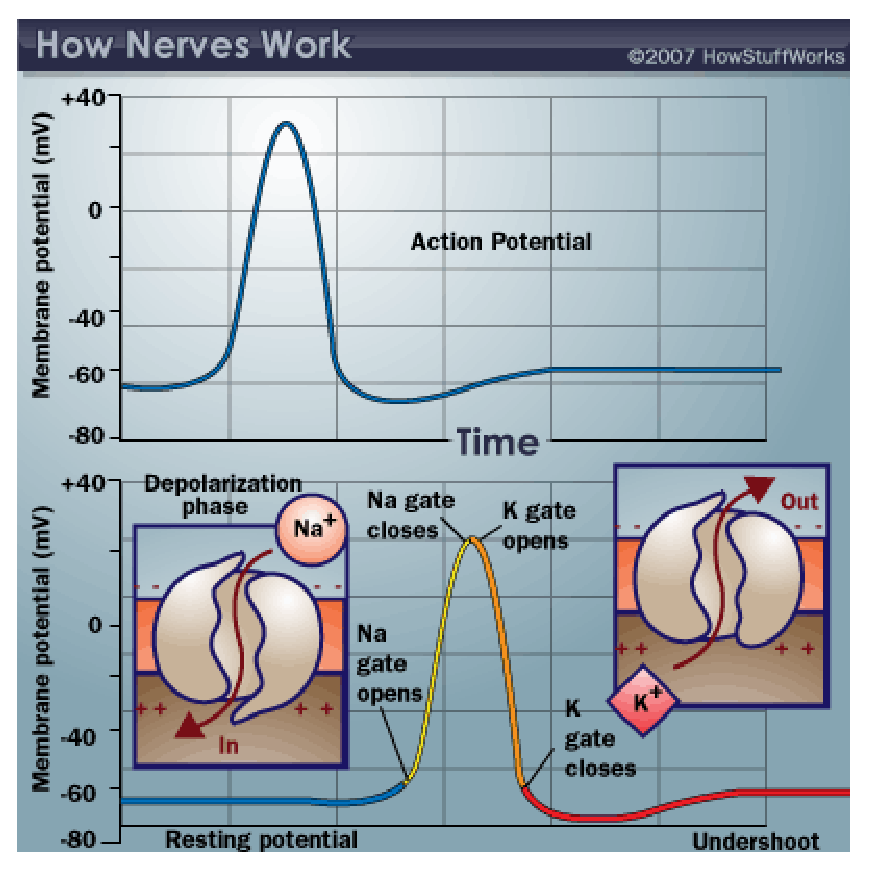
\includegraphics[height=5cm,
    angle=0]{./images/nodal-AP.eps}
    ,\includegraphics[height=5cm,
    angle=0]{./images/cardiac-AP.eps} }
  \caption{(A) Neuron AP; (B) Cardiac Purkinje AP}
  \label{fig:nerve-cardiac-AP}
\end{figure}

Depending on types of ionic channels, and their densities, APs are different in
shapes between species (Sect.\ref{sec:detail-ap-different}) and between
different cell types in a single species, Fig.~\ref{fig:nerve-cardiac-AP}.
In nerve cells, the duration of AP is about 1ms. In skeletal muscle cells, the
duration of AP is about 2-5ms. In cardiac myocytes, the duration of AP is in the
range 200-400 ms
\footnote{\url{http://www.cvphysiology.com/Arrhythmias/A010.htm}}.
The long AP in cardiac myocytes is characterized by a longer plateau, as shown
in Fig. \ref{fig:cardiac_AP} that is maintained mostly by $\Ca$ ionic currents.


Quantities related to AP include transient rate, the duration of the AP, the
plateau range, the replorarizing duration ...  Typically, a computational model
of cardiac cells need to replicate the AP of a specific species, with all of
such properties. Pathological conditions related to AP include the early after
depolarization (EAD) - Sect.\ref{sec:early-afterd-ead}, delayed after
depolarization (DAD) - Sect.\ref{sec:delay-afterd-dad}. We will learn the
quantitatively difference between AP in different cardiac cell types in
Part.\ref{part:compartmental_model}.

\begin{framed}
  In cardiac cells, T-type $\Ca$ channels is important in initiating AP (T =
  transient), while L-type $\Ca$ channels is important in sustaining an AP
  (L=long). Because of their rapid kinetics, T-type is often found in
  cells undergoing rhythmic electrical behavior (e.g. neuron cell bodies
  involved in walking/breathing, pacemaker cells (SA node and AV node)
  of the heart; while L-type channels are found in cardiac cells
  (i.e. ventricular myocytes).
\end{framed}

% in which L-type $\Ca$ channels is the major canals.
% , there are two general types of cardiac
% AP: pacemaker AP (or ``slow response'' AP) and non-pacemaker AP (or ``fast
% response'' AP), as shown in Fig.~\ref{fig:cardiac_AP}(B)(C). Non-pacemaker APs
% are found through the heart, except for pacemaker cells.  Here, we mainly
% concentrate on non-pacemaker APs


With different types of cardiac cells in the heart, there are two general types
of cardiac AP: non-pacemaker AP (or ``fast response'' AP) and pacemaker AP (or
``slow response'' AP), as shown in Fig.~\ref{fig:cardiac_AP}(B)(C).
\begin{enumerate}
\item Non-pacemaker APs (Sect.\ref{sec:fast-response-ap} are found through the
heart, except for nodal cells, with \ce{Ca^2+} influx prolonging the duration of AP to
  produce a characteristic plateau phase.

Examples of non-pacemaker cells are {\it myocardial cells} (atria and
ventricles), and {\it Purkinje fibre cells}.

\item Pacemaker APs (Sect.\ref{sec:slow-response-ap}) are found in nodal tissues
within the heart, and \ce{Ca^2+} influx involves in the initial depolarization
phase of  AP.
\end{enumerate}
\textcolor{red}{Here, we mainly concentrate on non-pacemaker APs}; though models
of pace-makers (e.d. nodal cells) are also described
(Chap.~\ref{chap:models-ap-nodal}). Examples of non-pacemaker cells are {\it
Atrial myocytes}, {\it ventricular myocytes}
(Chap.~\ref{chap:ap_ventricular_myocyte} and
Chap.~\ref{chap:ap_ventricular_myocyte_localcontrol}) and {\it Purkinje cells}
(Chap.~\ref{chap:models-ap-purkinje}). Fig.\ref{fig:ion_channel_roles_AP} shows
the roles of all types of ion channels at different phases of AP.
 

In muscle fibres, when the membrane is suddenly depolarized, the
potassium permeability of the membrane is increased; a phenomenon
known as {\bf K-activation} \citep{grundfest1961ime} or
{\bf delayed rectification}~\citep{hodgkin1949icu}.  After the AP is
maintained for a few seconds, the increase in K permeability
diminished and disappears completely, i.e. the stage of K-inactivation
occur. To hold the potential not to fall down so fast, it is the
influx of \ce{Ca^2+} that leads to the CICR process. This keep the
membrane potential for a long enough time, and cause a plateau shape
in the AP.

% in which L-type \ce{Ca^2+} channels is the major canals.


\begin{figure}[htb]
  \centerline{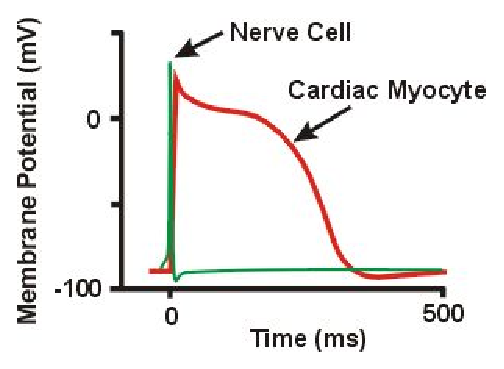
\includegraphics[height=4cm]{./images/action_potentials_compare.eps}}
    \centerline{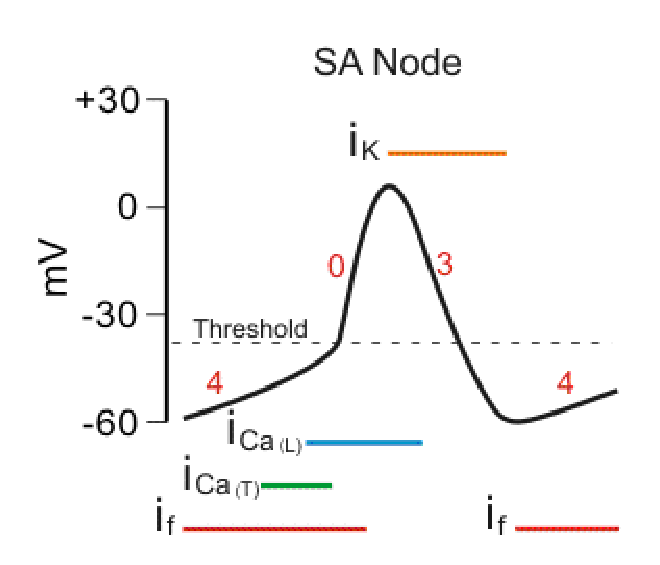
\includegraphics[height=5cm]{./images/pacemaker_AP.eps}, 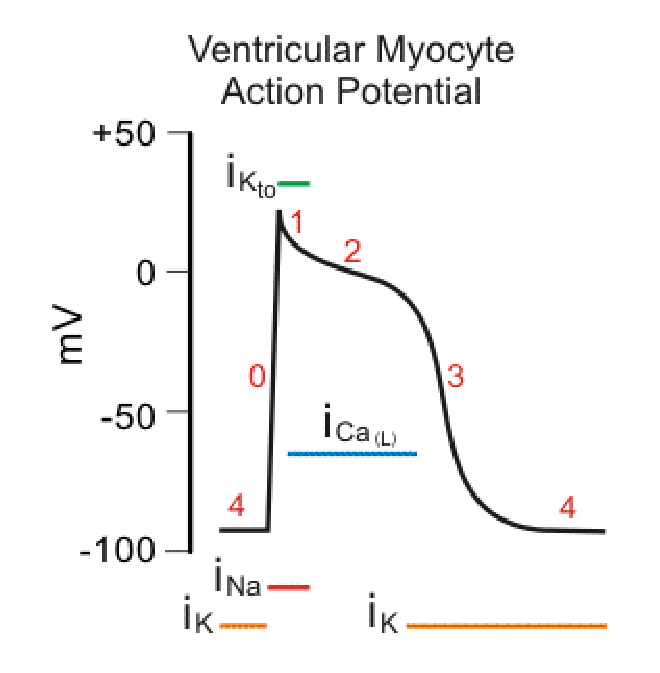
\includegraphics[height=5cm]{./images/ventricular_action_potential.eps}}
    \caption{(A) compare between nerve cell AP vs. cardiac
      non-pacemaker AP; Phases of a cardiac AP in (B) pacemaker cells,
      (C) non-pacemaker cells}\label{fig:cardiac_AP}
\end{figure}


\subsection{``fast response'' AP (non-pacemaker AP)}
\label{sec:fast-response-ap}

The ``fast response'' AP is caused by the relatively changes in fast
\ce{Na+}, slow $\Ca$ and \ce{K+} conductances and currents. Once
the AP is initialized, the cell become insensitive to stimulus. In
other words, the duration of time comprising phase 0, 1, 2, and part
of phase 3 is the time within that a new AP cannot be initiated. This
period of time is termed {\bf effective refractory period} (ERP) or
{\bf absolute refractory period} (ARP) of the cardiac cell. In other
words, during this time, the stimulation by an adjacent cell to the
examining cell does not produce new, propagated AP. Near the end of
the activation impulse, the cell may be re-activated, but with a
stimulus stronger than normal. This period is called
{\bf relative refractory period}.  In medicine, to prevent
{\it tachyarrythmias}, drugs are used to increase ERP to abolish
reentry currents.

\begin{figure}[hbt]
  \centerline{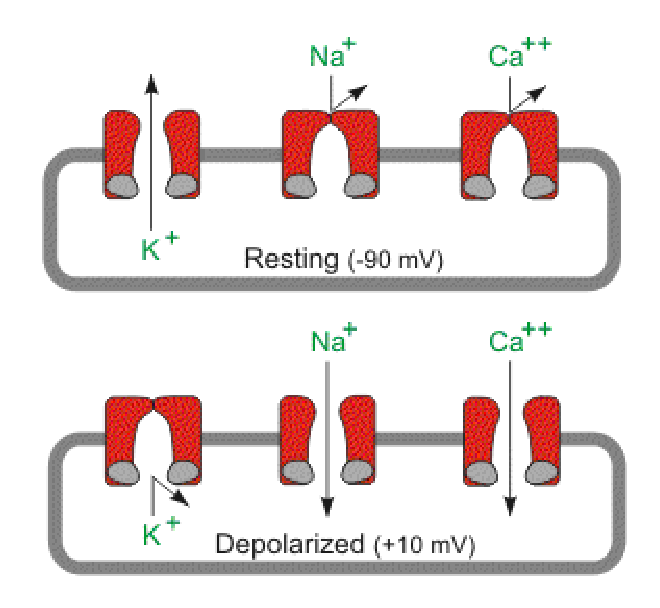
\includegraphics[height=5cm]{./images/channel_activation_AP.eps},
    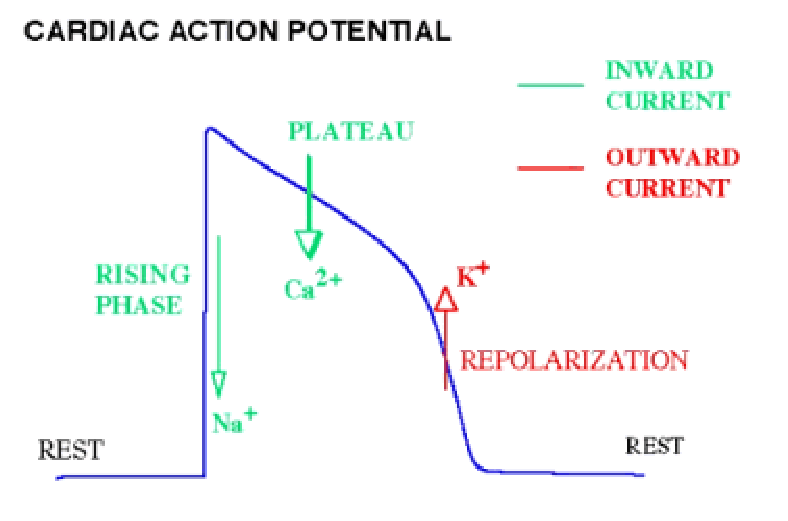
\includegraphics[height=5cm]{./images/cardiac-current.eps}}
  \caption{Activities of different types of channels during resting
    vs. action potential in non-pacemaker cells}
  \label{fig:channel-activity}
\end{figure}

Phases in a ``fast response'' AP, Fig.~\ref{fig:cardiac_AP}(C) or
Fig.~\ref{fig:channel-activity}:
\begin{itemize}
\item phase 4: the resting phase

  At resting phase, some \ce{K+}-channels are still active, especially
  I$_{\k1}$. In non-pacemaker cells, it has true resting potential (phase 4)
  as it remains near the equilibrium potential for \ce{K+} ($E_{\ce{K+}} \approx
  -90$mV). 

\item phase 0: the sharp rise - {\bf AP upstroke} - corresponds to the
  fast-inward of  \ce{Na+} current $I_\na$, and to a lesser extent of
  L-type $\Ca$ channels $I_\CaL$. 

  When the membrane depolarize to a threshold voltage, of about -70mV to -60mV,
  there is a rapid depolarization that is caused by a transient
  increase in intracellular [\ce{Na+}] through inward fast
  \ce{Na+}-channels, as shown in Fig.~\ref{fig:channel-activity}.
  This process changes the membrane potential away from $E_{\ce{K+}}$
  (negative) and move to $E_{\ce{Na+}}$ (positive). Na/Ca exchanger is suspected
  to play a role in abnormal trigger of AP in failing heart.

\item phase 1: first decay corresponds to the $\Na$-channel
  inactivation and the activation of the $V_m$-dependent transient
  outward $\K$ current $I_{to,1}$~\citep{sah2003}. A $V_m$-independent
  $\Ca$-dependent chloride current $I_{to,2}$ may also contribute, yet
  whether it's contributing to shape human AP is still
  controversy~\citep{ORourke1996}. $I_{to}$ is found in most species (canine,
  rabbit, human), but not in certain species (rat). 

  This {\bf notch} is apparent in ventricular myocytes (isolated from epi- and
  mid- myocardial regions, but not from endocardium) of some mammalian species
  (canine). During this time, the activation of L-type $\Ca$ channels also bring
  a small amount of $\Ca$ which brings $V_m$ to a more depolarized state. This
  is reflected by the shape of the AP dome. This amount of calcium is not enough
  to initiate actin-myosin cross-bridge; yet it can trigger a larger amount of
  $\Ca$ to be released from internal storage sarcoplasmic reticulum (SR/ER) via
  RyR2 gating channels.

\item phase 2: a plateau sustained by a balance between $I_\CaL$ and
  outward \ce{K+} channels (the rapid $I_\Kr$ and slow-activating
  delayed rectifier $I_\Ks$
  currents~\citep{horie1990,sanguinetti1990tcc} and the plateau $\K$
  current $I_\Kp$~\citep{yue1988ncp}), \ce{Na+}/$\Ca$-exchanger
  and \ce{Na+}/\ce{K+}-exchanger also play minor roles in this phase.

  During this phase, the membrane potential is held as a high voltage
  for a few hundreds of milliseconds, with low membrane conductance.

\begin{framed}
  Phase 2 is very important. Thanks to this voltage hold, the cardiac
  AP plays an important role in coordinating the contractility of the
  heart~\citep{kleber2004bmc}.
\end{framed}

\item phase 3: second decay (rapid repolarization) corresponds to the
  continue activating of $I_\Kr, I_\Ks$, and the inward rectifier $\K$
  current ($V_m$-repolarization-activated) $I_{K1}$.

  During this time, L-type channels are closed while \ce{K+} channels are still
  open. Further, the repolarizing induces more \ce{K+} channels to open, pulling
  the voltage back to the repolarized state, and even lower than the resting
  potential. Thus, to recover back to resting potential, the cell need to
  decrease the concentrations of $\Ca$ and $\Na$ using Na/K-ATPase pump,
  Na/Ca-exchanger, and SERCA-ATPase pump.
\end{itemize}


\begin{framed}
  
  The major difference between skeletal cells and cardiac cells is that:
  influx of \ce{Na+} quickly depolarize the skeletal myocyte and trigger
  calcium release from the SR. In cardiac myocytes, the release of
  $\Ca$ from the SR, however, is induced by $\Ca$ influx into
  the cell through a process called calcium-induced calcium-released
  (CICR) which is studied in the next chapter. So, the influx of $\Ca$
  is important in cardiac cells, but not in skeletal cells for an AP to
  initiate.
\end{framed}

At resting phase, the resting potential is maintained mainly by
the activity of some \ce{K+}-channels. In non-pacemaker cells, it
has true resting potential (phase 4) as it remains near the
equilibrium potential for \ce{K+} (about -90mV). 

When there is an electrical impulse, mainly due to the influx of
\ce{Ca^2+}, the membrane voltage is depolarized. This trigger the
opening of more low-voltage activated \ce{K+} channels.  At the
threshold voltage, of about -70mV, there is a rapid depolarization
that is caused by a transient increase in intracellular [\ce{Na+}]
through fast \ce{Na+}-channels, as shown in
Fig.~\ref{fig:channel-activity}.  This process change the membrane
potential away from $E_{\ce{K+}}$ (negative) and move to $E_{\ce{Na+}}$
(positive).

As shown in Fig.~\ref{fig:cardiac_AP}(C), the sharp rise (segment 0)
corresponds to the influx of \ce{Na+}. As the activity of \ce{K+}
channels is bi-stage. In other words, the high membrane voltage
deactivate the \ce{K+} channels. This causes a decay in membrane
voltage (segment 1). However, thanks to the release of \ce{Ca^2+} from
intracellular storage, via the CICR process, it held the membrane
potential as a high voltage for a few hundreds of milliseconds
(segment 2).  With a repolarizing efflux of \ce{K+} ions, the membrane
voltage then decreases rapidly (segment 3). The repolarizing doesn't
stop at the resting potential but go to a more negative value, then
slowly increasing to the resting potential before a next AP can
occur. This last stage is known as the {\bf afterhyperpolarization}
(AHP) stage\footnote{more information is covered in Appendix A of
  Computational Biology book}.
%  whereas the two decays
% (segments 1 and 3) corresponds to the sodium-channel inactivation and
% repolarizing efflux of potassium ions, respectively. There is also an
% extended plateau (2) in which the membrane potential is held as a high
% voltage for a few hundreds of milliseconds. This is the result from
% the activation of voltage-gated \ce{Ca^2+} channels. 
Thanks to this voltage hold, the cardiac AP plays an important role in
coordinating the contraction of the heart~\cite{kleber2004bmc}.

\begin{figure}[hbt]
 \centerline{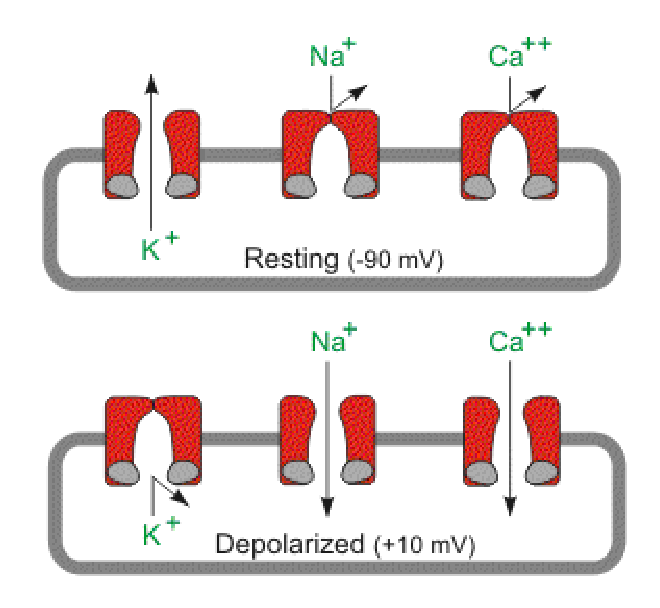
\includegraphics[height=6cm]{./images/channel_activation_AP.eps}}
 \caption{Activities of different types of channels during resting
   vs. action potential in non-pacemaker cells}
\label{fig:channel-activity}
\end{figure}

\begin{figure}[hbt]
  \centerline{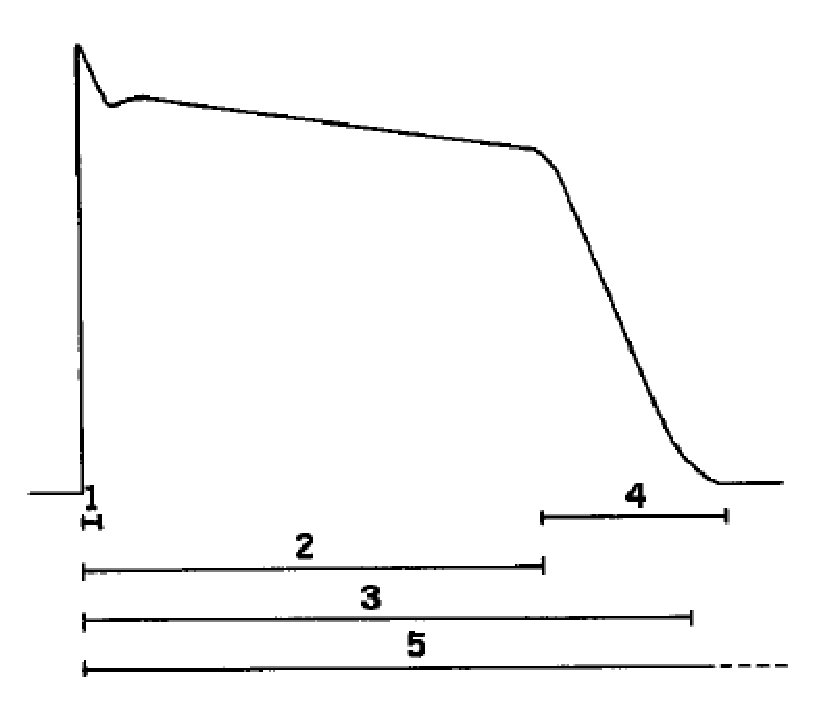
\includegraphics[height=5cm,
    angle=0]{./images/time_fast_AP.eps}}
  \caption{Time in fast AP: (1) depolarization, (2) absolute
    refractory, (3) total refractory, (4) repolarization, (5)
    automaticity cycle length (automaticity = the ability to initiate impulses)}
\label{fig:fast_AP}
\end{figure}

The ``fast response'' AP is caused by the relatively changes in fast
\ce{Na+}, slow \ce{Ca^2+} and \ce{K+} conductances and currents. Once
the AP is initialized, the duration of time comprising phase 0, 1, 2,
and part of phase 3 is the time within that a new AP cannot be
initiated, as shown in Fig.~\ref{fig:fast_AP}. This period of time is
termed {\bf effective refractory period} (ERP) or
{\bf absolute refractory period} (ARP) of the cardiac cell. In other
words, during this time, the stimulation by an adjacent cell to the
examining cell does not produce new, propagated AP.  In medicine, to
prevent tachyarrythmias, drugs are used to increase ERP to abolish
reentry currents.

In cardiac cells, T-type \ce{Ca^2+} channels is important in
initiating AP, while L-type is important in sustaining an AP. Because
of their rapid kinetics, T-type is often found in cells undergoing
rhythmic electrical behavior (e.g. neuron cell bodies involved in
walking/breathing, pacemaker cells (at SA node and AV node) of the
heart; while L-type channels are found in myocardial cells.

The major difference between skeletal cells and cardiac cells is that:
influx of \ce{Na+} quickly depolarize the skeletal myocyte and trigger
calcium release from the SR. In cardiac myocytes, the release of
\ce{Ca^2+} from the SR is induced by \ce{Ca^2+} influx into the cell
through a process called calcium-induced calcium-released (CICR) which
is studied in the next chapter.

\subsection{``slow response'' AP (AV node or SA node)}
\label{sec:slow-response-ap}

The ``slow'' response AP occurs in pacemaker cells found in the
sino-atrial (SA) node. We don't observe a transient in crease in phase
0 of the AP at the AV node as it is not dependent on fast \ce{Na+}
channels as in non-pacemaker cells, but instead generated by the
influx of the calcium through slow-inward L-type calcium channels.


The shape of the ``slow'' AP observed in Fig.~\ref{fig:cardiac_AP}(B)
is the result of the fact that all the ``fast'' \ce{Na+} channels are
blocked as soon as the membrane potential is depolarized to
a threshold between -40mV to -30mV. When this occurs, the AP can still be
elicited, however, the inward current is carried by only the inward \ce{Ca^+}
influx\footnote{\url{http://www.cvphysiology.com/Arrhythmias/A006.htm}}. As
a result, we get a slower AP.

As the membrane change from resting potential (about -60mV in SA node), to about
-50mV, T-type $\Ca$ channels open which brings $\Ca$ into the cells. The inward
$\Ca$ current further depolarize the cell. When the membrane potential reaches
about -40mV, another type of $\Ca$ channel (L-type) opens, which can bring the
membrane potential to the desired threshold (end of phase 4) to trigger the rise
of potential to the peak (phase 0). During phase 0, $\Na$ current and $\Ca$
current via T-type decreases. When membrane potential reaches the peak, the
outward $\K$ current becomes active, and L-type $\Ca$ channels become
inactivated and close, which decreases inward current and increase outward
current. This helps bringing membrane potential downward to the resting
value (near the reversal potential for $\K$ current, i.e. about -96mV) in SA
node.

So, the changes in membrane potential is brought about by changes in $\Ca$ and
$\K$ mainly, and to a lesser extent by $\Na$ movement across the membrane
through ion channels. The rate can be modified by external factors: autonomic
nerves, hormones, drugs, ions and ischemia/hypoxia. The non-pacemaker cells can
change into a pacemaker cells under certain conditions. E.g.: if a cell becomes
hypoxic (low oxygen supply).

\begin{framed}
  
  The primary pacemaker cells are those in sinoatrial node (SA node)
  with rate of about 70-100 beats per minute.  When cells in SA node are
  dysfunction, then cells from atrioventricular node (AV node) - area
  between the left atrial and right ventricle, within the atria septum -
  will take the role, with rate of about 40-60 beats per minutes. If
  cells from both SA node and AV node don't work, then cells (left and
  right branches) of the Bundle of His, as well as from Purkinje fibres
  are used, yet the rate is slower with 30-40 beats per minutes. 
\end{framed}
% 
% The shape of the ``slow'' AP observed in Fig.~\ref{fig:cardiac_AP}(B)
% is the result of the fact that all the ``fast'' \ce{Na+} channels are
% blocked as soon as the membrane potential is depolarized to
% -50mV. When this occurs, the AP can still be elicited, however, the
% inward current is carried by only the inward \ce{Ca^+}
% influx\footnote{\url{http://www.cvphysiology.com/Arrhythmias/A006.htm}}. As
% a result, we get a slower AP.

\subsection{AP in ventricular cells}
\label{sec:AP-ventricular-myocyte}

To do that, we need to know which ionic contribute to the AP, the
dynamics of individual types of channels. In the first half of this
book, we have discussed them already. In the second part of the book,
we will study in detail how they are combined to form a complex
system. This section will briefly review different ionic currents and
which one contributes to which phase.

The membrane potential of ventricular myocyte at rest is about -85mV. 

In human, at 1Hz pacing, AP amplitude was 100mV \citep{li1999}, 132mV
\citep{li1998}, and 135mV \citep{nabauer1996}. Phase 0 upstroke velocity
$(dV_m/dt)_\max$ (Volt/sec) measured experimentally in human ventricular
subepicardium and midmyocardium were 228$\pm$20 (V/s) \citep{drouin1995},
446$\pm 46$ (V/s) \citep{pereon2000}.

After a delay of 3-9ms from the beginning of the stimuls, free
$[\Ca]_i$ begins to elevate quickly as a result of SR $\Ca$ release,
and reaches its peak after an addition of
8-19ms~\citep{cleeman1991}. The elevation of $[\Ca]_i$ is quite
homogeneous~\citep{takamatsu1989}. 

\begin{framed}
  What to adjust?
  \begin{enumerate}
  \item increase or decrease the time constants of SR calcium release
    channel (e.g. from 2ms to 3.5ms) to adjust the delay to peak
  \item adjust the maximal rate constant of calcium release from JSR
    from, say 60 to 38 ms$^{-1}$, to obtain a peak calcium transient
    value of 1.0$\mu$M during a normal AP.
  \end{enumerate}
\end{framed}

% \subsection{Ionic currents}
% \label{sec:ionic-currents-3}

In cardiac ventricular cell membrane, there are mainly 6 ionic
currents\footnote{\url{http://www.cvrti.utah.edu/~quan/ep/paper.html}}: 
\begin{enumerate}
\item $I_{Na}$: a fast sodium current
\item $I_{si}$: a slow inward current (old term used in
  \citep{trautwein1973sic,beeler1977rap}; actually, is the calcium
  current)
\item $I_{K}$: a time-dependent potassium current
\item $I_{K1}$: a time-independent potassium current
\item $I_{Kp}$: a plateau potassium current
\item $I_b$: a time-independent background current
\end{enumerate}
\begin{eqnarray}
  \label{eq:396}
  I_{ion} = I_{Na} + I_{si} + I_{K} + I_{K1} + I_{Kp} + I_{b}
\end{eqnarray}
We have learnt some of them in the previous chapters, and we will
learn the others in detail in the coming chapters.

For a single ion channel, we can assume the ionic current is related
to the voltage by the Ohm's law
\begin{eqnarray}
  \label{eq:397}
  I(t) = g(t,V_m)\times (V_m-E_{rev})
\end{eqnarray}
The conductance is determined by the maximum conductance $\overline{g}$ and
the fraction of open channel. Based on Hodgkin-Huxley model, the
fraction of open channel is determined by the hypothetical activation
variable $m$ and inactivation $h$ raised to an integer power.
\begin{eqnarray}
  \label{eq:398}
  g(t,V) = \overline{g} \times m(t,V)^i \times h(t,V)^j
\end{eqnarray}
with $i,j$ are positive integer; $m,h$ are assumed to obey the
first-order kinetics given as
\begin{eqnarray}
  \label{eq:399}
  \frac{dx}{dt} = \frac{x-x_\infty}{\tau}
\end{eqnarray}
with $i,j,x_\infty,\tau$ are determined experimentally. % The sections
% in this chapter cover different models in chronological order.



\subsection{AP in different species}
\label{sec:detail-ap-different}

\subsubsection{Canine}
\label{sec:canine}

\subsubsection{Rat}
\label{sec:rat}


\subsubsection{Guinea pigs}
\label{sec:guinea-pigs}

% \subsection{Types of cardiac AP and its Phases}
% \label{sec:phases-cardiac-ap}


% Nevertheless, they can be described in explicit
% phases.  

% \begin{figure}[htb]
%   \centerline{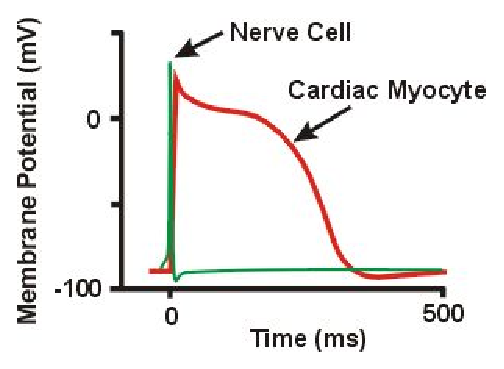
\includegraphics[height=4cm]{./images/action_potentials_compare.eps}}
%   \centerline{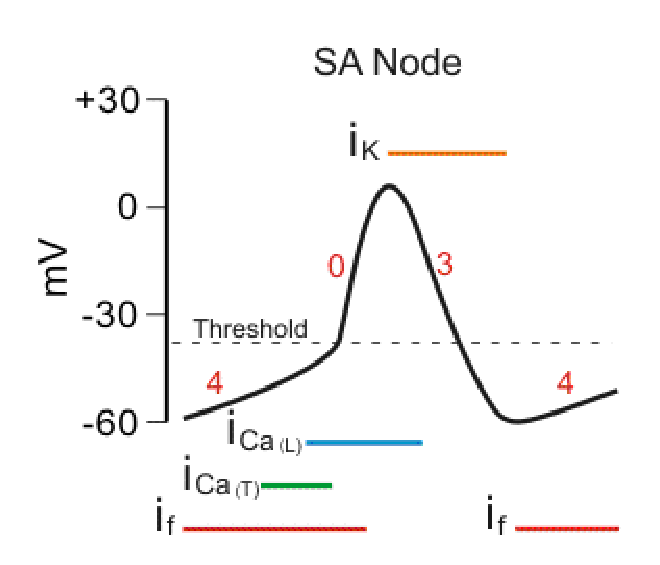
\includegraphics[height=5cm]{./images/pacemaker_AP.eps}, 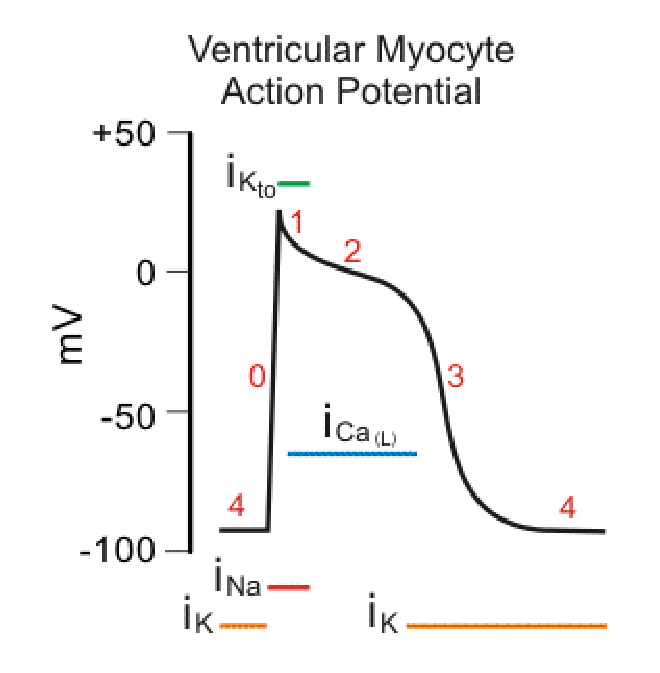
\includegraphics[height=5cm]{./images/ventricular_action_potential.eps}}
%   \caption{(A) compare between nervel cell AP vs. cardiac
%     non-pacemaker AP; Phases of a cardiac AP in (B) pacemaker cells,
%     (C) non-pacemaker cells}\label{fig:cardiac_AP}
% \end{figure}

% 
% \subsubsection{``slow response'' AP (pacemaker)}
% \label{sec:slow-response-ap}
% 
% 
% \subsubsection{``fast response'' AP (non-pacemaker)}
% \label{sec:fast-response-ap}


\subsection{Heart rate}

In contrast to skeletal muscle, cardiac muscle can contract on its own in the
absence of neural or hormonal stimulation. This property is called {\bf
automaticity}, or {\bf autorhythmicity}
\footnote{\url{http://www.as.miami.edu/chemistry/2086/NEW-Chap20/NEW-Chapter
20_part2.htm}}. The conducting system includes:
\begin{itemize}
  \item SA node (embeded in the posterior wall of the right atrium, near the
  entrance of the superior vena cava)
  \item AV node (at the junction between the atria and ventricles)
  \item conducting cells: 
\begin{enumerate}
  \item  conducting cells in the atria are found in {\it
  internodal pathways} (to distribute the electrical signal to atrial muscle
  cells as the impulse travels from the SA node to AV node). The connection between the AV node and
  AV bundle is called {\bf bundle of His} (the only electrical connection
  between the atria and the ventricles).
  \item conducting cells in the ventricles includes those in the AV bundle and
  the bundle branches, as well as {\it Purkinje fibers}, to distribute the
  stimulus to the ventricular myocardium. 
\end{enumerate}
\end{itemize}

Most of the cells in the conducting system are smaller than myocardial cells and
contains very few myofibrils. Electrical propgation before reaching the AV node,
it affects only the atria, as the fibrous skeleton isolates the atrium
myocardium from the ventricular myocardium. This takes about 50ms in human for
the stimulus to reach the AV node from SA node, then the atrium contraction
starts. The AV node cause a delay, i.e. the time to for the impulse to pass
through the AV node and enter AV bundle (about 100msec in human).
Then it follows a unidirectional propagation along the interventricular septum
within the AV bundle and enter the {\bf left/right bundle branches} (both
branches extend toward the apex of the heart, turn, and fan out deep to the
endocardial surface) before going into the {\bf Purkinje fibers}, and via the
moderator band, to the papillary muscles of the right ventricle. This phase
occurs very fast, about 25ms in human. The Purkinje fibers can conduct Ap very
fast (as fast as small myelinated axons). Finally, the impulse is distributed
throughout the ventricular myocardium; then the ventricular contraction begin,
starting from the apex of the heart (which also at about the time that the
atrial contraction completes). The entire process, from SA node to the complete
depolarization of the ventricular myocardium, in human takes about 225ms.

The papillary muscles begin contraction before the rest of the ventricular
myocytes as it receives the signal through the moderator band, rather than
through the Purkinje fibers. This contraction applies tension to the chordae
tendineae and brace the AV valves. This tension in the chordae tendineae
prevents the backflow of blood into the atria when the ventricle contracts. 

As the contraction in ventricular myocytes start from the apex of the heart,
under electrical-field simulation, we often see a wave that begins at the apex
and spread toward the base.

\begin{framed}
The delay in AV node is important  to give enough time for atrial contraction to
occur. Under testing condition, the AV node of a normal heart can conduct at a maximum rate of 230 AP
per minute (even if the SA node generates impulses at a faster rate). NOTE: When the
rate higher than about 180 beat per minute (bpm), the pumping efficiency start
to decrease. So, the rate 230 bpm can only occur when the conducting system is
damaged or stimulated by drugs.

The theoretical maximum limit of human ventricular myocytes pumping rate is
300-400bpm, depending on individual. 
\end{framed}


As different region of cardiac cells in the conducting system have their own
rate of spontaneous depolarization, it is the cells with the fastest rate that
determine the whole-heart rate. SA node has the fastest rate: 80-100 per
minutes. However, cells from the AV node has the lower rate: 40-60 AP per
minutes at normal condition. Certain cells in the Purkinje fibers has a slower
rate: 20-40 AP per minute. As SA node reaches the threshold first, it then
define the heart rate. Thus, SA node contains {\bf pacemaker cells} (natural
pacemaker). If this region is damaged, the heart still can beat, yet with a
lower heart-rate.




\subsection{Signal-Force relation}
\label{sec:sign-force-relat}

Essentially, the heart is a pump that squeezes to pump blood to other body
organs. Ultimately, the cellular signal in the heart is aimed to control the
excitation-contraction properly. This process is coordinated by a tightly
controlled mechanism via cell signalling in which $\Ca$ play a major role, a
{\it second messenger}. Starting from the nerve system, the rhythmic electrical
signal is transmitted to the sinoatrial (SA) node. The signal is then 
propagated to neighboring cells via gap junctions, into and through the right
and left atria,  initiating atria contractions, until they converge at the
atrioventricular (AV) node.

The signal, in the form of depolarization wave, from the AV node of the heart is
conducted through cells, the Hist bundle and the Purkinje fiber conducting
system to initiate the electrical depolarization and contraction of myocardial cells of
both ventricles. The membrane potential changes during a cycle of 
contraction-excitation is called action potential (AP), as depicted in 
Fig.~\ref{fig:cardiac_AP}. 

\begin{framed}
The rapid conduction in His-Purkinje network ensures almost uniform
and synchronous contraction of the ventricle. The slow conduction through AV
node determine and ensure the proper heart rate. The current flow through a
large number of ion channels and pumps underlies and coordinate these electrical
singals. The alteration of these critical balance of this multiple-current
pathway can lead to disruptive, often fatal, rhythm disturbances known as {\bf
cardiac arrhythmias}. Chapter \ref{chap:cardiac-diseases} will discuss in details. 
\end{framed}

In an AP, the global transient  increase of myoplasmic calcium leads to
a sequence of events in which contraction and excitation is the important one in
cardiac cells.

\begin{itemize}
\item contraction: The elevation of calcium $[\Ca]_i$ from 0.1 to $1\mu$M is the
result of the calcium release, either
from outside via SL or from internal calcium storage SR (Sect.\ref{sec:VICR_CICR}).
Part of the free $\Ca$ quickly bind to intracellular buffers, e.g. Calmodulin. 
The other part diffuse to the myoplasm and bind to Troponin (Tpn) to induce the
contraction. The mechanism of $\Ca$ release and the fraction of $\Ca$ released
from different sources is discussed in Sect.\ref{sec:local_control}. 

\item excitation: after the contraction, $\Ca$ need to be removed
  from the cytosol to allow cell relaxation.  The majority of $\Ca$ is
  sequestered back into the SR during each heart beat via
  {\bf SERCA pump} (sarcoplasmic/endoplasmic reticulum Ca-ATPase). For
  fast sequestration, some will be sequestered into mitochondria
  via $\Ca$ uniport and then being released out to be
  extruded across the sarcolemma via {\bf Na-Ca exchangers}, e.g. in
  rabbit and rat \citep{bassani1994rir}.
\end{itemize}

The fundamental unit of contraction in a cardiac muscle fiber is the {\bf
sarcomere} - the contractile apparatus between the {\bf Z-line} (or Z-disk).
However, there are recent evidences of the asymmetric between the left-right
of a sarcommere, suggesting that half-sarcommere is the true fundamental
unit~\citep{telley2006}. Modelling force-calcium signalling is described in
Chap.\ref{chap:force_calcium}.

% \section{Introduction}
% \label{sec:introduction-8}

\section{Ca2+-induced Ca2+-release (CICR)}
\label{sec:cicr}

The potential depolarization triggers the low-voltage-gated \ce{Na+}
channels, i.e. the fast \ce{Na+} current that facilitates the
transient increase in membrane potential to the peak. This happen in a
very short period of time compared to kinetics of other channels, so
in mathematical modeling, it's often modeled as an algebraic function
(rather than an ordinary differential equation).

The depolarized membrane potential, at a certain level, activate the
high-voltage-gated \ce{Ca^2+} channels, which yield a low-level influx of
\ce{Ca^2+} through $\Ca$ channels, mainly DHPR at T-tubules of the sarcolemma.
This is known as $I_{Ca,L}$ (Sect.~\ref{sec:L-type-Ca2+}). The \ce{Ca^2+} influx
trigger the opening of RyRs, which allow a larger calcium to be released from
the internal storage SR. This mechanism - calcium-induced calcium-release (CICR)
- is widely accepted since the discovery by Fabiato (1985) in skinned cardiac
cells, which subsequently observed in other cell types.

\begin{framed}  
  Calcium entries into the cardiac cell via the main gating L-type
  calcium channels (LCC or DHPR).  DHPR resides mainly in the
  transverse-tubules (T-tubules), though a lesser amount not in the
  subspace, which then given the name {\it non-junctional DHPR}.
  T-tubule is an inward invagination of the sarcolemma, filled with
  mucopolysaccharides, so that the potential depolarization can be considered
  homogeneous at every point of the cytoplasm. Mucopolysaccharides aka
  glycosaminoglycans are long chains of sugar molecules found throughout the
  body, often in fluid and mucus. 
\end{framed}

\subsection{Mechanism of $\Ca$ release: VICR vs. CICR}
\label{sec:VICR_CICR}

The electrical stimulus on the surface membrane leads to an AP causing the
depolarization along the surface and along the T-tubules.
In skeletal cells, the electrical depolarization can induce $\Ca$ release from
the underlying cisternae of the SR; thus $\Ca$ entry is not important for
initiating calcium release from SR. In cardiac cells, the depolarization trigger
the opening of $V_m$-gated L-type $\Ca$ channels (LCCs or aka dihydropyridine
receptor (DHPR)). The small influx of calcium via LCC then induces the larger
release of $\Ca$ from the terminal cisternae (and subsarcolemmal cisternae) of
the SR (and of the SL). So, the mechanism in skeletal muscle cells is VICR
(Voltage-induced $\Ca$ release) or depolarization-induced calcium release
(DICR), while that in cardiac cells is CICR ({\bf calcium-induced
calcium-release})~\citep{fabiato1975cic}.

\begin{framed}
  {\bf Historical facts}: 

  In 1972, Bassingthwaighte \& Reuter postulated that the influx of $\Ca$ from
  extracellular milieu {\it per se} is not high enough to trigger the
  contractile of the heart~\citep{bassingthwaighte1972cme}. Thus, they proposed
  that there must be some internal $\Ca$ storage; and the transarcolemmal $\Ca$
  influx doesn't trigger the myofilaments directly, yet through the induction of
  calcium release from this internal storage. Three years later, Fabiato-Fabiato
  has confirmed this hypothesis on skinned cardiac cells (cells with SR removed
  by microdissection)~\citep{fabiato1975cic} with the concept {\it
  calcium-induced calcium release}, and later on on other species (human, dog,
  cat, rabbit, rat, frog) ~\citep{fabiato1979cir}. Essentially, by their
  experiments, there is no influx of $\Ca$, of any magnitude could directly
  activated the myofilaments in skinned cardiac cells. Researchers also
  identified that the only internal storage for calcium is the sarcoplasmic
  reticulum (SR), not the mitochondria. Early literature reviews include
  ~\citep{ikemoto1977crs}, ~\citep{fabiato1983cir}.

\end{framed}

The strong buffering capacity in the cytosol, e.g. 100:1 \citep{bers1991ecc}
maintains a very low level of free calcium at rest, i.e. $10^{-7}$ M (or
$\approx 0.1\mu$M). The low resting $[\Ca]_{i,rest}$ compared to a much higher
concentration in the extracellular environment ($\approx 1.8$mM) facilitates a
large signal-to-background ratio $\Delta [\Ca]_i/[\Ca]_{rest}$ to be generated
just using a small amount of $\Ca$ added to the cytosol. The peak of average
free $[\Ca]_i$ during an AP is about 1$\muM$. Given the above buffering
capacity, it means the total cytosolic calcium to be released is about
100$\muM$ during systole. During relaxation, all this amount of released $\Ca$
need to be removed from the cytosol.

When $\Ca$ is globally released, a majority of free $\Ca$ then bind to the
$\Ca$-binding subunit of the thin filaments protein troponin to activate
contraction process. The cell senses the voltage signal by the change in calcium
concentration, causing it to contract or relax. 

Since 1990s, the accepted mechanism of $\Ca$-induced $\Ca$ release (CICR) is a
local control rather than global (cell-wide) process~\citep{Cannell2011}. The
detail is discussed in Sect.\ref{sec:local_control}. Under this local-control
theory, calciums are released at thousands of sites known as calcium release
sites (units - CRU) (Sect.\ref{sec:cru_calcium_release_unit}). Each CRU operates
independently at normal condition. In addition, the slow diffusion of $\Ca$ in
the cytosol is another factor to facilitate the local increase of calcium
easily, creating local response, without having to raise global calcium.
This is achieved thanks to many $\Ca$ buffers in the cytoplasm, e.g. parvalbumin
and vitamin D-dependent $\Ca$ binding proteins. This is energetically important,
as only a small energy is required to remove this local  transient.
 
\subsection{CICR - gradeness release: the importance of local control}
\label{sec:local_control}


% In the previous section, we also learned how $[\ce{Ca^2+}]_{i}$
% changes with ``on'' and ``off'' reactions in myocytes. 

\cite{fabiato1983cir} hypothesized that CICR occurs  through a process as
described as follows. The calcium influx increase the [free $\Ca$] in the
cytoplasm, which trigger the openings of  $\Ca$-mediated gates on the SR
membrane.
Now we know these gates are SR transmembrane ion channel - RyRs - with type2 is
the major isoform in ventricular myocytes. CICR a high gain (or amplification),
and re-generative process which is supposed to give all-or-none behavior.
However, experimental data shown that contractile amplitude is a smoothly {\it
graded} function of $V_m$~\citep{new1972}. It was then hypothesized that the
global elevation of free $[\Ca]_i$ is the summation of all local elevations at
different CRUs. This is the essential content of {\bf local-control theory}.

Cell signalling performs its function through frequency and amplitude of the
signal. For better control, another dimension is added, i.e. the spatial. Local
control guarantees only a small amount of calcium can perform its signalling
purpose. Also, it can target to a particular local region in the cell. However,
as pointed by A.V. Hill, signaling just by means of diffusion is not fast enough
to trigger a homogeneous and instantaneous change in calcium
signalling~\citep{hill1910pea, hill1949}. Given that electrical potential can
progate extremely fast (time constant is 100$\mum$, compared to calcium
diffusion about 1$\mum$. So, the cell must provides some means to use the
electrical potential to facilitate instantaneous change in calcium signalling. 

Using electron microscopy (EM), in cardiac cell, it shown that the T-tubule
(transverse-tubule) system, the deep invasion of the surface membrane found at
saromemre Z-lines that is found almost uniformly in the cardiac
cells~\citep{endo1964, porter1957}. So, T-tubules was suggested as a mechanism
to help bringing AP propagation quickly into the internal of the cell where it
can trigger $\Ca$ release from SR at almost simultaneously everywhere in the
cell. The microdomain at which $\Ca$ is released is called the dyadic subspace,
or calcium release site. The structure of a dyadic subspace is discussed in
detail in Sect.\ref{sec:cru_calcium_release_unit}. 

\subsection{CICR - high 'gain'}

The concept macroscopic or 'whole-cell' {\bf gain} in EC coupling has received
much investigation \citep{wier2007a}. During a voltage-lamp, high gain refers to
the fact that $\Ca$ to be released from SR is much more than $\Ca$ entering the
cell via L-type $\Ca$ channels (LCC). Interestingly, $I_\CaL$ at negative
potentials is much more efficacious in triggering SR $\Ca$ release than at
positive potentials.
Thus, gain is always higher at negative potentials. So, gain decrease with
voltage increase that approach calcium reversal potential.

Macroscopic $I_\CaL$ is the ensemble of single channel currents $i_\ca$ through
thusands of individual channels. Given $N$ as the total number of LCC in a cell,
and $P_o$ is the opening probability, then
\begin{equation}
I_\CaL = N.P_o.i_\ca
\end{equation}
with $P_o$ is a function of $V_m$. Then, the question is which of the 
two factors that control the EC gain: the single channel current $i_\ca$ or
the local $NP_o$ (i.e. at a sigle dyad). The impact of each of the two factors was studied
by \citep{altamirano2007}. Supprisingly, incease either $i_\ca$ or local $NP_o$
alone decrease EC gain, i.e. reducing either of them increase EC gain. Also, a
smaller $i_\ca$ at $V_\stim=+0$ mV may be a highly effective trigger of SR $\Ca$
release, and the redundancy of $\Ca$  channel openings at individual junctions
is critical to local control, i.e. reducing $NP_o$ has a stronger effect on EC
gain than does a decrease in $i_\ca$. So, most dyad need a single channel
opening and that can trigger $\Ca$ sparks, and more than one channel opening is
considerred redundant or wasted opening. The data then suggested that increasing
$i_\ca$ always decreases gain. So, at negative $V_\stim$, where there is less
channel opening during the stimulus, the gain is higher. 


Different ways are being used to define
{\bf 'gain'}:
\begin{enumerate}
  \item The peak SR $\Ca$ release flux divided by the peak flux of $\Ca$ across
  the cell membrane \citep{wier1994lce}. Here, 'gain' is unitless. At +10mV, the
  gain is about 12 in rat ventricle. However, as shown in
  \citep{shannon2000pfs}, peak $J_\CaL$ and peak $J_\text{SR,rel}$ SR calcium
  release are not at the same time.\footnotemark[1] 
    
  \item To study the effect of SR change, instead of using peak value, Shannon
  et al. used integration  \citep{shannon2000pfs}. Total calcium release divided
  by the total calcium current, i.e. $\int J_\text{SR,rel}/\int J_\CaL$.
  $\int J_\text{SR,rel}$ was obtained from total cytosolic calcium flux after
  all other fluxes into and out of cytosol were accounted for. Here, gain is
  about 10 at 'normal' SR calcium content of $\approx 0.1\mu$mol/L cytosol; and
  as high as 50 at extremely high $[\Ca]_\SRT$.
\end{enumerate}

\footnotetext[1]{Old papers used $F$, rather than $J$ to indicate flux. For
consistency throughout the book, we use $J$ notation.} 

\begin{framed}

\textcolor{red}{How to calculate flux}:   Here, the flux is defined as the net
rate of movement of $\Ca$ ions into or out of the SR per litre of accessible
cytoplasm. Unit: $J$ (Molar/sec or M/s). From the fluorescence data, free
$[\Ca]_i$ is calibrated using proper formula (Sect.\ref{sec:calibrate_Fluo}). 

\end{framed}

Net SR $\Ca$ flux was estimated about \ldots in guinea pig \citep{sipido1991}.
However, the actual SR $\Ca$ release flux ($J_\text{SR,rel}$) was \ldots in frog
skeletal muscle fibres \citep{rios1989}, and \ldots in intact cardiac cells
\citep{wier1994lce}. The formula being used is \citep{wier1994lce}.
\begin{equation}
J_\text{SR,rel} = \frac{d}{dt}[\Ca]_i - J_\text{SR,pump} - J_\text{SR,leak} -
J_{I_\ca} + \sum^N_{n=1} \frac{d}{dt}[\CaL]_n
\end{equation}
Here, the sign of $J$ is positive if the flux tends to increase $[\Ca]_i$, and
the units is chosen as mM/s. So, $J_\text{SR,pump}$ is negative in sign, while
$J_\text{SR,leak}, J_{I_\ca}$ are positive in sign,
Fig.\ref{fig:Wier1994_Fig1}(I).

The total $\Ca$ influx via LCC ($J_{I_\ca}$), which can be measured by
eliminating $\Na$ current, NCX, $\K$ currents \citep{balke1994}.
\citep{shannon2000pfs} blocked NCX by using 0 Na inside and outside the cell;
blocked mitochondrial influx by using mitochondrial uptake inhibitor RU360
inside the pipette. The transient of $\Ca$ is achieved by using voltage-clamp
(with 200ms pulse), with internal perfusion with $\Ca$ indicator.  The holding
potential was -40mV, and pulsed potential was ranging from -30mV to +80mVs (e.g.
-30, -20, 0, +20, +40, +60, +80mV). The peak $J_\text{SR,rel}$ achieved at a
clamp pulse potential of 0mV. Apparently, 'gain' of the system, defined as
$J_\text{SR,rel(max)}/J_{I_\ca(\max)}$ vary with membrane potential. As shown in
Fig.\ref{fig:Wier1994_Fig1}(II), the gain decline with more positive voltage
pulse (from -20mV to +20mV). At +10mV, the gain is about 12.


\begin{figure}[hbt]
  \centerline{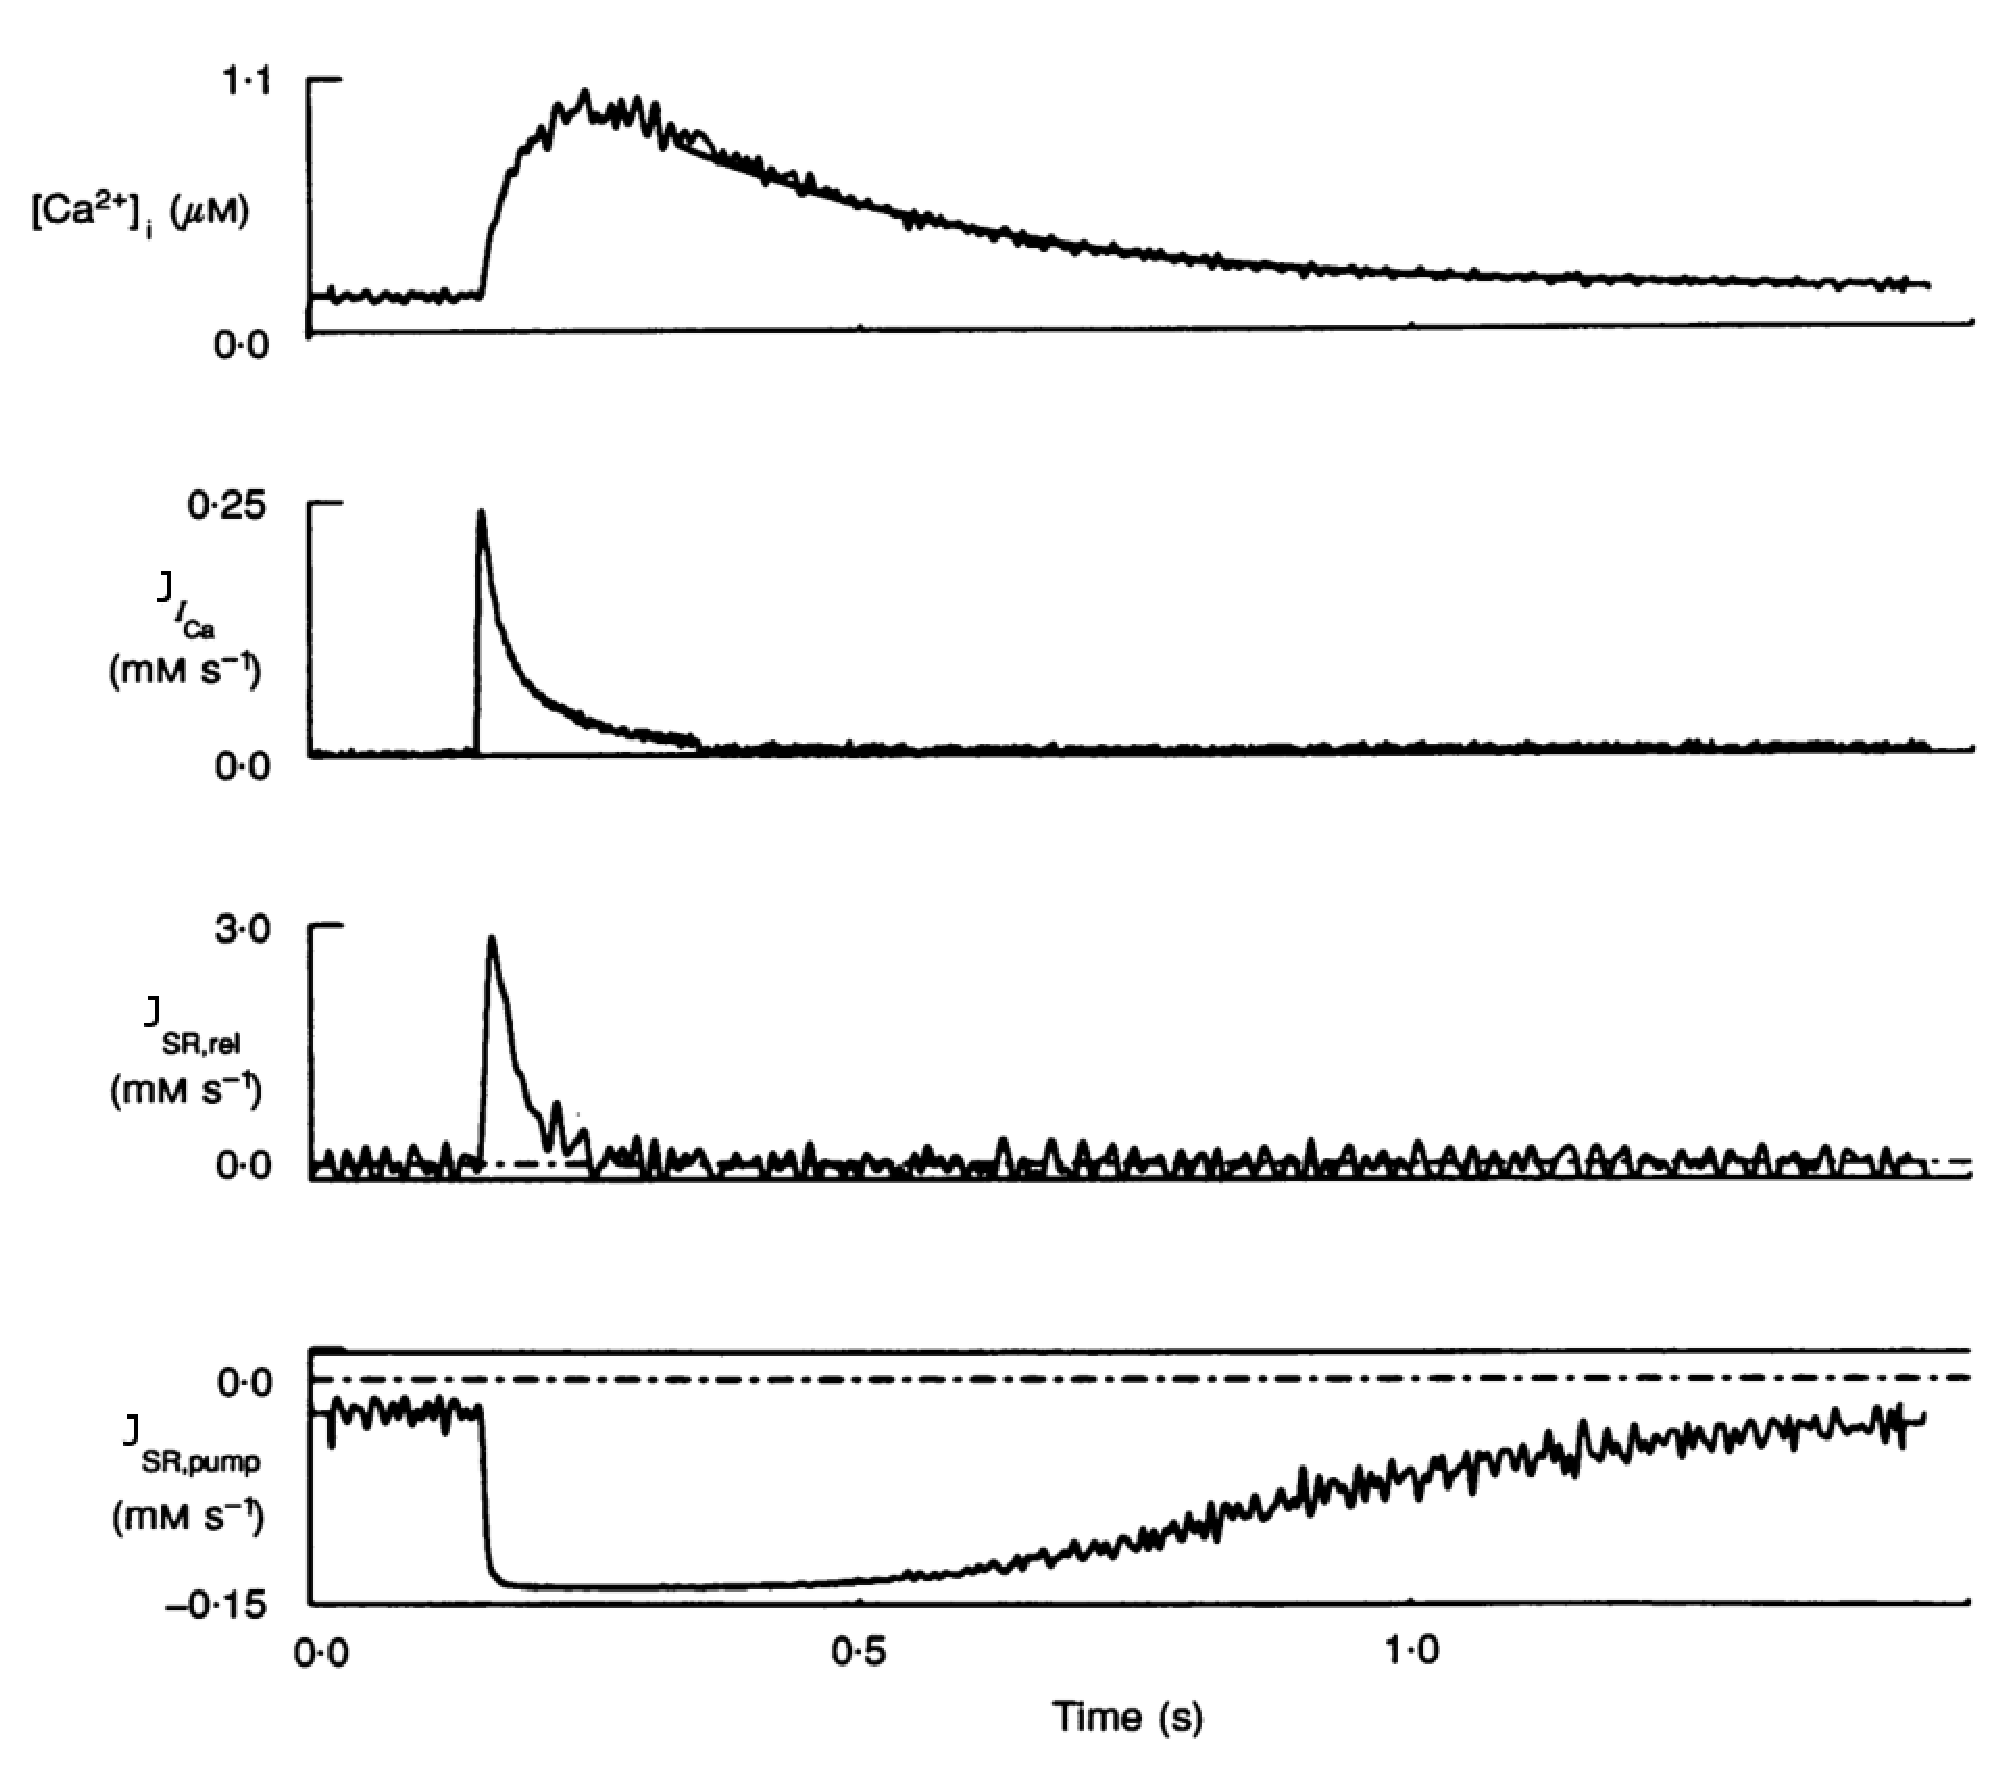
\includegraphics[height=7cm]{./images/Wier1994_Fig1.eps},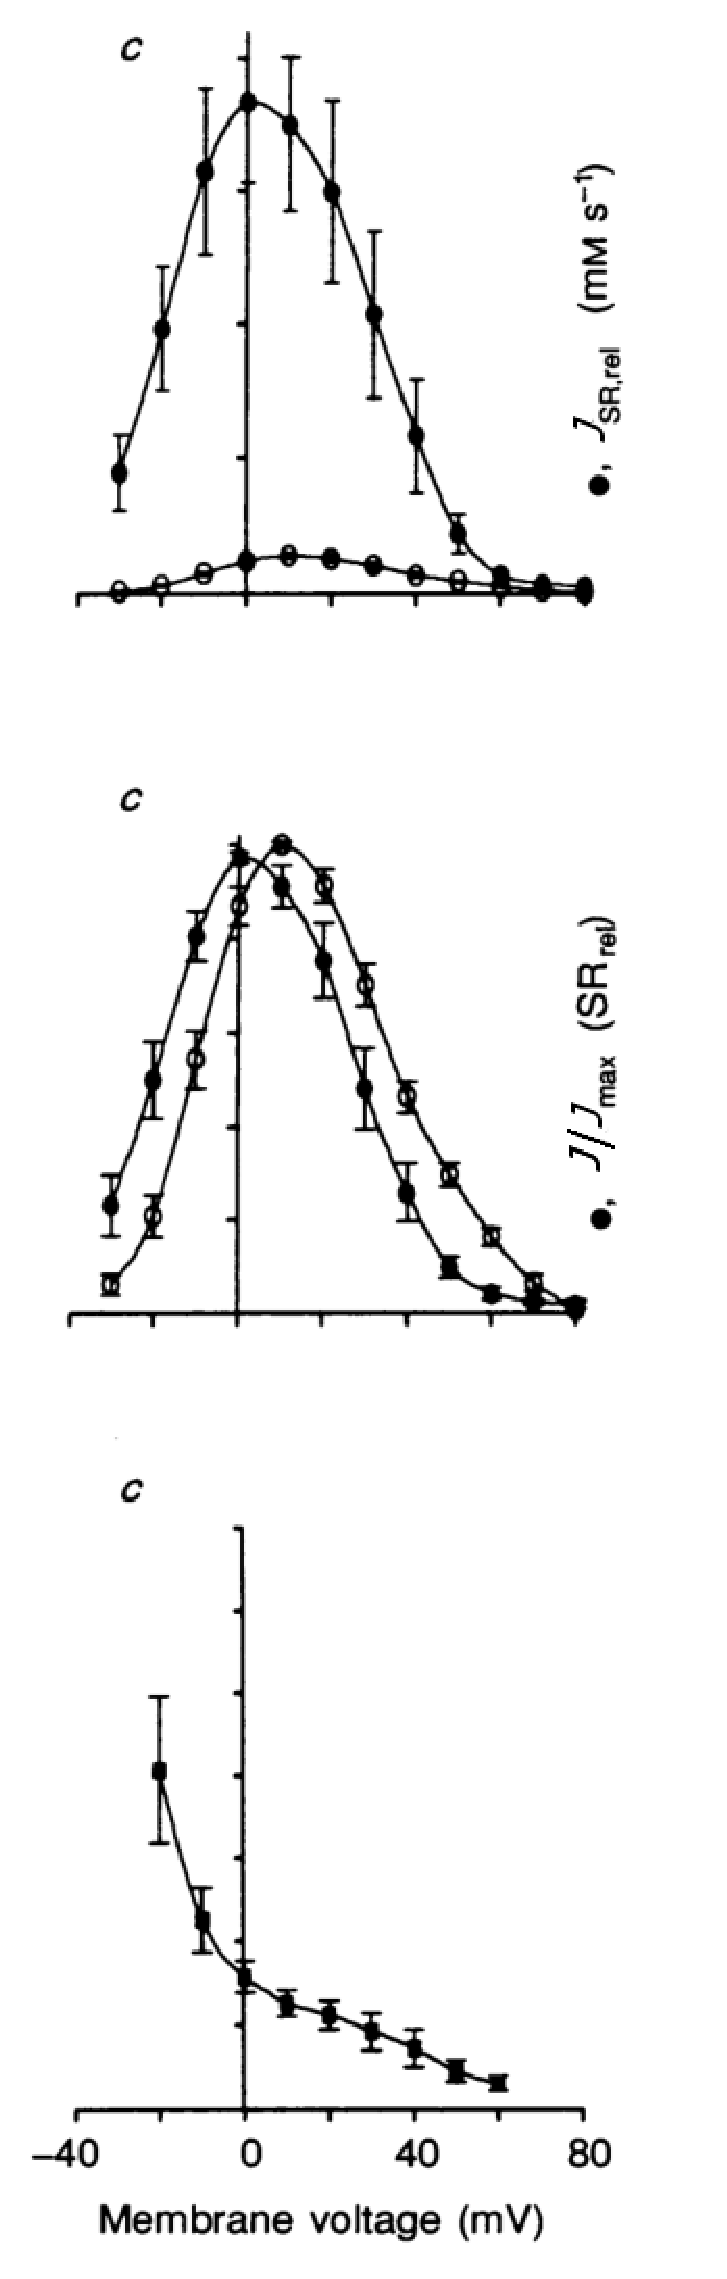
\includegraphics[height=7cm]{./images/Wier1994_Fig3.eps}}
  \caption{ (I) Simulation result in rat (from top to bottom): $[\Ca]_i$, flux
  through LCC, flux through SR, and flux through SR pump. (adapted from Fig.1
  \citep{wier1994lce}). The continuation line at the lowest figure indicate a
  constant leak into the cytoplasm $J_\text{SR,leak}$; (II) The average peak
  flux (mean$\pm$S.E.M for 9 cells): (A) $J_\text{SR,rel},J_{I_\ca}$, (B)
  normalized of (A); (C) the gain in rat ventricular myocyte is calculated using
  $J_\text{SR,rel}/J_{I_\ca}$}
  \label{fig:Wier1994_Fig1}
\end{figure}

In addition to voltage-dependency of gain, gain can be changed with pathology or
under different experimental conditions \citep{gomez1997,altamirano2007}. Gain
is expected to increase with a higher SR $\Ca$ load, giving the same $I_\ca$
current \citep{shannon2000pfs}. However, to answer the question whether the
relation is linear or nonline, \citep{shannon2000pfs} found out that during
anormal twitch, the fractional release is about 43\% of SR calcium, and about
4\% during low SR calcium load, and 60\% at maximal SR calcium load. So, they
hypothesized that fractional release was a steeply nonlinear function of
$[\Ca]_\SRT$ and $[\Ca]_\SR$. In other words, the fractional release is not the
simple function of $[\Ca]_\SRT$, but also the release process itself. 

SR calcium level was measured by using caffeine application
\citep{ginsburg1998}. The level of $[\Ca]_\SRT$ appears to reach a maximal level
of $\sim 100-120\mu$mol/L cytosol (given that cytosolic volume is about 14 times
larger than SR volume, so maximum SR level is about 14000-16800$\muM$).
As SR calcium content never depleted during the course, \citep{shannon2000pfs}
suggested a measurement to evaluate the maximum 'SR calcium depletion' during a
twitch
\begin{equation}
\text{SR calcium depletion} = \frac{\text{initial SR calcium} -
\text{ minimum SR calcium}}{\text{initial SR calcium}} \times 100
\end{equation}
So, given initial calcium is 96$\mu$mol/L cytosol, and minimum SR calcium
content is 53$\mu$mol/L cytosol; the SR calcium depletion is 45\%. Based on the
fact that no SR release was detected at SR loads below about 50\%, it's
suggested that this is the threshold for a 'shut-off' signals for SR calcium
release. Also, it's suggested that both extra SR calcium and intra SR calcium
(lumenal calcium) both affect to the gating of RyR2s.

\citep{cannell1994snu} estimated peak $J_\ryr$ can be 40x as high as
$J_{I_\ca}$; with the total $\Ca$ release flux summing over the course of AP is
about 10x higher than flux across $I_\ca$ \citep{isenberg1995, bers1991}. 

\subsection{Ion concentrations}
%\label{sec:ion-concentrations}

% TODO: define the 'resting stage' of cardiac cell, or excitable cell somewhere
% FIXME: something to fix

The physiological effect of ion concentration gradient across the plasma
membrane was studied since 1930s in erythrocytes by
Davson~\citep{davson1938spe,davson1940pec}. Many ions have a concentration
gradient across the membrane. For example, at resting stage of cardiac cells, it
has a higher \ce{K+} and lower \ce{Na+}, \ce{Cl-} intracellular concentration
than in extracellular fluid.

The role of $\Ca$ ions was ignored as $\Ca$ was wrongly believed to be
approximately equivalent between the two sides~\citep{overman1959pei}. Indeed,
when the cell is at rest, they are about 1000x difference in concentration, i.e.
$[\ce{Ca^2+}]_o\approx 1$mM, $[\ce{Ca^2+}]_{myo}\approx 0.1\mu$M).

Among these ions, the activity of $\Ca$ is of particular importance to the
normal contractile function of heart cell. ~\citep{glitsch1970} found that $\Ca$
influx is proportional to $([\Na])^2$ over a wide range of $[\Na]_i$. Among
different types of $\Ca$-channels, in ventricular myocytes, LCC is the dominant
(read Thermo-Stat book).  As calcium is a ubiquitous molecule in cardiac cells,
serving as a second messenger agent, in chap.\ref{chap:calc-handl-card}, we will
review different mechanisms to handle calcium signalling, focusing on {\it
ventricular myocardial cells}~\citep{rice2001mch}.






\subsection{global-control theory (common-pool model)}
\label{sec:glob-contr-theory}

Traditionally, CICR is hypothesized to follow the global control
theory or common-pool model. The essential feature of common-pool
model is that entering \ce{Ca^2+} and release \ce{Ca^2+} occupy a
common cytosolic space. It's the cytosolic \ce{Ca^2+} common pool that
control the RyR activity. The two main properties of CICR is high gain
and graded control. The ``graded'' \ce{Ca^2+} release from SR is
reproducible from the common-pool model. However, it doesn't have the
high gain property.

An apparent characteristic of calcium dynamics in cardiac cells is high-gain,
i.e. a small influx of calcium can trigger a much larger release of SR calcium.
There are different ways of definining 'gain', one of that is
$J_\text{SR,rel(max)}/J_{I_\ca(\max)}$ \citep{wier1994lce}. Although not all
common-pool models can be tested, Stern (1992) has proved rigorously that
common-pool models tend to give rise nearly ``all-or-none'' regenerative
\ce{Ca^2+} release, unless ``gain'' is relatively low~\citep{stern1992tec}.
Stern proved that a common-pool model with gain as high as 15 would be come
unstable for only a slightly increase in $[\ce{Ca^2+}]_{SR}$, e.g. 11\% change
(a phenomenon that is not observed until a very high calcium overload in cells).
Also, different gains were observed at different voltage clamp, a characteristic
would be impossible to achieve with common-pool models, with $\Ca$ currents of
the same amplitude \citep{wier1994lce}.

However, a small influx of \ce{Ca^2+} often trigger a much higher
release of calcium from SR, i.e. high ``gain''. In experiments, the
high gain can be from 10 to 100x. In addition, the release of calcium
is ``graded'', not ``all-or-none'' as postulated in the global control
theory. So, Bern proposed a ``local-control
theory''~\citep{stern1992tec}.

\subsection{local-control theory}
\label{sec:local-control-theory}

Local-control theory of calcium cycling was proposed first by
Stern~\citep{stern1992tec}. The macroscopically observed \ce{Ca^2+}
currents and cytosolic calcium transient is nothing more than the
summation of local events.  (NOTE: The $[\ce{Ca^2+}]_i$ notation
differs from that being used previously with $i$ means intracellular
that is equivalent to $[\ce{Ca^2+}]_{myo}$).

\begin{framed}
  LCC open very briefly (0.2 ms) and extremely infrequently
  ($P_o=0.004$ at the time of maximal macroscopic current). The
  current via a single LCC is constant during the brief opening. When
  the channel is open, the $[\ce{Ca^2+}]_i$ quickly raises to the
  level of several hundred mM, but falls extremely quickly (less than
  1ms) when the channel close~\citep{wier1994lce}. 
\end{framed}

In closed proximity to DHPRs are Ryanodine Receptors (RyRs). RyRs are
calcium gating of the network SR (NSR). The parts of the NSR that
branches closing to the DHPR is called the junctional SR (JSR) and
both from a local space called {\bf dyad} (dyadic subspace).  The
opening of a single LCC, at a specific dyadic subspace, will trigger a
small influx of \ce{Ca^2+} which subsequently trigger the opening of
RyRs to release \ce{Ca^2+} from the SR. Even though a single DHPR's
open can trigger \ce{Ca^2+} release, typically many DHPRs
simultaneously open during an AP, to create a safety margin to ensure
effective coupling. As a result, [\ce{Ca^2+}]$_{ds}$ will increase to
200-400$\mu$M.  The local [\ce{Ca^2+}]$_{ds}$ increase swiftly (within
$<1$ ms). 

\begin{framed}
  It's the local dyadic \ce{Ca^2+} signal, rather than by bulk
  cytosolic \ce{Ca^2+} levels, that control the CICR. The amplitude
  and profile of the macroscopic calcium elevation in the whole-cell
  is the summation (or recruitment) of these elementary \ce{Ca^2+}
  release events, known as \ce{Ca^2+} sparks.
\end{framed}

As a result, this local transient triggers the opening of
\ce{Ca^2+}-mediated RyR channels from the nearby junctional SR that in
turns allow more \ce{Ca^2+} from internal storage SR to be released,
as shown in Fig.~\ref{fig:schematic_CaRU}. All junctional SRs connect
to a common pool of calcium storage, i.e. the {\bf network SR}.

The more calcium in the subspace, the more RyR channels open, which
eventually lead to more calcium release. So, from a small calcium
influx, it can leads to a larger amount of calcium release from the
SR. This mechanism is thus called calcium-induced calcium release.
This was first discovered by Fabiato in 1975~\citep{fabiato1975cic}.

\begin{framed}
  \textcolor{blue}{Utilizing intracellular \ce{Ca^2+} rather than
    relying solely on \ce{Ca^2+} entry to trigger muscle contraction
    limits the danger of exposing the intracellular compartments to the
    essentially infinite extracellular \ce{Ca^2+} pool that would be
    toxic}.
  In almost cases, the release of intracellular \ce{Ca^2+} involves the
  activation of either ryanodine receptors (RyRs) or
  inositol-1,4,5-trisphosphate (IP3) receptors (IP3Rs). Thus, RyR ans
  IP3R are \ce{Ca^2+}-mediated channels.
\end{framed}

The observation of local $[\ce{Ca^2+}]_i$ transient was not feasible
until 1993, when Cheng et. al use confocal microscopy with
fluorescence calcium indicator on quiescent rate cardiac
cells~\citep{Cheng1993Calciumspark}. This local elevation of calcium
is coined \ce{Ca^2+} spark.


\section{Spatially-dependent encoding scheme}

Calcium signalling is regulated at both temporal (frequency) but also spatial
aspect (the increase is locally or globally). The release or elevation of
calcium are hold at microdomain scale scattering every where in the cell. This
can direct $\Ca$ signal in a very precise way to a very specific subcellular
targets. The spatial restriction in calcium elevation is guaranteed by virtue of
strong buffering and slow diffusion. This has lead to the concept of local
control and its importance in regulating calcium signalling.

Typically, a signal is encoded via amplitude and frequency-dependent coding
schemes. So, the adding of spatially-dependent coding scheme in calcium
signalling allows the use of very simple ions, in versatile purposes.
The microdomain where $\Ca$ are released is known as calcium-release site, or
calcium-release unit (CRU). 

%  and
% Chap.\ref{chap:ap_ventricular_myocyte_localcontrol} discuss whole-cell model
% using local control mechanism.

\begin{framed}
  The spatially-dependent encoding scheme is also found in other
  signalling pathways that depend on diffusible messengers,
  e.g. cAMP~\citep{fischmeister2006} or nitric oxide
  (NO)~\citep{garthwaite2005}.  Here, cAMP is localized by
  phosphodiesterases (Sect.\ref{sec:PDE}) shielding the site where cAMP is
  produced.  NO is unstable and shortlived; thus can only act over a very short
  distance.
\end{framed}

In the early days of 1990s, the resolution of microscopy is not high enough to
detect the structure of these microdomain. Nevertheless, the idea of local
control was first suggested by \citep{lederer1990, niggli1990} with the term
{\bf fuzzy space} for NCX ~\citep{lederer1990}. Despite the apparent differences
in the mechanism of EC coupling, it's believed that there's a dyadic junctions
in cardiac cells (Sect.\ref{sec:dyad}) that are equivalent to skeletal muscle
triads (Sect.\ref{sec:triad}).

Both triad and dyad can be called {\bf couplons}. In skeletal muscle, triad
doesn't have DHPR; yet the lipidbilayer with a cluster of RyR also forms a
stochastic functional unit (SFU) called {\bf couplons} ~\citep{stern1997}. In
cardiac, {\bf couplon} refers to a similar structure with a cluster RyR2 on jSR
and a few L-type $\Ca$ channels (LCC) on the T-tubule\citep{carl1995,
franzini_armstrong1999ssd}. Due to the majority of $\Ca$ are released from here,
its other name was calcium release units (CRU or CaRU). The spatial setting of
the two types of channels is called the functional release unit (FRU).

\subsection{CRU - Microdomain $\Ca$ signalling}
\label{sec:cru_calcium_release_unit}




% The volume of the restricted space is given \begin{equation} \label{eq:243}
% V_{ds} = (\text{junctional gap}) \times (\text{area of functional unit})
% \times (\text{number of functional unit}) \end{equation} Experimental result
% gave the value $V_{ds} = 1.485 \times 10^{-9}\mu l$, which is about 4 orders
% of magnitude smaller than that of the myoplasma $25.84 \times 10^{-6} \mu l$.
% Here, the ``local control'' treats L-type $\Ca$-channels and juxtaposed $\Ca$
% release sites as stochastic CaRU.

In general, there are three subtypes of CRUs in cardiac muscle that differ in
geometry, but the same molecular components, as shown in
Fig.\ref{fig:couplons_3types} \citep{franzini_armstrong2005}. Each cell type may
have one or all of these CRUs. The first one is the one we have discussed so
far, i.e. a couplons between LCCs on the T-tubules (and possibly axial tubules)
and RyR2s forming a dyadic subspace \citep{asghari2009}. The second one is
peripheral coupling, formed by RyR2s and the surface membrane (plasmalemma).
The third one, found in Purkinje fibre, known as {\bf corbular SR}, a JSR
domain located within the cells with RyR2s yet does not associate with either
plasmalemma or T-tubules. RyRs in the third one face calcium in the myoplasm and
aka rogue RyRs.

\begin{framed}
Corbular JSR is the mammalian homologue of the extended JSR first described in
birds \citep{jewett1971}. Corbular JSR has been described in rabbit atrial cell
\citep{jorgensen1993}. 
\end{framed}

\begin{figure}[hbt]
  \centerline{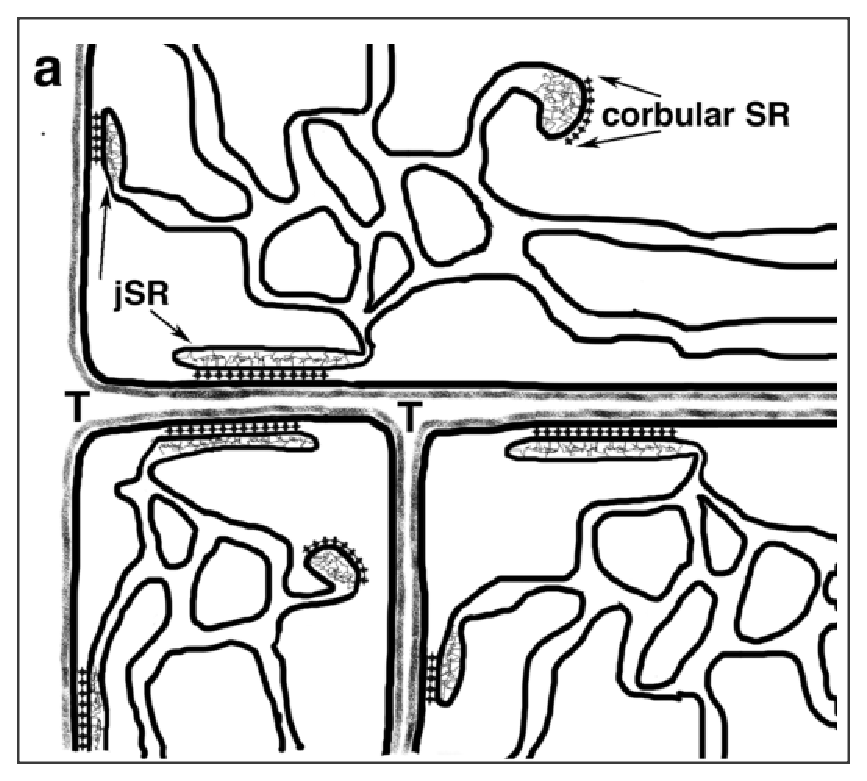
\includegraphics[height=5cm,
    angle=0]{./images/couplons_3types.eps}}
\caption{3 types of couplons \citep{franzini_armstrong2005}}
\label{fig:couplons_3types}
\end{figure}

During embryonic stages of cell developments, the second types appears first.
Then, T-tubules system is formed and thus creating dyads and corbular SR. For
the first two types (peripheral couplings and dyads), even both contains LCCs
and RyR2s, the DHPR:RYR ratio can be different. The second one is
believed to contribute a significant role in E-C coupling during the early stage
of cell development. The third one is believed to support spark-induced
spark propagation.

Due to the high resolution, it's very hard to know how RyRs are organized. In
terms of modelling, the early models assumed they activated and inactivated
altogether. So they modeled calcium release as a point source. Later on, a more
realistic approach that consider the allosteric interaction between neighboring
RyRs via domain 6 of the RyR2 molecule. More detail of computational models will be given in
Chap.\ref{chap:sparkology-study-ca}. 

Not until recently, we have some initial clues how RyR2s are organized in a
cluster. \citep{asghari2012} claimed that there are couplons that lie outside
RyR2-LCC dyad. A statistical analysis showed about 10-15\% of dyads also
associated with NCX \citep{scriven2000}. However, the role of NCX is still
controversal. A common hypothesis is that NCX can move $\Ca$ into the cell, and
thus triggering $\Ca$ release from  SR, forming ``eager'' $\Ca$ spark sites
\citep{Larbig2010}. NCX is also hypothesized to keep dyadic calcium level low to
minimize $\Ca$-dependent inactivation of LCCs, to maximize the availability of
LCCs for the next systole \citep{sher2008}. A smaller portion (3-5\%) of
couplons, the RyR2 cluster is in closed proximity to caveolin-3 rather than
LCCs.


\subsection{Size of a CRU: LCC/RyR2s ratio}
\label{sec:CRU_size}


\citep{wibo1991} reported that in rat ventricular myocytes, the density of LCC
and RyR2 were 84/$\mum^2$, and 765$/\mum^2$, respectively. In the body muscle of
arthropods, the density of RyR to be 1275-1890/$\mum^2$ translates to 15-28
RyR2s residing on a square patch of jSR membrane area of
$L_\text{cleft}=0.1-0.15 \mum$. The architecture of CRUs in the cardiac muscles
of vertebrates and arthropods are found to be similar \citep{takekura2002}.

Using electron micrographs, other studies suggested that at each dyadic
subspace, depending on species, RyR2s form the cluster of size 10-300 channels
in a 2 dimensional crystal-lattice array on the surface of SR release
\citep{franzini_armstrong1997,franzini_armstrong1998,franzini_armstrong1999ssd}.
This, along with the apposed L-type $\Ca$ channels, form the so called CRU.
~\citep{franzini_armstrong1999ssd}, using electron micrographs,
  show RyR clusters as densely localized in the Z-disk (or Z-line as
  view in 2D image) vary from 30-270 RyRs (depending on species) with
  high skewness to the left. Individual RyRs are visible as ``feet''
  in the image. A group of RyRs immediately adjacent to each other (or
  DHPRs, or other junctional SR proteins) form a functional group,
  known as ``couplons''~\citep{stern1997,rios1997}. A triad contains 2
  couplons, one on either side of the T-tubule, and act independently
  of each other. A dyad, and peripheral coupling, is a couplon
  each~\citep{sommer1998}.
 
 \begin{framed}
    
    Two geometrical factors that are constants in all types of CRUs: (1)
    the size of the junctional gap separating SR and T-tubule (10-12nm),
    and (2) the tight, ordered clustering of ``feet''.
    \begin{itemize}
    \item In skeletal muscle, feet are arranged in tetragonal
      disposition with center-to-center distance of 29nm.
    \item In cardiac muscle, feet are disposed at regular intervals
      approximately equal to those in skeletal muscle, with unknown
      parameter of the disposition.
    \end{itemize}
    The number of feet per couplons varies from skeletal cells and cardiac
    cells are shownn in Table~\ref{tab:Feet_couplon_skeletal} and
    Table~\ref{tab:Feet_couplon_cardiac},
    respectively ~\citep{franzini_armstrong1999ssd}.
  \end{framed}

 \begin{table}[hbt]
    \begin{center}
      \caption{Size of couplons (CRU size) in skeletal muscle}
      \begin{tabular}{ccc} 
        \hline
        Source & Muscle type & Average \# feet per couplon \\ 
        \hline\hline
        rat & fast twitch (EDL) & 38 (16-71) \\
        rat & slow twitch (soleus) & 24 (9-45) \\
        guinea pig & fast twitch (wh. vastus. lat.) & 34 (9-64) \\
        guinea pig & med. twitch (red vastus lat.) & 24 (9-45) \\
        guinea pig & slow twitch & 17 (7-27) 
      \end{tabular}
    \end{center}
    \label{tab:Feet_couplon_skeletal}
  \end{table}

Typically, RyR2 are assumed to form a dense matrix. From recent experimental
data, the dyad are not fully filled by RyRs. However, each is a ``supercluster''
containing many smaller RyR groups (archipelagos)
\citep{Baddeley2009,hayashi2009}. The number of RyR groups activated at a
release site is unknown. However, as the distance between archipelagos is small
(about 3 RyR monomer wide, or $<$ 100 nm edge-to-edge), one would still expect
all of them to expose to high $\Ca$ and all activate. The width of an RyR
monomer is about 30 nm.

  \begin{table}[hbt]
    \begin{center}
      \caption{Size of couplons (CRU size) in cardiac muscle}
      \begin{tabular}{ccc} 
        \hline
        Source & CRU type & Average number of feet per couplon \\ 
        \hline\hline
        rat left ventricle & dyads & 267 \\
        mouse left ventricle & dyads & 128 \\
        & peripheral coupling & 150 \\
        canine left ventricle & dyads & 90 \\
        & peripheral coupling & 61 \\
      \end{tabular}
    \end{center}
    \label{tab:Feet_couplon_cardiac}
  \end{table}

\citep{soeller2007} used immunocytochemistry combined with 3D imaging

The number of DHPR varies from 10-100\% of the number of RyRs~\citep{Sun1995}.
\citep{mejia-alvarez1999} estimated the ratio DHPR:RyRs is about 10:75 (assuming
$i_\ryr=0.05$ pA if all are open during activation, compared to 0.5pA measured
under physiological condition). Depending on species, \textcolor{red}{the ratio
RyR:DHPR can vary} from 10:1 to 4:1, e.g. about 4:1 to 6:1 \citep{wang2001},
about 5.6 in guinea pig, 5.6:1 in human \citep{bers1992}, and 7.3:1 in
rat~\citep{bers1993rrd}.
Recent data showed that each CRU has 5-20 L-type $\Ca$ channels (LCC) on the
T-tubule, and 50-300 RyRs on the junctional-SR (JSR) in closed proximity to the
LCC~\citep{chen-izu2006tdd, bers2008cca}. The total number of RyRs is about
$10^6$ RyR2 per myocyte.


However, in cardiac cells, DHPR are randomly positioned relative to
RyR lattice. This is in contrast to regular arrangement of DHPR in
skeletal muscle. For simplicity, some studies assumes that the gating
of a cluster of RyRs channels is either fully open or fully closed in
an all-or-none manner~\citep{williams2007pda}. Thus, the exact number of
RyR channels is unimportant and can be considered as a single
megachannel. However, the stochastic simulation of ion channels gating
in the CRU is required for an adequate understanding of calcium
dynamics.

Sparks originate from a cluster of 10-40 RyRs\citep{inoue2003}. 
Chap.\ref{chap:sparkology-study-ca} will discuss in
detail different computational models for $\Ca$ spark.

In a CRU:
\begin{itemize}
\item The number of RyRs in a subspace varies from species to species, with
  an average of about $\sim$ 100. When RyRs incorporated into planar
  lipid bilayers can exhibit coupled gating, i.e. two or more channels
  exhibit synchronized openings and closings. 

\item The number of DHPR is smaller than that, with the ratio RyR:LCC
  ranges from 4:1 to 8:1, depending on species.
\end{itemize}


\subsection{Dyadic volume}

The restricted volume between the T-tubule and the SR is called the cleft space.
The junctional distance between the T-tubular membrane and SR membrane is about
10-15 nm apart \citep{langer1996, franzini_armstrong1999ssd}, and
100-400 nm in diameter. This allows the sufficient voltage change triggering the
$\Ca$ release from SR via RyR channels, as well as imposing spatial limitation
of the signal \citep{franzini_armstrong1997}. 

Given the above dimension, the volume of the cleft, i.e. dyadic subspace volume
$V_\ds$, is estimated about 1.0-20.0$\times 10^{-13} \muL$ (if a cylindrical
cleft is assumed).


\subsection{Number of CRUs and its 3D distribution}
\label{sec:3d-distr-carus}

% The number of CRUs can be estimated as \begin{equation} \label{eq:869} N =
% \frac{V_\text{cell}}{l_L.l_T^2} \end{equation} ~\citep{satoh1996svr} estimated
% the average cell volume $V_\text{cell}=30$pl, which yields $N\approx 20,000$
% CRUs.
The number of CRUs was estimated about 20,000. The number of peripheral RyRs
clusters is about 10,000 with 30 RyRs per cluster. They are called extra-dyadic
RyR \citep{asghari2012}. These RyRs are suggested to locate near caveolin-3
(Cav3).


\begin{framed}
  In a ventricular myocyte, there is a large number of CRUs spatially
  distributed throughout a cell. A ventricular myocyte has between
  10,000 to 100,000 CRUs.  The side of the CRU is about 50nm in height
  and 10nm in width and 50nm in deep.  The $\Ca$ sparks are
  highly localized ($\sim 1\mu$m) and time ($\sim$ 20 ms).
\end{framed}

\begin{itemize}
  \item \citep{carl1995} used double labeling immunofluorescence and laser
  scanning microscopy showed transversely oriented bands of about 2$\mum$
  intervals along the whole length of the cell.
  
\item ~\citep{parker1996csi}, using ``home-made'' confocal microscope,
  reports an average transverse separation of 0.76$\mu$m and average
  longitudinal separation of 1.8$\mu$m. The space along the trasverse direction
  is smaller, and also less regular than in longitudinal scans. 

\item \citep{soeller1999} estimated mean transverse spacing is about 1.8$\mum$.
   
\item ~\citep{chen-izu2006tdd}, using immunolabelling and confocal
  microscopy\footnote{BioRad Radiance 2000} (with resolution
  0.25$\mu$m), reports an average transverse separation of
  $l_T=1.05\mu$m in ventricular myocytes (and 0.97$\mu$m in atrial
  myocytes) and average longitudinal separation of $l_L=1.87\mu$m in
  ventricular myocytes (and 1.69$\mu$m in atrial myocytes). The size
  of a cluster is 250nm, suggesting about 100 RyRs in a cluster. In
  addition, they found peripheral RyR clusters between the Z-line
  (known as {\bf intercalated RyR2 clusters}).

\item ~\citep{soeller2007}, using immunocytochemistry and 3D imaging,
  study the size and distribution of RyR clusters. On the transverse section,
  the discrete puncta (each puncta represent a ``couplon'' or an individual RyR
  cluster) on the confocal images have nearest-neighbor spacing is
  $0.66\pm0.06\mu$m (in rat) and $0.78\pm0.07\mu$m (in human). 
 
 For longitudinal sections, most RyR clusters are located on or closed to an
 adjacent region of $\alpha$-actinin labelling. The mean longitudinal distance
 from an RyR cluster to the center of the Z-disk as $\approx 160$nm, a value
 similar to the radius of T-tubules \citep{soeller1999}. Based on location of
 $\alpha$-actinin, it shows that Z-disks in ventricular myocytes are not flat,
 but with irregular shaped, Movie. \ref{mov:soeller2007}.
 
\end{itemize}
 
\begin{framed} 

When a toxin or a foreign substance (e.g. bacteria or viruses) comes into
the body, a unique part of it, known as {\bf antigen}  induces a response
from the immune system, and release antibody.

{\bf Antibody} = an Y-shaped protein produced by the B-cell (lymphocyte, a type
of white-blood cell) [NOTE: 'B' comes from the word 'bursa of Fabricius', a
specialized organ in bird that is necessary for B-cell development], then bind
to antigen and kill it. B-cell has a protein on the outer surface of the B-cell
known as B-cell receptor (BCR) which allows B-cell to bind to a specific antigen.
Antibodies, each target to a specific proteins, are also being used in protein
detection.

To detect the presence of a protein in a given sample, gel electrophoresis is
used to separate the proteins based on their mass (kDa), i.e. the length of the
peptide, or the electric charge [NOTE: 2D-gel electrophoresis uses both criteria
to separate the proteins]. Then, they are stained with antibodies specific to
the target protein. The technique is known as {\bf Western blot} (protein
immunoblot) [NOTE: Southern blot is a technique for
DNA detection]. To detect the abundance of a protein using a primary antibody to
bind to the protein, and a fluorescent secondary antibody to bind to the
primary antibody, the techniqued is called {\bf immunofluorescence}
\footnote{\url{http://www.bio.davidson.edu/courses/genomics/method/IMF.html}}.
Example: To visualize RYRs, we can use primary RyR antibodies and  secondary
antibodies with the Atto-647N fluorophore.

\end{framed}

\begin{figure}[hbt]
\label{mov:soeller2007}
%\includemovie[poster,text={\small(LoadingVideo...)}]{6cm}{4cm}{./movies/03016Movie1.mov}
%\includemovie[poster,externalviewer,text={\small(LoadingVideo...)}]{6cm}{4cm}{./movies/03016Movie1.mov}
\text{./movies/03016Movie1.mov}
\caption{Delaunay triangulation of CRUs on a single Z-disk \citep{soeller2007}}
\end{figure}
% The poster options inserts the first frame of the video and then loads the movie
% clip, Loading Video... is that text which appears before the video loads in your
% PDF reader, 6cm is the width, 4cm is the height and decoded_initial.avi is the movie filename. 

The 3D distribution of CRU is important to the transition between
tightly controlled and spontaneous $\Ca$ regenerative behavior. This
requires advanced techniques to label sarcolemmal and T-tubular
membrane protein, the {\it caveolin-3}
(M-caveoline)\footnote{cavoline-3 is the muscle-specific form of
  caveolin family, associated with caveolar plasma
  membranes}~\citep{chen-izu2006tdd,
  soeller2008}.
Then, the image is captured using confocal imaging technique which
capture a slice of cell in 2D.

\begin{framed}
  Mouse {\bf monoclonal antibody} is labeled against cavoline-3
  (SC-5310; Santa Cruz Biotechnology, CA, USA). Clusters of RyR2 (or
  ``couplons'') are labeled using mouse monoclonal anti-RyR2
  antibodies (clone C3-33) (from Affinity Bioreagents, Golden, CO,
  USA) that shows on the pictures as {\it discrete puncta}. Z-lines
  are labeled using mouse monoclonal antibody (Sigma) against
  $\alpha$-actinin (clone EA-53); as $\alpha$-actinin proteins anchor
  thin filaments at the Z-line. To label mitochondria, living cells
  were incubated for 30min in Tyrode solution containing 1mM $\Ca$ and
  50 nM Mitrotracker Red CMX-Ros (Molecular Probes, Invitrogen) and
  washed once with fresh Tyrode solution prior to fixing with 4\%
  paraformaldehyde and subsequent immunolabelling.
\end{framed}

To restore 3D image, stacks of confocal sections  with spacing between
adjacent sections is 0.2-0.25$\mu$m were acquired. Data is enhanced
using Richardson-Lucy algorithm~\citep{soeller1999}.


\section{Calcium sparks}
\label{sec:ceca2+-sparks}

As described in the local control theory of EC coupling
(Sect.~\ref{sec:local_control}), the whole-cell cardiac $\Ca$ signal is the
summation of unitary events - known as $\Ca$ sparks. In cardiac mocytes, $\Ca$
sparks were first observed in Fluo3-loaded quiescent rat ventricular cells
by~\citep{cheng1993cse}. $\Ca$ sparks and other localized $\Ca$ events with
spark characteristics have been reported in other cell types: smooth muscle
\citep{nelson1995}, skeletal muscle \citep{klein1996, tsugorka1995, wang2005},
neurons \citep{ouyang2005}, and recently on fibro-lasts \citep{wei2009}.

\begin{framed}
  The local elementary events is known as {\bf $\Ca$ sparks} (with
  RyR-origin) and {\bf $\Ca$ buffs} (with IP3-origin).  The discrete nature
  of $\Ca$ elevation was resolved to the opening of a few RyRs on the
  z-line in cardiac muscle~\citep{shacklock1995}. These sites are
  known as the dyad subspace or calcium-release sites. 
  
  \begin{itemize}
  \item $\Ca$ puffs~\citep{parker1991rr} or $\Ca$
    sparks~\citep{cheng1993cse}: local elevations when a cluster of
    IP3Rs or RyR2 open in a CRU.
    
  \item $\Ca$ blips~\citep{parker1996cta} or $\Ca$
    quarks~\citep{lipp1996}: local elevations when single IP3R or
    RyR2 open in a CRU
  \end{itemize}
\end{framed}

In cardiac cells, $\Ca$ sparks can be the result of local calcium elevation via
CICR or can be the result of calcium release from SR independently of $\Ca$
influx via LCC, not NCX. The former is known as {\bf evoked $\Ca$ sparks}, while
the latter is known as {\bf spontaneous calcium spark} \citep{cannell1995b}, the
result induced by the random opening of one or a few RyR which allows sufficient
$\Ca$ flux from the SR to initiate spontaneous $\Ca$ sparks.
There's no significant  difference observed between the two types of sparks.
So, it's suggested that the small $\Ca$ influx through LCC may not play an
important in shaping the spark due to high release from the SR. A detail
discussion of Sparkology is given in Chap.~\ref{chap:sparkology-study-ca}.

In some compartmental model, a submembrane area is assumed. The $\Ca$ released
from the dyads diffuse to the {\bf submembrane space} - a region of the cell
closed to the sarcolemma, and in which concentration are sensed by ion channels,
e.g. $I_\Ca, I_\NCX$. Subsequently, $\Ca$ from the submembrane space diffuse
into the myoplasm, where it activates the cell's contractile machinery.
The cardiac spark, at its role in cardiac EC coupling, do not necessarily extend
to $\Ca$ sparks in smooth muscle and skeletal muscle~\citep{wier1999}.
\begin{itemize}
\item In smooth muscle: $\Ca$ sparks in smooth muscle is though to modulate
relaxation, not initiating contraction
\item In skeletal muscle: local events similar to sparks are not observed in
skeletal muscle during EC coupling. The cell stimulated with small depolarization, the
$[\Ca]_i$ gradients broken down into elementary events, corresponding to
single-channel current of about $0.1$ (pA)  which is about 1/10th or 1/5th of
the size of a $\Ca$ sparks \citep{tsugorka1995}.
\end{itemize}

The average normalized fluorescence $F/F_\rest$ (or F/F0) measured within a
sphere of diameter 2$\mum$ whose origin is the center was 1.85$\pm$0.04 (in
control cell with bath $[\Ca]_o=1$ mM \citep{cheng1996csc}. The rise time (to
peak) is fast $\sim 3-10$ ms. The half-time decay (or FDHM) is 23.7$\pm$0.97
(ms), and spatial profile FWHM = 1.98$\pm$0.06$\mum$.

The mechanism for $\Ca$ spark termination of this release is still much
debate. There are different hypothesises:
\begin{enumerate}
  \item $\Ca$-induced inactivation of RYRs \citep{5,6}
  \item adapatation of RYRs \citep{7,8}
  \item stochastic attrition \citep{1}
  \item depletion of SR $\Ca$ store.
\end{enumerate}

\section{\texorpdfstring{\ce{Ca^2+} sparks}{Ca2+ sparks}}
\label{sec:ceca2+-sparks}


The local area at which \ce{Ca^2+} influx occurs are known as
{\bf triad} (in skeletal muscle cell), and {\bf
  diad}\footnote{other
  names are {\it dyadic subspace}, {\it couplon},
  {\it junctional cleft}} (in cardiac cells),
Fig.~\ref{fig:schematic_CaRU}.  However, the common name for it is
{\it calcium release sites} (CaRU or CRU). In a single cardiac cell,
there are about 10K-20K of CRU.

Each release site has a cluster of DHPRs and a cluster of RyRs. The
ratio RyR:DHPR varies from species to species, e.g. 4:1 to
8:1. According to Bers, there are about 10-25 L-type \ce{Ca^2+}
channels and 100-200 RyRs~\citep{bers2008cca}. 
\textcolor{red}{However, noting that approximately 6-20 RyRs probably
  open at each couplon, not all 100-200}.

\begin{figure}[hbt]
  \centerline{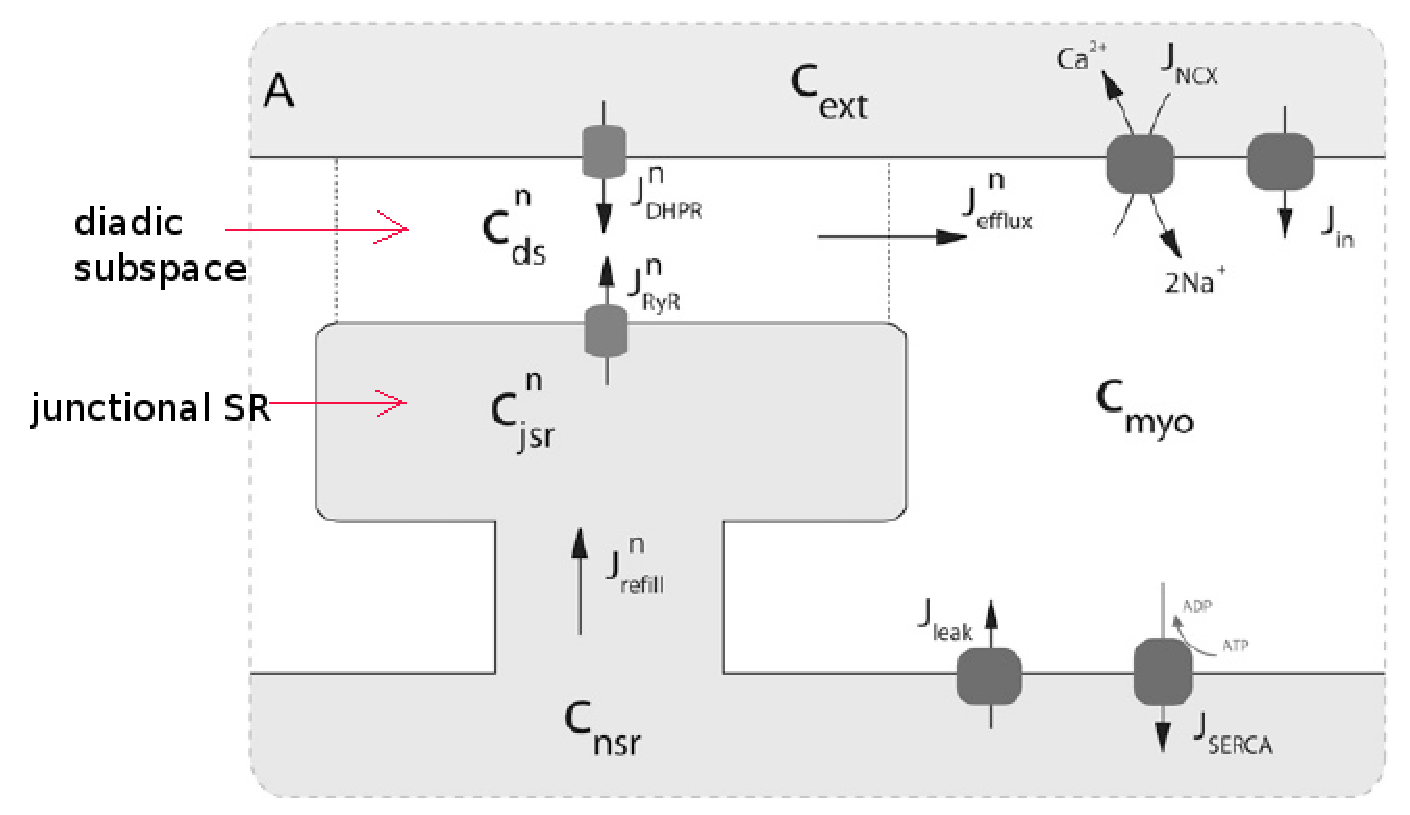
\includegraphics[height=5cm]{./images/CaRU.eps}}
  \caption{The schematic diagram of a CaRU in cardiac cells}
  \label{fig:schematic_CaRU}
\end{figure}

The calcium elevation due to potential depolarization was discussed in
Sect.~\ref{sec:cicr}. However, it was observed that in quiescent
cardiac cell, when there is no potential change, they still detect the
calcium elevation, yet at a local scale.  The local discrete
elevations in myoplasmic \ce{Ca^2+} arises from the opening of a group
of RyRs as a cluster in SR, is termed
{\bf \ce{Ca^2+} spark}~\citep{Cheng1993Calciumspark}. Since then, there
are many terminologies describing the local calcium
elevation~\citep{cheng2008cs}. Using confocal microscopy with
fluorescence calcium detector, Cheng {\it et al.} was the first to
detect the \ce{Ca^2+} sparks in quiescent rat heart cell, as shown in
Fig.~\ref{fig:calcium-spark}. The fluorescence is generally uniform,
and the discrete regions of increase fluorescence (spark) reflect
spontaneous increase in $[\ce{Ca^2+}]_i$. It is now well established
that \ce{Ca^2+} sparks represent the elementary \ce{Ca^2+} release
events that spatially and temporally summate to produce the global
\ce{Ca^2+} transient during EC coupling.


\begin{figure}[hbt]
  \centerline{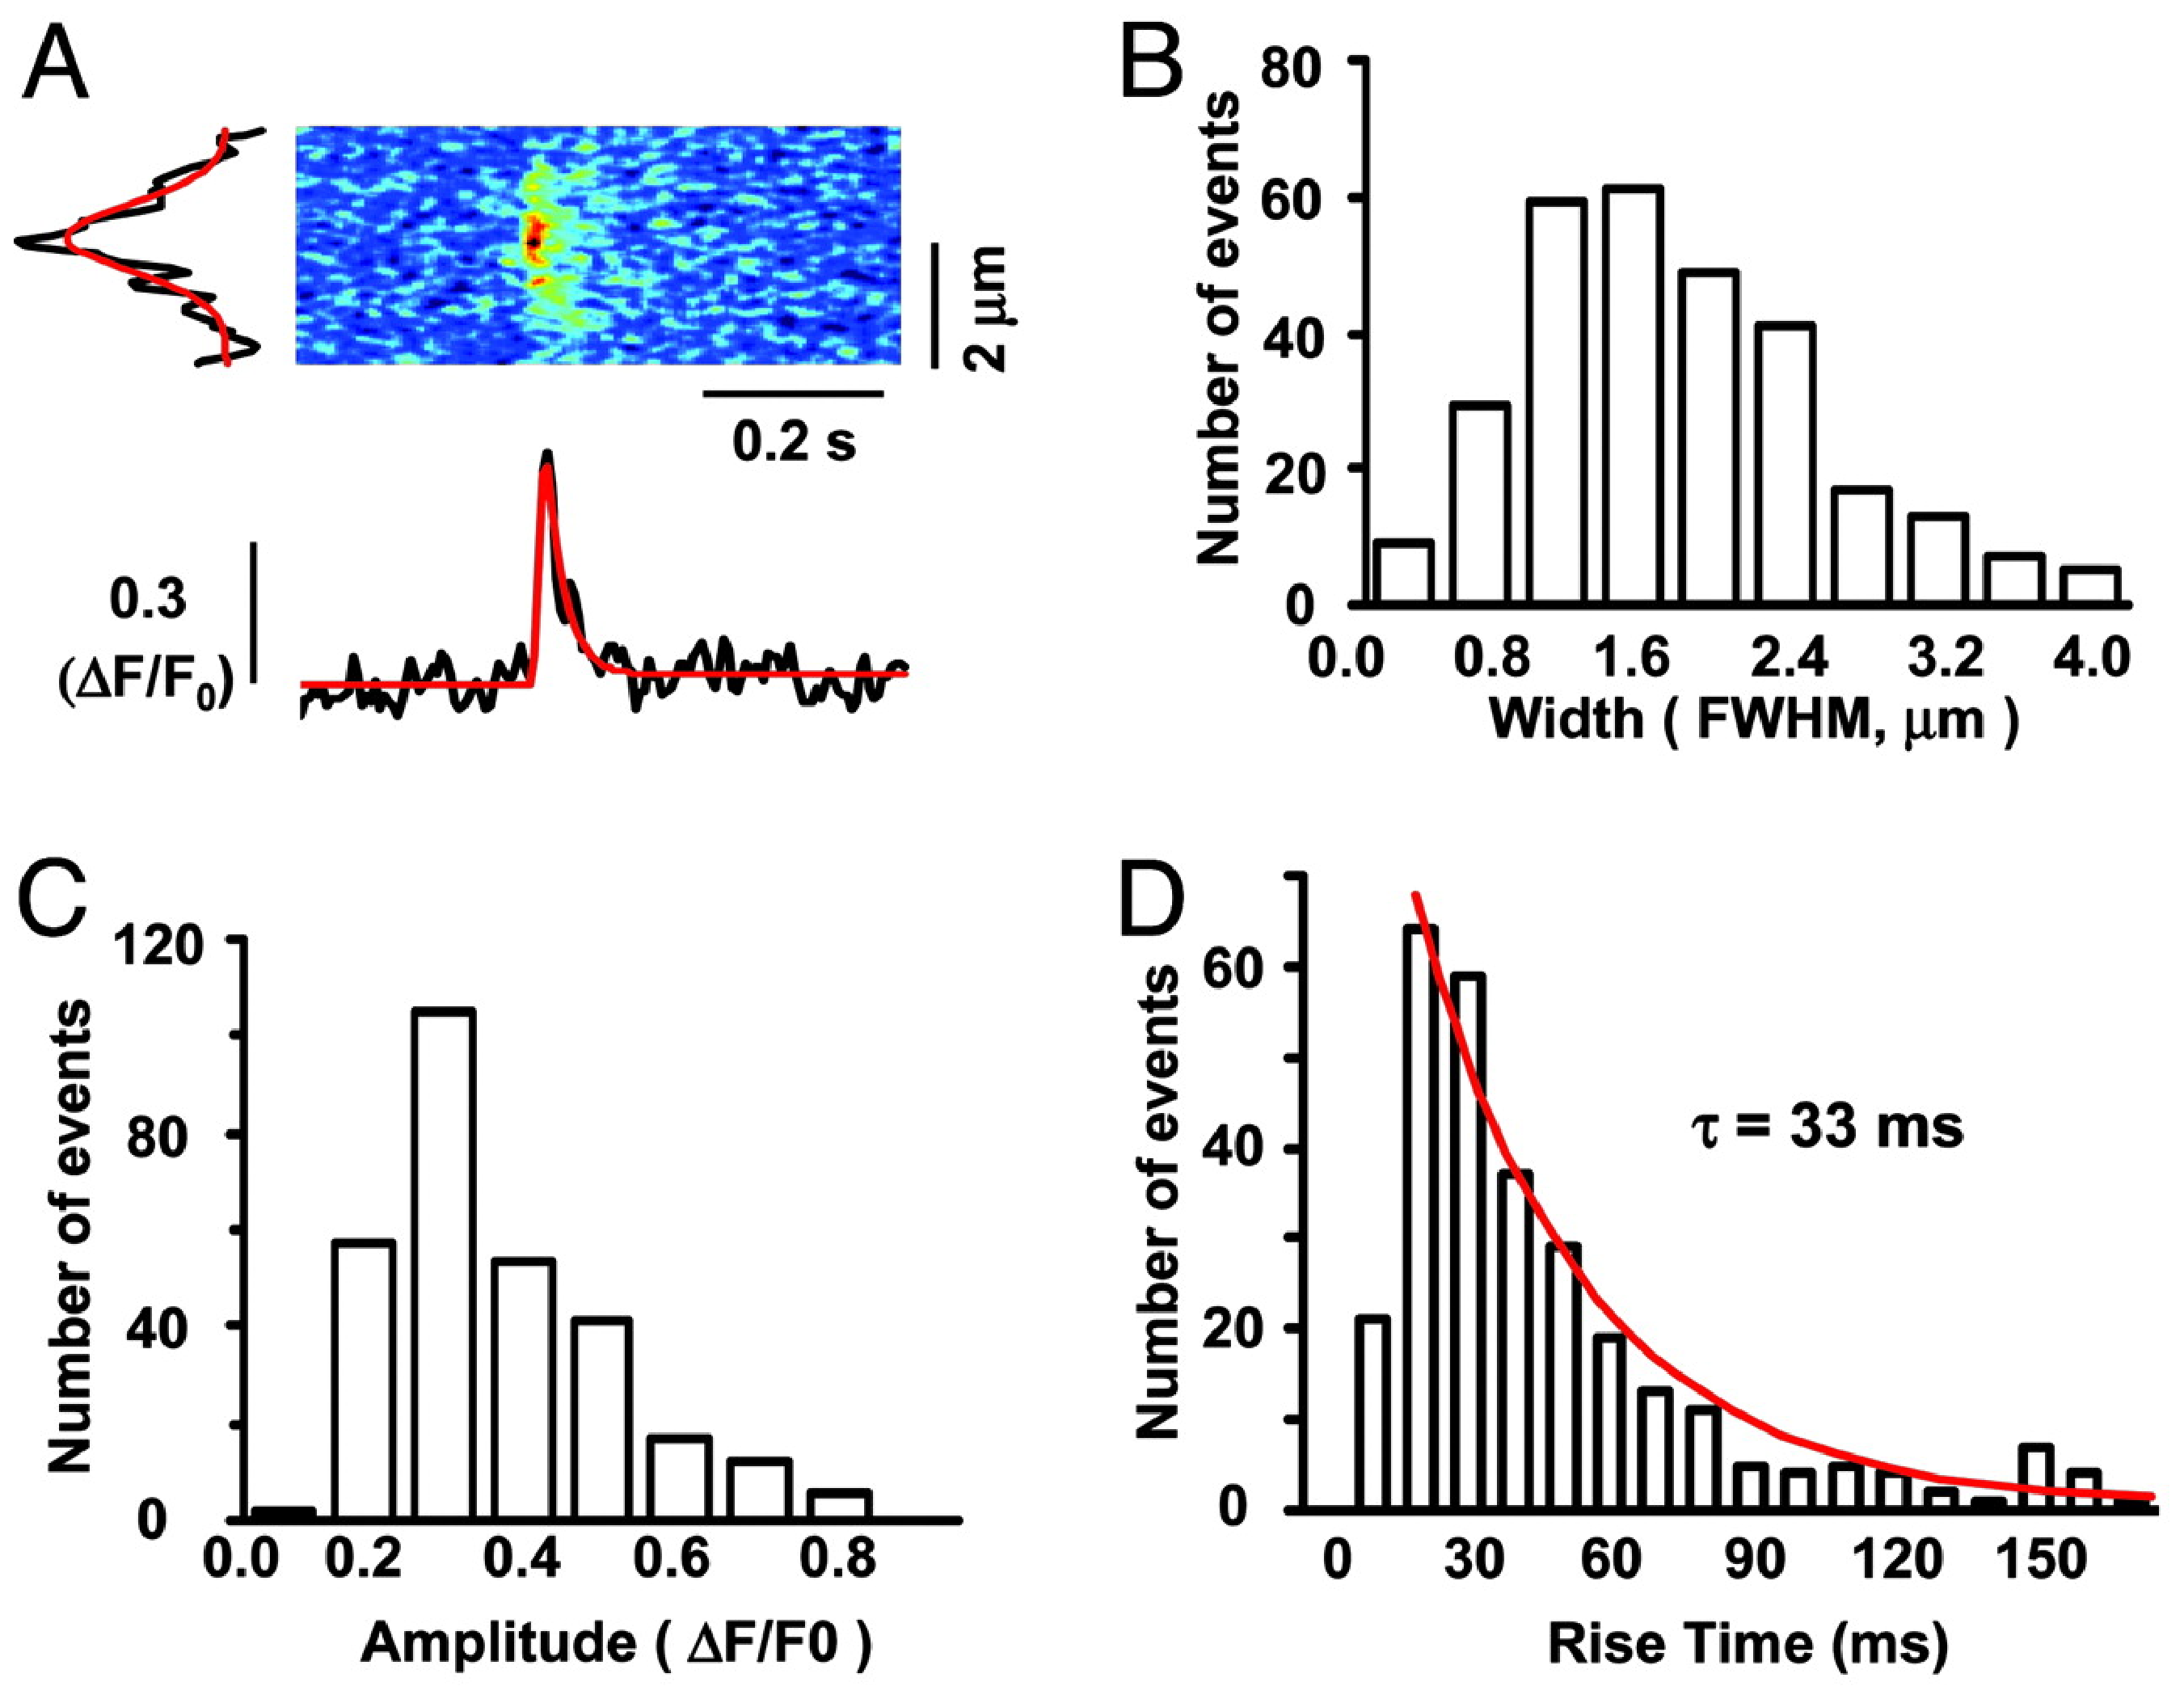
\includegraphics[height=8cm]{./images/calcium_spark.eps}}
  \caption{The color scale denoting the level of calcium
    concentrations (A) a typical \ce{Ca^2+} spark obtained with 1mM
    caffeine; (B-D) histograms of: (B) spark amplitude, (C) spark
    width, (D) of release duration from the onset to the beginning of
    the decay, the red curve is its exponential fit with time constant
    $\tau=33.2$ms}
  \label{fig:calcium-spark}
\end{figure}

Due to its intrinsic positive feedback, the more [\ce{Ca^2+}] to be
released, the more number of RyR channels to open.  Even though within
a {\bf couplon} (e.g. junctional SR + T-tubule), \ce{Ca^2+} release is
a positive feedback, the fractional SR \ce{Ca^2+} release is only
about 50-60\%~\citep{bassani1995fsr}.
\textcolor{red}{There are still debates on the hypotheses of spark
  termination, yet experimental results suggested that there is a
  \ce{Ca^2+}-dependent negative feedback that inactivate RyR channels,
  e.g. calmodulin (CaM)}.
This will be discussed in details in the following paragraphs.
% This local increase in the concentration of intracellular calcium, to
% be precise, it is the increase in concentration of free \ce{Ca^2+},
% excluding calcium bound to buffers or other calcium-binding particles
% .

\begin{figure}[htb]
  \centerline{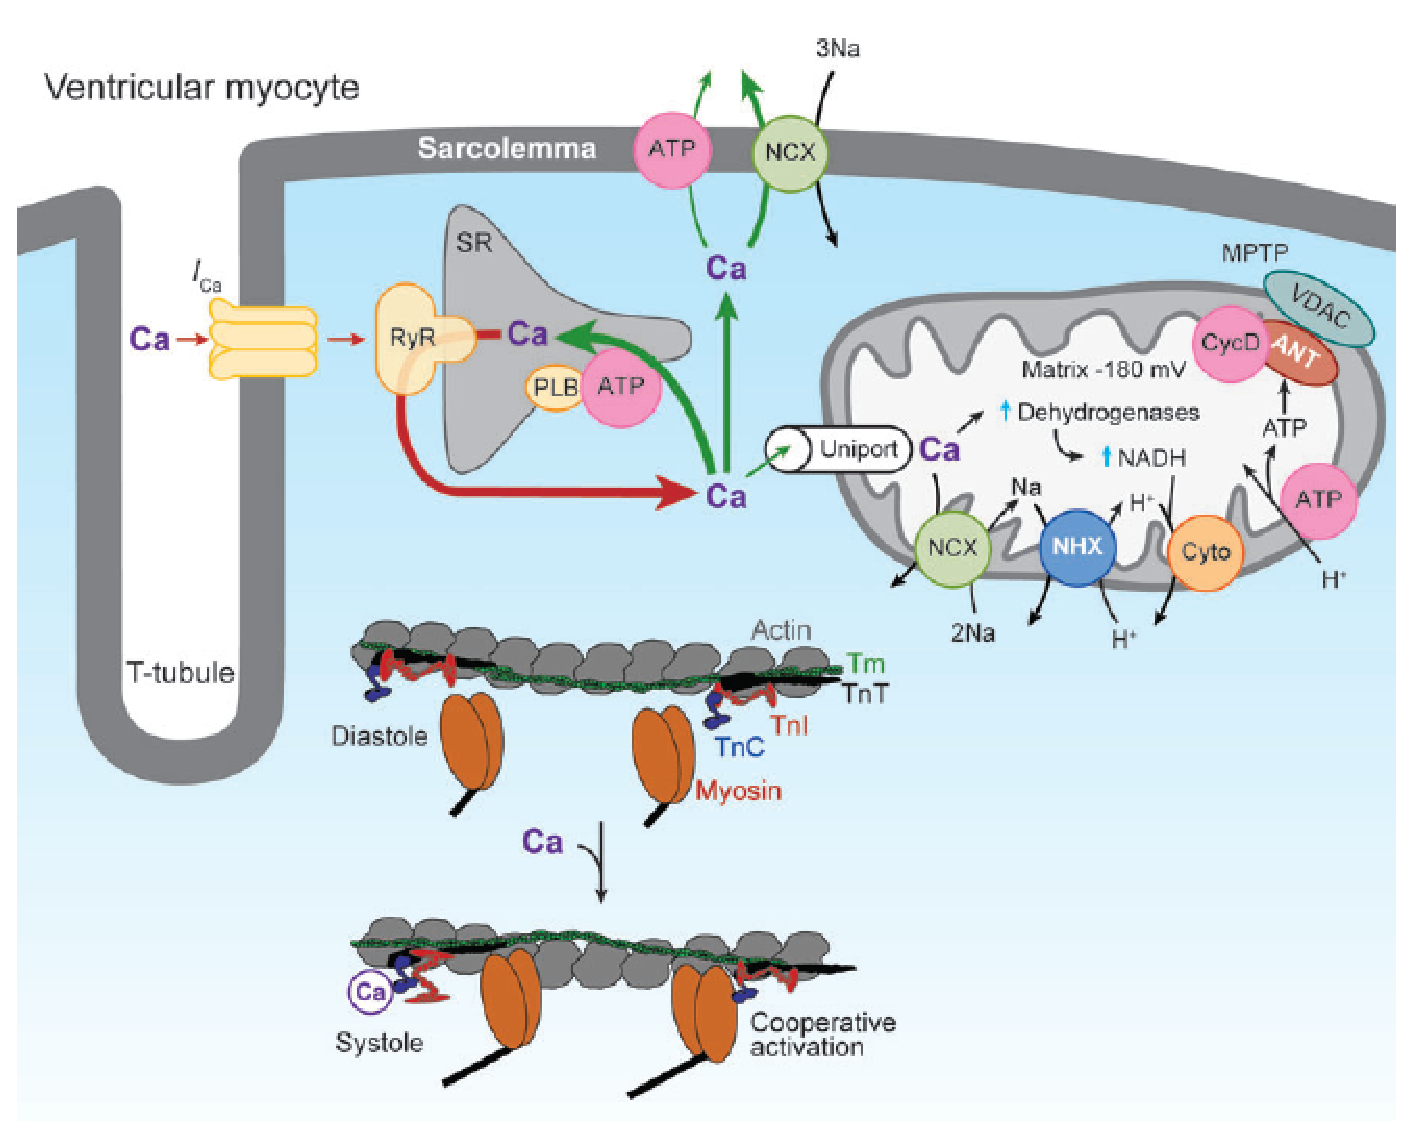
\includegraphics[height=10cm]{./images/Ca_transport.eps}}
  \caption{\ce{Ca^2+} transport}\label{fig:Ca_transport}
\end{figure}

\begin{framed}
  
  {\bf SUMMARY}: In essence, CICR is a mechanism of spontaneous
  calcium release from muscle's {\it sarcoplasmic reticulum} (SR)
  through RyR channels triggered by the low-level entry of \ce{Ca^2+}
  from the extracellular environment via DHPR, as shown in
  Fig.~\ref{fig:Ca_transport}. It then magnify the \ce{Ca^2+} release
  from internal stores, which contributes about 50-90\% of \ce{Ca^2+}
  to the global \ce{Ca^2+} transient~\citep{bers2001ecc}. This
  mechanism regulates the EC process ~\citep{bers2008cca}.  CICR is
  mediated by two well-defined calcium channels: dihydropyridine
  receptors (DHPRs) and ryanodine receptors (RyRs). DHPRs act as
  voltage sensors on the T-tubules, while RyRs are the calcium
  release channels of SR.
\end{framed}


In rat heart cell, there are about $10^6$ RyRs per cell in which
$10^5$, about $10\%$, can be surveyed simultaneously. The opening rate
for a RyR at resting is extremely low ($0.0001$s$^{-1}$).  As a
result,
\textcolor{red}{there are only about 100 sparks/second in whole cell
  at rest}.
Each \ce{Ca^2+} spark leads $[\ce{Ca^2+}]_{ds}$ to 200-300nM,
compared to resting value $100$nM, with half-time decay
($\tau_{1/2}=24.5 \pm 1.86$ms, $n=20$). The requirement for a wave
started is to have a ``macrospark'' of 500nM in calcium
elevation. This is believed the result of many neighboring \ce{Ca^2+}
sparks.  Hence, local calcium elevation via CICR cannot trigger global
\ce{Ca^2+} release.

Under calcium overload condition (i.e. $[Ca]_{SR}$ overload, by
increase $[Ca]_o$ to 10mM), it is observed an increase in RyR's
opening rate around 4-fold ($402\pm 83\%$, $n=9$ with $n$ is the
number of release site). This suggests that
\textcolor{blue}{the spontaneous release of \ce{Ca^2+} is due to RyRs
  become more sensitive to an increase in \ce{Ca^2+} during \ce{Ca^2+}
  overload}.
\textcolor{red}{This is known as RyR adaptation, and still being
  investigated to create a precise RyR model}.

\begin{framed}
  \textcolor{red}{A normal spark is [\ce{Ca^2+}] in the range
    200-300nM}. However, the initiating spark in the wave of elevated
  intracellular \ce{Ca^2+} propagated (at speed of $70\mu$m/s) is a
  macrospark with [\ce{Ca^2+}] about 500nM. This large initiating
  spark may be the result of a summation of several closely spaced
  individual sparks.  The wave appeared as an inverted
  ``V''\citep{Cheng1993Calciumspark}. 
\end{framed}

The flux $J$ of \ce{Ca^2+} associated with a spark is computed as
\begin{equation}
  \label{eq:201}
  J = B.\Delta [\ce{Ca^2+}]_i.V.T^{-1}
\end{equation}
with $B$ is the buffering power of the cell $B=\frac{\text{release
    \ce{Ca^2+}} [\mu M]}{\text{increase  \ce{Ca^2+}} [\mu M]}$,
$\Delta [\ce{Ca^2+}]_i$ is the concentration change during the spark,
$V$ is the volume occupied by the spark, $T$ is the time taken for the
rise of spark. Experimental results gave us $V \approx 10fl, T\approx
10ms, \Delta [\ce{Ca^2+}]_i\approx 0.2\mu M, B \approx 100$, then
$J\approx 2\times 10^{-17}$ mol/s (with $I_{Ca,L}=4pA$).

In its simplest form, CICR is the ``all-or-nothing'' process, i.e. all
RyR channels are either open or closed fully, and all DHPR are either
open or closed fully. In {\it vivo}, however, CICR smoothly
graded. Hence, \ce{Ca^2+}-dependent inactivation is an essential
negative control mechanism that counters the positive feedback of
CICR~\citep{gyorke1994cdnc}. Such phenomenon, however, was not observed
under steady-state conditions or single-channel studies. This is
possible that a regulatory subunit was lost during RyR isolation or
that steady-state studies were inappropriate to describe the transient
phenomenon.

\begin{figure}[hbt]
  \centerline{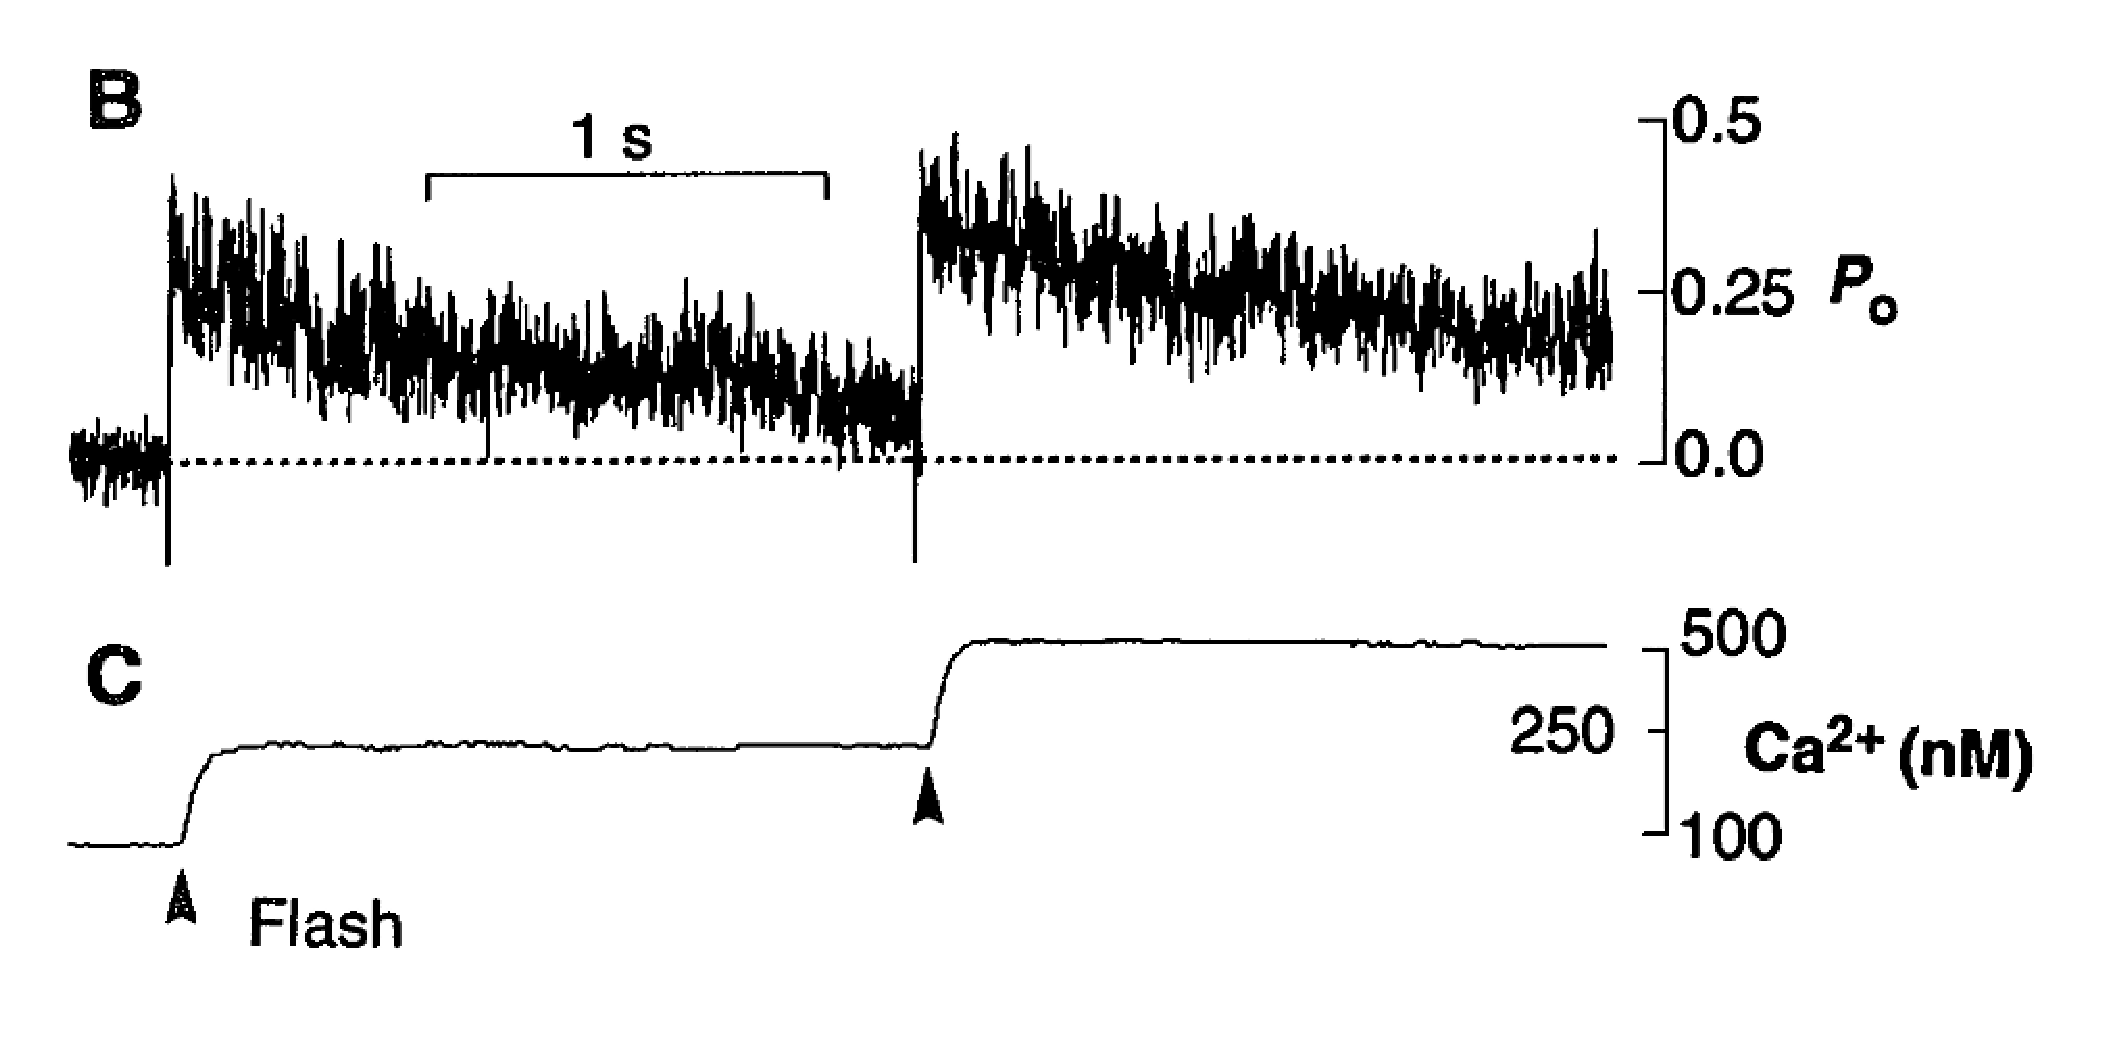
\includegraphics[height=5cm]{./images/RyR_response.eps}}
  \caption{(B) The decrease in opening probability due to prolonged
    \ce{Ca^2+} exposure,(C) activation of RyR channel by two incremental
    increase in \ce{Ca^2+}}
  \label{fig:RyR_response}
\end{figure}

There are various computational models shown that with a precise
adjustment in the \ce{Ca^2+} sensitivity of the \ce{Ca^2+} release
mechanism, it is possible to obtain graded control of CICR. This will
be the topic in another book (Computational Cell Biology).

After the systolic phase, the \ce{Ca^2+} need to be quickly extruded
out of the cell. The two concurrent mechanism to pump the blood out of
the myocyte is Na/Ca eXchanger (NCX) and plasma-membrane
\ce{Ca^2+}-ATPase (PMCA). 

% \section{The role of \ce{Ca^2+}}
% \label{sec:calcium-ions}

\section{Calcium blinks}

$\Ca$ blinks refer to the rapid, substantial decreases in luminal
$\Ca$ release from the junctional SR, a nanometer-sized $\Ca$ stores
(Sect.\ref{sec:calcium_blink}).

\section{Calcium scraps}

$\Ca$ scrap refers to the transient falls of global $[\Ca]_\sr$ which is
coincides with the electrically evoked cytosolic $\Ca$ transient. This was found
in rabbit ventricular myocytes \citep{shannon2003cs}. 

\section{Calcium transient refractoriness}

In cardiac cell, release of $\Ca$ from the SR for the activation of
contraction occurs through the activation of RYRs. This is the global summation
of numerous elementary $\Ca$ events, known as $\Ca$ sparks. The mechanism for
activation is well-known through the process of calcium-induced calcium release
(CICR). 

After a spontaneous calcium spark event, a subsequent stimulated SR $\Ca$
release was added at different time-delay (recovery time). The level of the
second stimulated SR $\Ca$ release increased with the amount of recovery time,
and eventually approaching the original level of the spontaneous release
\citep{cheng1996csc}, Fig.\ref{fig:refractoriness_SRrelease}. Some models assume
RyR2 switch to inactivated (refractory) 'non-conducting' states after opening
is the dominant factor \citep{snyder2000mmc}. Others assume that restoration of
the SR $\Ca$ load is the major factor in time-dependent recovery of SR $\Ca$
release.

\begin{figure}[hbt]
 \centerline{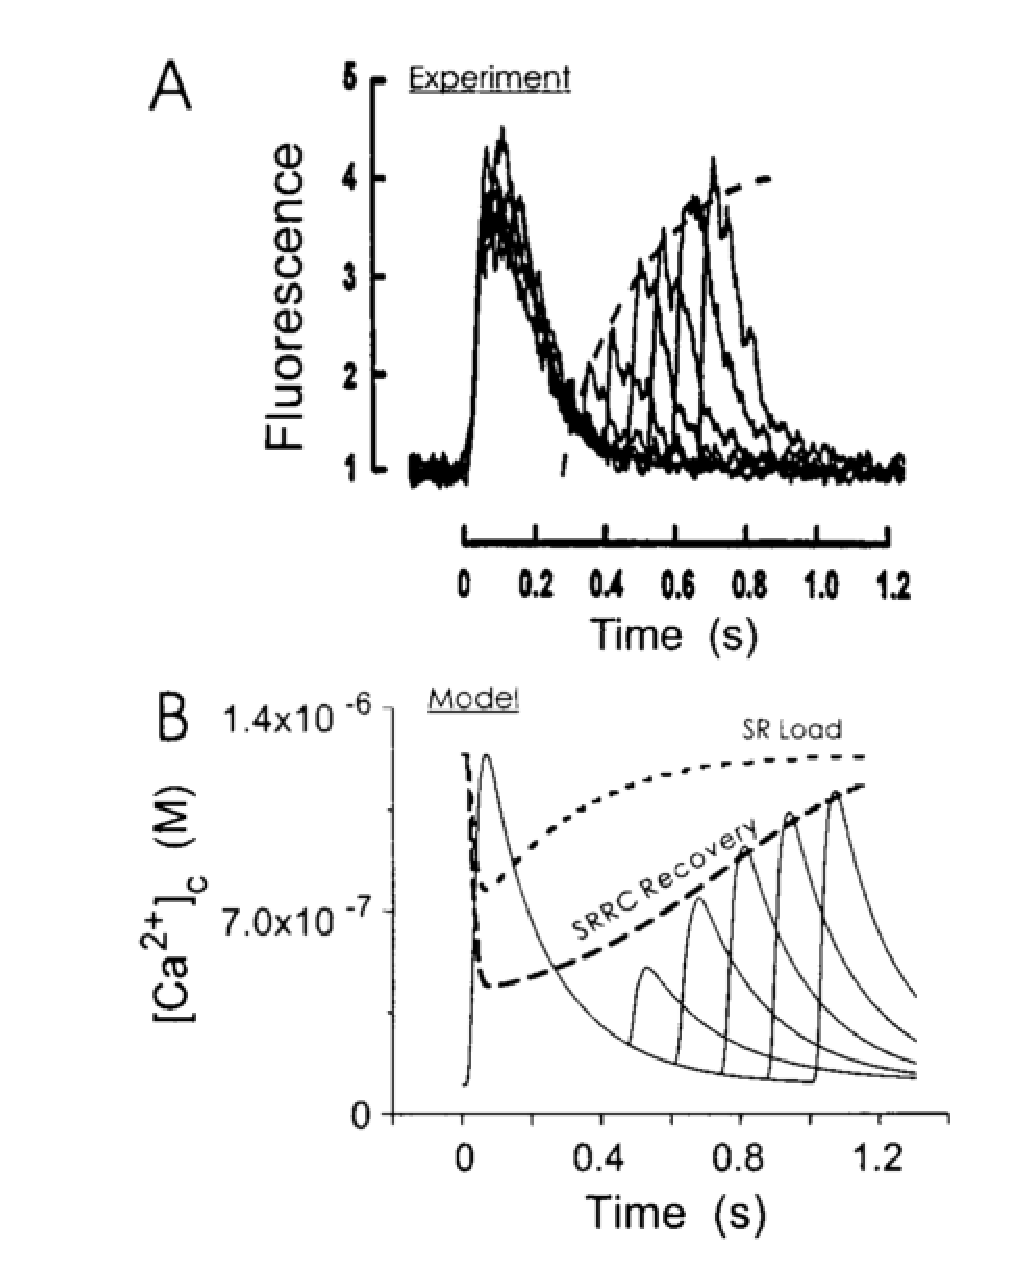
\includegraphics[height=4cm,
 angle=0]{./images/refractoriness_SRrelease.eps}} 
 \caption{(A) Time-dependent recovery of SR $\Ca$ release \citep{cheng1996csc},
 (B) Simulated result \citep{snyder2000mmc}}
\label{fig:refractoriness_SRrelease}
\end{figure}

Under global calcium transient, similarly to spark refractory, the cell is not
available for the next stimulus. Relaxation of cardiac muscle requires both the
terminatio of $\Ca$ release, and the activation of transporters to remove $\Ca$
from the cytosol. A large body of experimental evidences suggested that one or
more mechanism involved in the termination and leading to {\bf refractoriness}
of the CICR.
During the {\bf refractory period}, it's impossible that a new calcium transient
can be triggered. The different proposed hypothesis
\begin{enumerate}
  \item Recovery of the L-type channels from inactivation. However, the recovery
  time for LCC should only require about 300ms \citep{mokelke1997}
  \item Diffusion of SR $\Ca$ from uptake regions to a release region
  \citep{bers1991ecc}. However, the diffusion typically take about 1ms
\end{enumerate}
These hypotheses are not correct, as the experimentally observed  half-time for
recovery of SR $\Ca$ release were $> 400$ms \citep{cheng1996csc}. So, the
recovery here should be explained by the summation of $\Ca$ sparks.

\section{Calcium waves}
\label{sec:calcium-waves}

$\Ca$ sparks are typically independent of each others. However, the $\Ca$ ions
release during a spark from one CRU diffuse and may trigger the spark in the
neighboring CRUs in condition of elevated SR $\Ca$ load. This leads to a
phenomenon known as $\Ca$ waves. $\Ca$ waves refer to the propagation of calcium
elevation inside the cell.
They have been observed in different cell types with speed $\sim 100\mu$m/s,
e.g.
skeletal~\citep{endo1970}, cardiac muscle~\citep{fabiato1972}, medaka
eggs~\citep{ridgway1977}, and astrocytes~\citep{cornell-bell1991}.
\citep{engel1995} measured video imaging of Fluo-3 giving the result of $\sim
260$ ms. This suggested the rise time of $\Ca$ waves is much slower than rise
time of $\Ca$ sparks (about 10-40ms). \citep{lipp1994} measured the propagation
velocity was $\approx 65 \mum/$sec. \citep{parker1996csi} reported the speed to
be 230$\mum$/sec, about twice as fast as that reported by \citep{cheng1996csc}.

In cardiac atrial cells, where lack the universal distribution of
T-tubules, $\Ca$ waves from the sarcolemma to the cell's center is
important for activating myofibrils. In cardiac ventricular cells,
thanks to the deep invagination of T-tubules, near homogeneous calcium
transient can be achieved without needing calcium waves. Thus, in
cardiac ventricular cells, $\Ca$ waves are not physiological and are
believed to be a pathological manifestation of $\Ca$ overload, and
might trigger arrhythmia~\citep{lakatta1993}.

\begin{framed}
  The scattering distribution of CaRUs in the ventricular myocytes
  ensure a nearly spontaneously activation of all CaRUs during the
  AP. However, the uncoupling between neighboring CRUs ensures the
  reliability of the CICR system by a steep gradients of $[\ca]_i$ away
  from the microdomains, and by means of relative insensitivity of RyRs.
\end{framed}

Under certain pathological conditions (often related to an overload of
SR $\Ca$ content or extracellular $[\Ca]_o$), the local control can be come
unstable that allow triggering oscillatory $\Ca$  signals in cardiomyocytes
which may underlies arrhythmias~\citep{katra2005,venetucci2008} or ventricular
fibrillation~\citep{lakatta1993} (Sect.~\ref{sec:ventr-fibr-vf}). Even though
$\Ca$ sparks are found at the site of $\Ca$ waves, an increase in $\Ca$ spark
frequency (by applying low ryanodine concetration) was, by itself,  unable to
trigger $\Ca$ waves. So, there must be other factors, that changes the  spark
property (e.g. the spatial, temporal profile), but not the frequency. 

\citep{cheng1996csc} found that when $[\Ca]_o$ increased from 1 to 10 mM, the
fidelity for $\Ca$ waves increases (from 20\% to 90\% of cells found waves with
the rate 1 to 6 waves/min), and the frequency of spontaneous $\Ca$ sparks
increase $\sim 4$-fold (in a linescan image, from 0.73$\pm$0.1 s$^{-1}$ to
2.96$\pm$0.5 s$^{-1}$), whereas the spark  amplitude increases 4.1-fold (F/F0
from 1.8 to 2.12) and spatial size increases  1.7-fold (FWHM from 1.98$\mum$ to
3.38$\mum$); and propagating $\Ca$ waves was observed.
The duration is alonger with half-time decay of the spark from 23.8$\pm$ 0.97
(ms) to 37.2$\pm$2.15 (ms). Elevated SR $\Ca$ content during $\Ca$ overload will
lead to more $\Ca$ being released (by law of mass action) during  $\Ca$  sparks.
However, the situation is more complex. The high SR $\Ca$ content also modify
the $\Ca$ sensitivity of RyR, thus altering RyR  gating, i.e. less $\Ca$
sensitive on store emptying, and more  sensitive during $\Ca$ refilling. As a
single line-scan image which examined only $\sim 1\%$ of the cell, it's
impossible to know where the wave is initiated. By using a large number of
line-scan images ($> 1000$), they found that $\Ca$ sparks occur near the site
of wave initiation, Fig..

\begin{figure}[hbt]
  \centerline{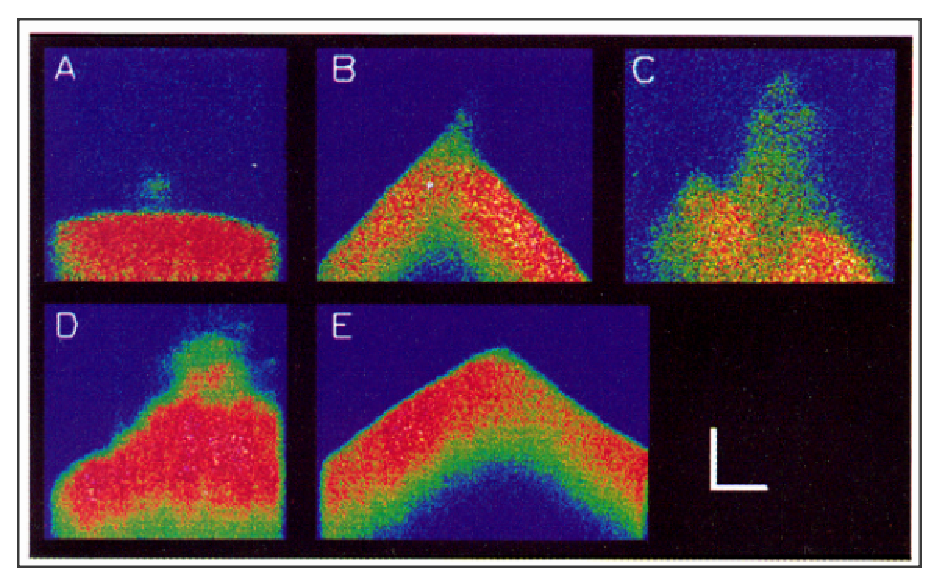
\includegraphics[height=5cm,
    angle=0]{./images/ca_wave_cheng96.eps}}
  \caption{5 examples of wave initiation. $\Ca$ sparks or macrosparks can be
  identified before or at the point of $\Ca$ wave initiation (the apex of the
  inverted ``V''). No spark found in (E), but the apex is more rounded. Scan
  bar: horitonzal 5$\mum$ for (A)(D), and 10$\mum$ for (B),(C),(E); vertical
  200ms\citep{cheng1996csc}}
  \label{fig:ca_wave_cheng96}
\end{figure}



So, the $\Ca$ overload would inevitably affect both CICR system, in
terms of diffusional dissipation of the released $\Ca$, and the $\Ca$
sensitivity of RyR. So far, most conditions leading to arrhythmias are
associated with $\Ca$ overload (e.g. intoxication with cardiac
glyocides, ischemia/reperfusion injury).


\begin{framed}
  
  The local control would fail due to 2 following reasons:
  \begin{itemize}
  \item the local $\Ca$ transient during a spontaneous spark is high
    enough to trigger CICR from the neighboring CRU
  \item the sensitivity of RyR toward cytosolic $\Ca$ uprising could
    increase the $P_o$ where even the small elevation of cytosolic
    $[\ca]_i$ become sufficient to initiate CICR in neighboring
    sarcomeres 2$\mu$m away. 
  \end{itemize}
\end{framed}


Recent discovered mutations in RyR~\citep{}
and CSQ~\citep{}
can lead to change in $\Ca$ sensitivity, i.e. increase $P_o$ of RyR,
independent of $\Ca$ overload. It means that change in RyR gating
induced by mutation are {\it per se} sufficient to trigger
arrhythmias, whether $\Ca$ overload is present or not. This kind of
arrhythmias is known as {\bf CPVT} (Sect.~\ref{sec:cpvt}), which
develop in patients with mutated RyRs during physical exercise or
stress only.

However, the question is
\textcolor{red}{whether alteration of RyR gating from mutated RyR
  alone is sufficient to trigger spontaneous $\Ca$ {\bf waves} causing
  arrhythmias?}.
Based on~\citep{venetucci2007}, the answer is NO; and it need a
certain level of SR $\Ca$ content. What they did is that sensitizing
the RyR by applying a low concentration of caffeine, which can't keep
the $\Ca$ waves over a long period of time. The explanable reason is
that when more $\Ca$ is realised causing the wave, the reduced SR
$\Ca$ load may in turn result in less $\Ca$ being released, which also
desensitize the channel, and eventually stopping the wave. However,
when SR $\Ca$ content was elevated by applying isoproterenol (ISO),
and stimulating the $\Ca$ uptake by phosphorylation of phospholamban
(PLN), the waves are continued to be generated. This can confirm the
important role of $\Ca$ overload to arrhythmias.

\textcolor{red}{So, reducing $\Ca$ load can be a good way to reduce
  the risk for arrhythmias caused by sensitized RyRs}.
Current treatment for sensitized RyRs, by enhancing SERCA pumps may bear certain
risks, as it may increase SR $\Ca$ content too much. An alternate, and better
way is to reduce SR $\Ca$ leak~\citep{wehrens2004nta}.  In order to do that, we
need to know the mechanism of the leak~\citep{Bellinger2008}
(Sect.\ref{sec:calcium_leak}), and the simulation of the cell with 3D distribution of
CaRUs (Chap.~\ref{chap:3d-whole-cell}).

DETECT $\Ca$ WAVES: cross-correlation method was used to calcualte the position
of $\Ca$ waves \citep{cheng1996csc}. The fluorescence profile of the wave at a
selected scanline is chosen as the reference waveform V. The cross-corelation R
between this reference waveform and another linescan W is calculated as
\begin{equation}
R(x) = \int_u W(x+u)V(u)du
\end{equation}
Then, the position of the wave P on the scan line W was calculated from the
position of the point x that has maximum cross correlation R with the reference
waveform.
\begin{equation}
P: R(P) = max[R(x)]
\end{equation}
This process was applied iteratively. After each run, the scan line W is aligned
by using the maxima of the cross-correlation max[R(x)] as the reference point;
and the new reference waveform is selected by averaging the aligned scanline.
The algorithm converges after 4 to 8 iterations, after which we have the
position of the wave as the function of time, the averaged spatial profile of a
wave, as well as the average time course of the $\Ca$ wave (at a point in cell). 
NOTE: The quantitative data analysis was performed with means$\pm$ SE,
independent or paired T-test was applied with  $P$-value $< 0.05$.


More references:
~\citep{berlin1989}

\section{Diastolic $\Ca$ leaks}
\label{sec:calcium_leak}
 
The amount of $\Ca$ within the sarcoplasmic reticulum (SR) play a central role
in cardiac $\Ca$ signalling.  Congestive Heart Failure (HF) is a condition
characterized by reduced contractility of the heart muscle \citep{hasenfuss2002,
sjaastad2002}. In such conditions, there are many changes in cardiac cells, e.g.
lower SERCA pump activity, smaller influx $I_\ca$ (which cause lower gain of
release), anomalous activity of NCX, higher SR $\Ca$ leak. However, the relative
importance of these changes are still debated \citep{bers2003, marks2003}. The
contractile dysfunction is hypothesized as the result of calcium leak from SR in
the heart cells where the RyR hyperphosphorylation can result into the loss of
SR $\Ca$ content \citep{wang2005ecc}. Patients with HF suffer from arrhythmias
that are thought to be related to improper $\Ca$ handling and are generally associated with
increased rather than decreased SR $\Ca$ load, i.e.
$\Ca$ overloaded arrhythmias. In particular, excessive level of $\Ca$ in the SR
can cause regenerative release of $\Ca$, which have been found to be a
surpressor leading to arrhythmias \citep{lederer1976, kass1978, berlin1989,
cheng1996csc}. However, the mechanism and pathway of calcium leak was unknown.
The concept of $\Ca$ leak is broadly defined as the loss of $\Ca$ from SR under
resting or quiescent conditions.

Different mechanisms have been proposed to explain this leak:
\begin{enumerate}
  \item The major and visible pathway of $\Ca$ leak during relaxation is
  spontaneous $\Ca$ sparks \citep{bers2001ecc}.
    
  \item The backflux via SERCA pumps \citep{shannon1998, shannon2000rms}.
  However, recent studies believed that reversed mode do not happen at
  physiological level of $\Ca$. 
  
  \item Some believed the existing of ``leak'' channels\citep{camello2002,
  shannon2000rms}. \citep{shannon2000rms} used SR leak constant 0.0047-0.0004
  per sec. 
   
  \item the leak is from ``rogue'' RyRs (or non-junctional RyR). These RyRs have
  not been visualized directly, but their existence is suggested
  \citep{lipp2002}. Rogue RyRs are different from RyRs in ``corbular'' SR which
  are also clustered, but are not apposed to LCC. From biochemical studies, high
  level of PKA can dissociate FKBP12.6 from RyR, leading to a higher open
  probability of RyR \citep{marks2002, marx2000}. However, in failing heart
  where PKA is over-expressed due to hyperactivity of beta-adrenergic receptor
  \citep{ono2000}, the leak increase but failed to detect  an increase in spark
  rate \citep{gomez1997}. A sound explanation is that, in HF, the decrease
  activity of SERCA and increase activity of NCX would lead to decreased SR
  $\Ca$ load which leads to a decrease in spark rate. However, even when SR load
  was made the same as in control conditions, \citep{li2002} didn't see the
  increase in spark rate. So, the question is from which source the leak come
  froms? One study showed that under over-expression of FKBP12.6, which
  stabilize the closing of RyRs, the leak is decreased \citep{prestle2001}. So,
  the non-spark leak was hypothesized  to be caused by unclustered RyR
  (non-coupled RyRs) located far away from SR-T-tubule junctions
  \citep{sobie2006}.

  \item the disruption in the coupling between RyRs in the cluster, which may
  destabilize the $\Ca$ release system \citep{sobie2006}.
  
  \item the invisible (or silent of loss) pathway of $\Ca$ leak from non-spark
  events of junctional RyRs \citep{williams2011}. This leak is from an
  undetectable non-spark events, i.e. the opening of one or a few RyR channels.
  In this study, the leak from rogue RyRs is non-significant.
  
  
\end{enumerate}

Non-sparks events have been described in skeletal \citep{shirokova1997}, cardiac
\citep{lipp2002} muscles, and cardiac vesicles \citep{shannon2005}. However, its
physiological meaning, nor the extent of its contribution to $\Ca$ leak has not
been fully studied. \citep{bassani1995rdc} estimated it's about 0.2$\muM$/sec in
rabbit and 0.32$\muM$/sec in rat (where SR is dynamics), which is comparable
with the release by $\Ca$ sparks 0.2-0.8$\muM$/sec (estimated at that time).
\citep{lukyanenko2001} estimated diastolic leak flux of about $J_\leak \approx
5-30\muM$/sec, which is consistent with SR leak flux 18$\muM$/sec derived by
\citep{balke1994}. This value, however, is much higher than the value estimated
by \citep{bassani1995rdc}. This is ascribed by the fact that the later
experiment was done when SR $\Ca$ was fixed high, while the previous one jSR
$\Ca$ change. NOTE:
\begin{equation}
J_\leak = \frac{i_\spark \times t_\spark \times f}{z_\ca \times F \times V}
\end{equation}
with $f=2-6$events/sec/100$\mum$, the line scan acquisition volume
$V=100\mum^3$, and single spark current $i_\spark=10-20$pA \citep{izu2001}, with
spark duration $t_\spark=5$ms.

\citep{shannon2002} estimated that $J_\leak$ is about 4-15$\mumol/L$ cytosol per
second at physiological $[\Ca]_{SRT}$, which is about 30\% of the total efflux
rate. The other part was ascribed to the reverse $J_\pumpR$. However, backflux
in SERCA is rarely found at normal condition. Recently, \citep{santiago2010}
concluded that non-sparks events are from RyR openings, aka $\Ca$ quarks
(Sect.\ref{sec:calcium_quarks}). NOTE: $\Ca$ embers are not considered as non-spark
events. Diastolic SR $\Ca$ leak is about $6.3\pm 1.1\mumol/$L cytosol/sec.
However, the spark-dependent leak rate is lower, i.e. about 2.64$\mumol/$L
cytosol/sec. Thus, a large fraction of SR $\Ca$ leak should be from non-spark
events.

\begin{framed}
NOTE: 1 sparks per 100$\mum^2$ per second is translated to 3.07 sparks per pL
per second \citep{santiago2010}.
\end{framed}

Recently, \citep{williams2011} using novel computational model, proved
that non-spark calcium leak can be accounted solely through RyR (which account
for of about 40\% of calcium leak, and the other 60\% through detectable
spontaneous $\Ca$ sparks in a resting cell).


To study $\Ca$ leak, LCC can be pharmacologically blocked at $V_m$ of -80mV by
either removing external $\Ca$ \citep{cheng1993cse} or using 100$\muM \Cd$
\citep{cheng1993cse, cannell1995b}.


\section{Calcium buffers}
\label{sec:buffers-calcium}
\label{sec:calcium-buffers}

The sustained high level of calcium can be toxic to the cell. Even though the
total calcium is high, the level of free calcium is kept at very low thanks to
endogenous buffers. Here, the term {\bf buffer} is restricted to the context of
chemical species that act as ligands for $\Ca$. Examples of endogenous $\Ca$
buffers:
\begin{itemize}
\item large size:
  \begin{enumerate}
  \item Troponin C (immobile buffer) - Sect.\ref{sec:troponin}
  
The contractile regulatory protein: in
  the myoplasm. There are two high-affinity binding sites, and two low-affinity
  binding sites for each Trpn-C.
 
  \item Calsequestrin : in the junctional SR (jSR) - Sect.\ref{sec:calsequestrin}
  high-capacity, low-affinity
  
  \item SL buffers: very large buffer capacity ($> 1$mM)
  \item SR buffers:
  
  \item calexcitin (neuron-specific): interacts with proteins that control the
  firing state of neurons such as inhibiting $\Vm-$dependent $\K$ channel
  
  \end{enumerate}

\item smaller size:
  \begin{enumerate}
  \item Calmodulin - Sect.\ref{sec:calmodulin}
  \item ATP (mobile buffer) - Sect.\ref{sec:ATP-molecule}
  \item parvalbumin (less mobile) - Sect.\ref{sec:parvalbumin}
  \item SERCA pump (immobile buffer) - Sect.\ref{sec:SERCA_pump}
  \end{enumerate}
  
\item Calbindin - Sect.\ref{sec:calbindin}
\end{itemize}

There are so-called exogenous buffers that are artificially injected into the
cell to help measuring ionic concentration. These exogenous buffers, however,
may changes the dynamics of the ion in relative to the {\it in vivo} condition.
\begin{itemize}
    \item Calcium indicator (dyes - Sect.~\ref{sec:fluorescence-dyes})
\end{itemize}

In skeletal muscle, the most important $\Ca$-binding proteins are:
troponin (attaching to the thin filament), parvalbumin (a soluble
protein found in high concentrate in myoplasm of some muscles), and
calsequestrin (a low-affinity but high-capacity $\Ca$-binding proteins.
\textcolor{red}{Binding is assumed to obey the law of mass action,
  with one-to-one binding stoichiometry}. 
\begin{equation}
\ce{B + Ca2+ <=>]k^+][k^-] CaB}
\end{equation}
 
\subsection{Dynamics buffering: Stationary vs. Mobile Buffers}
\label{sec:dynamics-buffering}
In living cells, calcium ions are strongly buffered.
The buffer concentration can be from 100-300 $\mu$M in cytoplasm, and higher in
ER/SR.  In chromaffin cells, about 25\% of buffers in cytoplasm with molecular
weights of the order of 15kDa~\citep{zhou1993}. Buffers are classified into 2
types~\citep{wagner1994erb}:
\begin{itemize}
\item stationary (dominant)
\item mobile: e.g. Fura-2 (exogenous fluorescent indicator), BAPTA
\end{itemize}

Let $\Bi$ is the buffer, with $i$ can be $s=$ stationary, $m=$
mobilized. A reaction for the binding of Ca to buffer is given
\begin{equation}
  \label{eq:933}
  \ce{B_i + Ca^2+ <=>[k^+_i][k^-_i] CaB_i}
\end{equation}


Under the assumption of {\bf mass action kinetics} and {\bf Fickian diffusion},
there are 4 variables: [\ce{Ca^2+}], [\ce{Ca^2+B_m}], [\ce{Ca^2+B_s}],
[\ce{Bm}]. Their changes over time can be written in the form of ODEs

\begin{equation}
  \label{eq:934}
\begin{split}
  \frac{\partial [\ca]}{\partial t} &= \text{react\_term}_1() + D_{\ce{Ca}}\nabla^2[\ca]\\
  \frac{\partial [\Bm]}{\partial t} &= \text{react\_term}_2() +
  D_{\ce{B_m}}\nabla^2[\Bm]\\
  \frac{\partial [\ce{CaB_m}]}{\partial t} &= \text{react\_term}_3() + D_{\ce{CaB_m}}\nabla^2[\CaBm] \\
  \frac{\partial [\ce{CaB_s}]}{\partial t} &= \text{react\_term}_4()
\end{split} 
\end{equation}
with $D_\ca,D_{\ce{B_m}}, D_{\ce{CaB_m}}$ are the diffusion coefficients for
free calcium, mobile buffer and Ca-bound mobile buffer, respectively; and
\begin{eqnarray*}
  \text{react\_term}_1() &&= k^-_m[\CaBm]+k^-_s[\CaBs] - ( k^+_m[\ca]
  + k^-_s[\ca]) \\
  \text{react\_term}_2() &&= k^-_m[\CaBm] -  k^+_m[\ca] \\
  \text{react\_term}_3() &&= -k^-_m[\CaBm] +  k^+_m[\ca] \\
  \text{react\_term}_4() &&= -k^-_s[\CaBs] +  k^+_s[\ca] 
\end{eqnarray*}

\textcolor{red}{Eq.~\eqref{eq:934} are the exact form of slow-kinetics
  buffering}. Using the law of conservation and equations above, the total
  calcium concentration in the microdomain is
\begin{equation}
  \label{eq:935}
  \ce{[Ca]_T = [Ca] + [\CaBm] + [\CaBs]}
\end{equation}
then differentiate over time on both side, using eqs.~\eqref{eq:934},
we have
\begin{equation}
  \label{eq:936}
  \frac{\partial[\Ca]_T}{\partial t} = D_{\ce{Ca}}\nabla^2[\Ca] +
  D_{\ce{CaB_m}}\nabla^2[\ce{CaB_m}]
\end{equation}

\subsection{Buffering capacity}
\label{sec:buffer_capacity}

A general parameter, the endogenous calcium-binding ratio $\kappa_s$, is used
to measure and compare the overall capacity of various cells to buffer $\Ca$. It's independent
of the type of $\Ca$ buffer proteins involved.
It's defined as the differential ratio the concentration of
$\Ca$-bound to buffers over free $[\Ca]$.
\begin{equation}
\kappa_s = \frac{d[\CaB]}{d[\Ca]_i}
\end{equation}
So, $\kappa_s$ is a functional measure of the degree of calcium-buffering
capability of a cell \citep{Neher1998}. This values increases when free $[\Ca]$
increases, and then decreases as free $[\Ca]$ exceeds the level that saturate the buffers.

\begin{enumerate}
  \item In hippocampus, the inhibitory interneurons have a two to three times
  larger buffering power (i.e., higher Ks) than the excitatory interneurons, and
  thus are able to withstand larger Ca2+ challenges \citep{lee2000}
  \item In spinal coord, the motor neurons have $\kappa_s = 50$ (i.e. 1 in 50
  calcium ions entering the cells are free, i.e. only 2\% calcium remains free,
  unbound by cytosolic proteins)
  \item In sympathetic superior cervical ganglia (SCG), $\kappa_s$ varies from
  250-500 (depending on value of $[\Ca]_i$)
\end{enumerate}
$\kappa_s$ also change between young and matured cells, i.e. developmentally
regulated. 

When an exogenous buffer is added to the cell, e.g. Fura-2, the buffer strength
$\kappa$ is increased by an amount $\Delta \kappa$ that depends on the amount
and physical properties of the exogenous buffer.
\begin{equation}
\Delta \kappa = \frac{d[\CaB]}{d[\Ca]}=\frac{[\B]_T.K_d}{\left([\Ca] +
K_d \right)^2} = \frac{[\B]_T}{K_d}\left(1+ \frac{[\Ca]}{K_d}\right)^{-2}
\end{equation}
with $[\B]_T$ is the total exogenous buffer B added; $K_d$ is the dissociation
constant of the buffer. 

\begin{enumerate}
  \item At low $[\Ca]_i$, i.e. the calcium-binding ratio can be approximated by
  the ratio of the total buffer $[\B]_T$ over its dissociation constant $K_d$.
  \item When $[\Ca]_i$ approaches $K_d$, $\Delta \kappa$ reaches a
maximum as a function of $K_d$ when $K_d=[\Ca]$ \citep{wang1993lpf}.
\end{enumerate}

\textcolor{red}{Under the assumption either low affinity buffers $[\Ca] \ll
K_{d}$ or $[\Ca]$ change is small enough (relative to basal $[\Ca]$)} then
$\kappa_S$ can be considered constant.  The above assumption of constant
$\kappa_S$ is violated when buffers saturate or the combined signal is larger
than the sum of individual signals (i.e.
supra-additivity). Then $\kappa_S$ is replaced by
\begin{equation}
\kappa' = \frac{\Delta[\CaS]}{\Delta [\Ca]} =
\frac{\text{S}_T}{K_{D,S} \left( 1+ \frac{[\Ca]_1}{K_{D,S}} \right)
\left( 1+ \frac{[\Ca]_2}{K_{D,S}} \right) }
\end{equation}
with $[\Ca]_1, [\Ca]_2$ are values at start of signal and peak value,
respectively. 


With fast buffering is assumed:
$[\CaB]=[\B]_T\frac{[\Ca]}{([\Ca]+K_d)}$.



\subsection{Slow/Fast time scales}
\label{sec:time-scales}
%\subsection{Slow and Rapid bufferings}
\label{sec:slow_rapid-bufferings}

\begin{framed}

The characteristic time (time constant) for buffering can be estimated by
linearizing the terms for the association reaction around their equilibrium values
\begin{equation}
  \label{eq:1095}
  \tau_i = \frac{1}{k^-_i+k^+_i([\Ca]+[\Bi])} \qquad \text{(sec)}
\end{equation}

The characteristic time for diffusion 
\begin{equation}
  \label{eq:1096}
  \tau_\text{diffusion} \approx L^2/D  \qquad \text{(sec)}
\end{equation}
with $L$ is the length profile of the environment with diffusion
constant $D$.

\end{framed}

In the example above, there are 5 different time scales: two for the two
bufferings, and three for the time scales of diffusion.
Typically, the time-scale of chemical reaction occur much faster than the
time-scale for diffusion. \textcolor{red}{Time constant for buffering has been
estimated in the range of 10 ms}, which is about 10x faster than that of
diffusion (as showed in the box). In chromaffin cells, a time constant for
stationary and mobile buffers of the order of 1 ms has been estimated using
patch pipettes (Neher and Augustine, 1992). NOTE: Fura-2 $\Ca$ endogenous buffer
 (Sect.\ref{sec:fura-2}) has $k^-_m = 97$ (sec), and $k^+_m = 601 \muM$/sec,
 i.e. $\tau_i = 5$(ms).


\begin{framed}
  The diffusion constants for unbound $\Ca$ was estimated to be in the
  range 225-300$\mu$m$^2$.s$^{-1}$~\citep{zhou1993}. Suppose the spatial profile
  of $\Ca$ has a length scale of L=5$\mum$, then $\tau_\text{diff}=83-111$ (ms).
  
  The molecular mass of mobile buffers in the range 7-20kDa, and has the
  diffusion constant 2-10 times smaller than that for $\Ca$.
  Diffusion constants for small exogenous buffers, such as BAPTA or fura-2, are
  probably smaller than that of $\Ca$ (Timmerman and Ashley, 1986); thus giving
  an even larger $\tau_\text{diff}$.
\end{framed}

\textcolor{red}{Typically, it's assumed that the buffering is rapid (fast or
instant) w.r.t diffusion}. So, rapid buffering can be assumed in which the [Ca]
is determined by the dissociation and association of calcium with buffer at
equilibrium. By eliminating the shortest time scales, it allows larger time
steps to be used in the simulation.

So, the condition for rapid equilibrium is
\begin{equation}
  \label{eq:1097}
  \tau_i \ll L^2/D
\end{equation}

There are two strategies that can be used with rapid buffer approximation
\begin{enumerate}
  \item linear approximation: Sect.\ref{sec:linear_buffer}
  \item rapid buffer approximation: Sect.\ref{sec:rapid_buffer}
\end{enumerate}

If you want to go with very small time-step in the simulation, then you can
choose to keep the dynamics buffer (Sect.\ref{sec:dynamics-buffering}).

\subsection{Linear approximation}
\label{sec:linear_buffer}

To study the effect of $\Ca$ signaling under the effect of buffering, there are
different approaches. One common is ``single compartment linear model'' which
requires 2 basic assumptions \citep{Neher1998}:
\begin{enumerate}
  \item $\Ca$ is homogeneous inside the compartment (no spatial gradient or
  spatial homogeneity)
  \item $\Ca$ is in chemical equilibrium with its buffers at any momement of
  time.
\end{enumerate}
So, (1) there is no diffusion term in the equation for $\Ca$, and (2) there  is
no need for an ODE representing buffer concentration's dynamics.

The method describe the decay of $\Ca$ in a small cell following the elevation
of calcium, e.g. during AP. Here, the decay of $\Ca$ signal is governed by
combined action of $\Ca$ pumps and other transport mechanisms. The requirements
for the assumption to be valid are (1) $\kappa_s$=constant, i.e. change in
$[\Ca]$ is small relative to the basal level or the buffers are low affinity
(i.e. $[\Ca]\ll K_{d}$), (2) the combined effects of $\Ca$-pumps, leaks and
other transport mechanism are assumed to produce a net $\Ca$ flux which is
proportional to the deviation from steady state (Sect.\ref{sec:buffer_capacity}
for understanding $\kappa_s$).

The increase in calcium $\Delta [\Ca]$ is proportional to the influx of calcium
$\Delta Q_\ca$, and inversely proportional to the total $\Ca$-binding ratio
\begin{equation}
\Delta [\Ca] = \frac{\Delta Q_\ca}{z_\ca.F.V (\kappa_s+1)}
\end{equation}
with $F=$Faraday constant, $v=$accessible volume of the cell, $z_\ca=2$
(valence of calcium). $\kappa_s$ is calculated as given in
Sect.\ref{sec:buffer_capacity}. In the case of buffer saturation, we need to
replace $\kappa_s$ by $\kappa'$.

\begin{equation}
\kappa'_s = \frac{\Delta [\CaB]}{\Delta [\Ca]} = \frac{[\B]_T}{\kappa_s
\left(1 + [\Ca]_1/\kappa_s\right) \left(1+ [\Ca]_2/\kappa_s\right)}
\end{equation}
with $[\Ca]_1$ is the value at the start of the signal, and $[\Ca]_2$ is the
value at the peak of the signal \citep{zhou1993}.

% The $\Ca$-binding
% ratio $\kappa_s$ is defined as the differential ratio of $\Ca$-bound to buffer
% over free $\Ca$.
% \begin{equation}
% \kappa_S = \frac{d[\CaB]}{d[\Ca]}
% \end{equation}

% If the buffering effect of all cellular buffers can be combined, we can assume
% as there is one hypothesized buffering ligand S, and
% \begin{equation}
% \kappa_S = \frac{[\text{S}_T]}{K_{D,S}} \left( 1 + \frac{[\Ca]}{K_{D,S}}
% \right)^{-2}
% \end{equation}
% with $K_{D,S}$ is the dissociation constant. 


\subsection{Rapid buffer approximation (RBA) or rapid equilibrium approximation
(REA)}
\label{sec:rapid_buffer}

Rapid buffer approximation (RBA) or rapid equilibrium approximation (REA) is not
linear theory (Sect.\ref{sec:linear_buffer}). Under REA, the first assumption of
linear approximation, i.e. spatial homogeneity, is abandonded, i.e. there is
different region in the cytoplasm with different concentration of calcium from
that diffusion can occur.
The only assumption is that free $\Ca$ at any time is under local equilibrium
with its buffers \citep{wagner1994erb}.
It means that the validity of REA requires that the time scales for buffering be
rapid with respect to the time scale of diffusion (Sect.\ref{sec:time-scales}).

Even though RBA is not a 'linear' theory, in the context of small signal (for
which the calcium-binding ratio $\kappa_s$ can be considered constant), it can
satisfy the criterion of linearity.


\subsection{-- 1 mobile buffer + 1 stationary buffer: buffering factor}
\label{sec:buffering-factor}

As described above (Sect.\ref{sec:time-scales}), typically, the time scales for
diffusion are slower, so we can assume rapid buffering, i.e. the buffer reaching
equilibrium at any point in space before any appreciable diffusion occurs, to
simply the dynamics description of the buffers. So, instead of solving an ODE,
the calcium-bound buffer concentration can be directly calculated using an
algebraic formula.
\textcolor{red}{Under the assumption of rapid buffering for both stationary and
mobile buffer}, then $\ce{[CaB_i]}$ quickly reach the steady state concentration
or $\frac{\partial [\CaBi]}{\partial t} = 0$. Then we have
\begin{equation}
  \label{eq:937}
  \ce{[CaB_i]} = \frac{[\ce{B_i}]_T[\Ca]}{K_i+[\Ca]}
\end{equation}
with $K_i$ is the dissociation constant.  This is a singular
perturbation problem (Sect.~\ref{sec:sing-pert}).

Deriving from eq.~\eqref{eq:935}, the approximation is
\begin{eqnarray}
  \label{eq:1079}
  [\Ca]_T \approx [\Ca] \left( 1 + \frac{[\ce{B_m}]_T}{K_m+[\Ca]}  +
    \frac{[\ce{B_s}]_T}{K_s+[\Ca]} \right)
\end{eqnarray}
or
\begin{equation}
  \label{eq:938}
  [\Ca]=\left( 1 + \frac{[\ce{B_m}]_T}{K_m+[\Ca]}  +
    \frac{[\ce{B_s}]_T}{K_s+[\Ca]} \right)^{-1} [\Ca]_T
\end{equation}
We name
\begin{equation}
  \label{eq:939}
  \beta = \left( 1 + \frac{[\ce{B_m}]_TK_m}{(K_m+[\Ca])^2}  +
    \frac{[\ce{B_s}]_TK_s}{(K_s+[\Ca])^2} \right)^{-1}
\end{equation}
as the buffering factor which reduce the total amount of calcium to a
certain free level.
\textcolor{red}{Eq.~\eqref{eq:1078} is very important and widely used
  to model buffering coefficients under the assumption of rapid
  buffering approximation}.
  
However, $[\Ca]_T$ is just local total calcium concentration at one location
which may change over time. So, we need to use a different equation.
If we
differentiate eq.~\eqref{eq:1079}, we have
\begin{equation}
  \label{eq:1078}
  \begin{split}
    \frac{\partial [\Ca]_T}{\partial t} &=
    \frac{\partial [\Ca]}{\partial t} +  \frac{[\Ca]}{K_m+[\Ca]} \frac{\partial
      [\ce{B_m}]_T}{\partial t} + \\
    &[\Bm]_T\frac{\frac{\partial
        [\Ca]}{\partial t}(K_m+[\Ca])-\frac{\partial [\Ca]}{\partial
        t}[\Ca]}{(K_m+[\Ca])^2} + \\
    &[\Bs]_T\frac{\frac{\partial
        [\Ca]}{\partial t}(K_S+[\Ca])-\frac{\partial [\Ca]}{\partial
        t}[\Ca]}{(K_S+[\Ca])^2} \\
    &=  \frac{1}{\beta} \frac{\partial [\Ca]}{\partial
      t} + \frac{[\Ca]}{K_m+[\Ca]}\frac{\partial [\Bm]_T}{\partial t}
  \end{split}
\end{equation}

Remember that $[B_s]_T=\text{constant}$, then there are only
time-variant quantities $[\Ca], [\Ca]_T,$ and $ [\Bm]_T$.  

Substitute the left-hand side of eq.~\eqref{eq:1078} into
eq.~\eqref{eq:936}, using eq.~\eqref{eq:937}, then
\begin{equation}
  \label{eq:1080}
  \begin{split}
    D_{\ce{Ca}}\nabla^2[\Ca] + D_{\ce{CaB_m}}\nabla^2
    \frac{[\ce{B_m}]_T[\Ca]}{K_m+[\Ca]} = \\
    \frac{1}{\beta}
    \frac{\partial [\Ca]}{\partial t} +  \frac{[\Ca]}{K_m+[\Ca]} \frac{\partial
      [\ce{B_m}]_T}{\partial t}
  \end{split}
\end{equation}
or 
\begin{equation}
  \label{eq:1081}
  \begin{split}
    \frac{\partial [\Ca]}{\partial t} =    \beta\left(D_{\ce{Ca}}\nabla^2[\Ca] + D_{\ce{CaB_m}}\nabla^2
    \frac{[\ce{B_m}]_T[\Ca]}{K_m+[\Ca]}\right)  \\
  -  \frac{\beta[\Ca]}{K_m+[\Ca]} \frac{\partial
      [\ce{B_m}]_T}{\partial t}
  \end{split}
\end{equation}
This equations contains 2 unknown variables: $[\Ca]$ and
$[\Bm]_T$. So, we need another one to solve. Noting that
$[\Bm]_T = [\Bm]+[\CaBm]$, then
\begin{equation}
  \label{eq:1082}
  \begin{split}
    \frac{\partial [\Bm]_T}{\partial t} &= \frac{\partial [\Bm]}{\partial
      t} + \frac{\partial [\CaBm]}{\partial t} \\
    &= D_\Bm\nabla^2[\Bm] + D_\CaBm\nabla^2[\CaBm] \\
    &= D_\Bm\nabla^2([\Bm]_T-[\CaBm]) + D_\CaBm\nabla^2[\CaBm] \\
    &= D_\Bm\nabla^2[\Bm]_T + (D_\CaBm-D_\Bm) \nabla^2[\CaBm]  \\
    &= D_\Bm\nabla^2[\Bm]_T + \varepsilon \nabla^2\frac{[\ce{B_m}]_T[\Ca]}{K_m+[\Ca]}
  \end{split}
\end{equation}
with $\varepsilon = (D_\CaBm-D_\Bm)$. Substitute back to
eq.~\eqref{eq:1082}, then 
\begin{equation}
  \label{eq:1083}
  \begin{split}
    \frac{\partial [\Ca]}{\partial t} =    \beta\left(D_{\ce{Ca}}\nabla^2[\Ca] + D_{\ce{CaB_m}}\nabla^2
      \frac{[\ce{B_m}]_T[\Ca]}{K_m+[\Ca]}\right)  \\
    -  \frac{\beta[\Ca]}{K_m+[\Ca]} \left(  D_\Bm\nabla^2[\Bm]_T +
      \varepsilon \nabla^2\frac{[\ce{B_m}]_T[\Ca]}{K_m+[\Ca]} \right)
  \end{split}  
\end{equation}
  
\subsection{-- 1 stationary buffer + 1 mobile buffer (further assumption):  and
effective diffusion constant}
\label{sec:effective-diffusion-constant}

\textcolor{red}{Eq.~\eqref{eq:1082} and eq.~\eqref{eq:1083} are the
  two most general {\it reduced} equations for $\Ca$
  buffering}. However, it's still quite complicated.  We can make some further
  assumptions
  
\begin{enumerate}
\item If we assume the binding of $\Ca$ doesn't affect the diffusion
  of the mobile buffer ($D_\text{CaBm}$ and $D_\text{Bm}$ are approximately the
  same), then $\varepsilon = 0$.

\item If we assume $[\Bm]_T$ is initially uniform in space, then
$\partial [\Bm]_T/\partial t = D_\Bm \nabla^2[\Bm]_T$.
  
Therefore,  $[\Bm]_T=\text{constant}$ in time and space.
% , i.e. $\partial
%   [\Bm]_T/\partial t = $ and $\nabla^2[\Bm]_T=0$.
  
\end{enumerate}
\textcolor{red}{These seem to be reasonable for endogenous buffer with
  molecular mass 1-2kDa, and should be realistic for many exogenous
  mobile buffers}, especially dextran associated fluorophores.  
  
  Using the two above assumptions,
  eq.~\eqref{eq:1082} is trivial, and we're interested in the second
  equation~\eqref{eq:1083}.  In this equation, we can ignore the
  second term 
 \begin{equation}
  %\label{eq:1083}
  \begin{split}
    \frac{\partial [\Ca]}{\partial t} =    \beta\left(D_{\ce{Ca}}\nabla^2[\Ca] + D_{\ce{CaB_m}}\nabla^2
      \frac{[\ce{B_m}]_T[\Ca]}{K_m+[\Ca]}\right)  
  \end{split}  
\end{equation} 

and now can expand the diffusion-like Laplacian term which involves the square
of the $\Ca$ gradient (this term is however non-diffusive as it is less than or
equal to zero for all gradient)

\begin{equation}
  \label{eq:1084}
  \begin{split}
    \nabla^2 \frac{[\ce{B_m}]_T[\Ca]}{K_m+[\Ca]} &=
    \frac{\partial}{\partial x}\left( \frac{\partial
        [\Bm]_T}{\partial
        x}.\frac{[\Ca]}{K_m+[\Ca]} + [\Bm]_T.\frac{\partial}{\partial
        x}\frac{[\Ca]}{K_m+[\Ca]}\right) \\
    &= \frac{\partial}{\partial x}\left(
      [\Bm]_T.\frac{\partial}{\partial
        x}\frac{[\Ca]}{K_m+[\Ca]}\right) \\
    &= \frac{\partial}{\partial x}\left(
      [\Bm]_T.\frac{\nabla[\Ca].(K_m+[\Ca])-[\Ca]\nabla(K_m+[\Ca])}{(K_m+[\Ca])^2}\right)
    \\
    &= \frac{\partial}{\partial x}\left(
      [\Bm]_T.\frac{\nabla[\Ca].K_m}{(K_m+[\Ca])^2}\right)
    \\
    &= [\Bm]_TK_m \frac{\partial}{\partial x}\left(
      \frac{\nabla[\Ca]}{(K_m+[\Ca])^2}\right)
    \\
    &= [\Bm]_TK_m
    \frac{\nabla^2[\Ca](K_m+[\Ca])^2-\nabla[\Ca].2(K_m+[\Ca]).\nabla[\Ca]}{(K_m+[\Ca])^4}
  \\
  &= \frac{[\Bm]_TK_m}{(K_m+[\Ca])^2}\left(
    \nabla^2[\Ca]-\frac{2}{(K_m+[\Ca])}.\left(\nabla[\Ca]\right)^2 \right)
\\
  \end{split}
\end{equation}
(NOTE: $\left(\frac{a}{b}\right)'=\frac{a'b-b'a}{b^2}$.) We assign
\begin{equation}
  \label{eq:1085}
  \gamma = \frac{[\Bm]_TK_m}{(K_m+[\Ca])^2}
\end{equation}

\textcolor{red}{Finally, eq.~\eqref{eq:1083} becomes}
\begin{equation}
  \label{eq:1086}
  \begin{split}
    \frac{\partial [\Ca]}{\partial t} &=
    \beta\left(D_{\ce{Ca}}\nabla^2[\Ca] + D_{\ce{CaB_m}}\gamma \left(
        \nabla^2[\Ca]-\frac{2}{(K_m+[\Ca])}.\left(\nabla[\Ca]\right)^2\right)\right)
    \\
    &=\beta(D_\ca+D_\CaBm\gamma)\nabla^2[\Ca] - \frac{2\beta D_\CaBm\gamma}{(K_m+[\Ca])}.(\nabla[\Ca])^2
  \end{split}
\end{equation}
and we completely eliminate the concentration of rapid buffers from
the equation that describe the dynamics of $\Ca$.  The first term is
the diffusive term, while the second one is the non-diffusive term.

\textcolor{red}{The $\Ca$-dependent diffusion constant} $D\left([\Ca] \right)$  
\begin{equation}
  \label{eq:1092}
  D\left([\Ca] \right) = 
  D_\text{eff} = \beta(D_\ca+D_\CaBm\gamma)
\end{equation}
is called the {\bf effective diffusion constant} $D_\text{eff}$,
and the diffusion flux
\begin{equation}
  \label{eq:1093}
  %j([\Ca]) = -D([\Ca]).\nabla[\Ca]
  j([\Ca]) = -D_\text{eff}.\nabla[\Ca]
\end{equation}


NOTE: eq.~\eqref{eq:1086} can be written in the equivalent form
\begin{equation}
  \label{eq:1094}
  \frac{\partial [\Ca]}{\partial t} = -\nabla\cdot j([\Ca])
-
\frac{1}{\beta}\frac{d\beta}{d[\Ca]}.D_\text{eff}.\left(\nabla([\Ca])\right)
%   \frac{\partial [\Ca]}{\partial t} = -\nabla\cdot j([\Ca])
% - \frac{1}{\beta}\frac{d\beta}{d[\Ca]}.D([\Ca]).\nabla([\Ca]).\nabla([\Ca])
\end{equation}
This is the conservation equation in which 
\begin{itemize}
  \item  the first term represents the changes in the concentration of unbound
  $\Ca$ ions caused by surface fluxes. 
  
  
  \item The second term which is non-diffusive and is never positive (as
$d\beta/d[\Ca]>0$, and thus represents a {\it sink} of unbound
$\Ca$. 

This is the result of the uptake of $\Ca$ by buffers. It means that {\it a large
fraction of $\Ca$ ions that are supposed to move down the
  gradient of concentration will be taken up by the buffers}, before it can get
  the chance to move down to a region along the concentration gradient.
Only when $d\beta/d[\Ca]\approx 0$ (a limiting case when $[\Ca]/K_i\ll 1$), then
the nondiffusive term vanish.

A better form of eq.\ref{eq:1094} is
\begin{equation}
\begin{split}
  \frac{\partial [\Ca]}{\partial t} &= -
  \left(\frac{dD_\text{eff}}{d[\Ca]}.\nabla[\Ca] 
  + D_\text{eff} \nabla^2[\Ca] \right)
-
\frac{1}{\beta}\frac{d\beta}{d[\Ca]}.D_\text{eff}.\left(\nabla([\Ca])\right) \\
&= -D_\text{eff} \nabla^2[\Ca]  -
  \left( 
\frac{dD_\text{eff}}{d[\Ca]}.\nabla[\Ca] +
\frac{1}{\beta}\frac{d\beta}{d[\Ca]}.D_\text{eff}.\left(\nabla([\Ca])\right)
  \right)
\end{split}
\end{equation}
\end{itemize}


\subsection{-- only 1 stationary buffer: apparent diffusion constant}
\label{sec:apparent-diffusion-constant}
\label{sec:stat-buff-only}
\label{sec:no-mobile-buffers}

In the absence of mobile buffers, then $\gamma = 0$ and the buffering factor in
eq.\ref{eq:939} is reduced into 
% \begin{equation}
%   \beta = \left( 1 + \frac{[\ce{B_s}]_TK_s}{(K_s+[\Ca])^2} \right)^{-1}
% \end{equation}
% and
% \begin{equation}
%     \frac{\partial [\Ca]}{\partial t} =    \beta\left(D_{\ce{Ca}}\nabla^2[\Ca] \right)  
% \end{equation}
% 
% If there is no mobile buffers, then $\gamma=0$, and
% \textcolor{red}{we have a simplified form}
\begin{equation}
  \label{eq:1090}
  \frac{\partial [\Ca]}{\partial t} =\overline{\beta}D_\ca\nabla^2[\Ca]
\end{equation}
with
\begin{equation}
  \label{eq:1091}
  \overline{\beta} = \left( 1 +
    \frac{K_s[\ce{B_s}]_T}{(K_s+[\Ca])^2} \right)^{-1}  
\end{equation}
and the effective diffusion constant is
\begin{equation}
  \label{eq:1106}
  D_\text{eff} = \overline{\beta} D_\ca
\end{equation}


% \subsection{-- No mobile buffers: example uncaged Ca2+}
Example: uncaged $\Ca$ with an initial Gaussian pulse of $\Ca$ (with
$[\Ca]_\peak = 1.78 \muM$ and spatial profile (i.e. width) is 5 $\mum$) into the
cytoplasmic background of concentration $c_o$. 

CASE 01: If we consider a small pulse of $\Ca$ released via a pipette or from
caged $\Ca$, diffusing into the cytoplasmic background of concentration $c_o$, i.e.
$[\Ca] \approx c_o$.
The effective diffusion coefficient of $\Ca$ (including $\Ca$-bound buffer) is
approximated as (if $c_o$ is large compared to the pulse size)
\begin{equation}
  \label{eq:1105}
D_{app} \approx \beta_0 D_\ca = \left( 1 +
    \frac{K_s[\ce{B_s}]_T}{(K_s+c_o)^2} \right)^{-1}  D_\ca
\end{equation}
with $c_o$ is the cytoplasmic background of concentration.
This approximation improves when $c_o$ is large compared to the pulse
size. 

CASE 02: If $c_o$ is small or large $K_s$, then eq.~\eqref{eq:1105} is reduced
to 
\begin{equation}
  \label{eq:1099}
  D_\text{eff} \approx \frac{K_s}{K_s+[\Bs]_T} D_\ca
\end{equation}

%\subsection{-- No mobile buffers}


\subsection{-- calcium diffusion}

Now, suppose the initial concentration of calcium has the shape of
Gaussian pulse, centered at the origin.
\begin{equation}
  \label{eq:1108}
  c(x,0) = c_o+\sqrt{2\pi\sigma}\exp\left(-\frac{x^2}{2\sigma}\right)
\end{equation}
Then, after the spread of an initial Gaussian pulse, the concentration
at a point of distance $x$ from the center at time $t$ is
\begin{equation}
  \label{eq:1107}
  c(x,t) = c_o + \sqrt{4\pi Dt+2\pi\sigma}\exp\left(-\frac{x^2}{4Dt+2\sigma}\right)
\end{equation}
The effective diffusion constant is
\begin{equation}
  \label{eq:1109}
  D_\text{eff} = \left<\frac{1}{4\pi t[c(0,t)-c_o]^2}-\frac{\sigma}{2t}\right>
\end{equation}
with $<\cdot>$ denotes the running time average over a short time
interval, centered at $t$. 

%If the diffusion constant is indeed a constant $D$. 
\begin{framed}
  $K_s$ increase $D_\text{eff}$, increasing $[\Bs]_T$. 
\end{framed}




\subsection{-- how the buffering affect diffusion constant}

We'll study how the buffering affect the efficient diffusion constant in the
this section.

Under the assumption of local buffer equilibrium, regardless of any number of
buffers, $\Ca$ redistribution can be described by a simple diffusion equation as
for the case of single species, with 2 exceptions
\begin{enumerate}
  \item  When there is more than one buffer species, the diffusion constant $D$
  is replaced by the so-called {\bf apparent diffusion coefficient} $D_\app$
\begin{equation}
D_\app = \frac{D_\Ca + \sum_i D_{\CaB_i} \kappa_i}{1+ \sum_s \kappa_s}
\end{equation}
with sum $i$ extends over all mobile buffers, while sum $s$ extends over all
buffers (mobile and stationary). Here, mobile bufffers increase $D_\app$ and
facilitate diffusion; and $D_\app$ will changes with $[\Ca]$.
 
  \item An additional term is added, which depends on the square of the $\Delta
  [\Ca]$. This term is small, unless the dominating buffers change their state
  of saturation.
\end{enumerate}
As $D_\app$ is not constant, but change with $[\Ca]$, the equation has to be
integrated numerically. \textcolor{red}{The influence of commonly used dye
concentration on the diffusional dynamics of $\Ca$ signals is hard to estimate
accurately, since the diffusional mobility of these endogenous buffers is not
known precisely in any cellular preparation} \citep{Neher1998}.



\subsection{-- multiple mobile buffers}
\label{sec:mult-mobile-buff}
\label{sec:with-mobile-buffers}
%\subsection{-- With mobile buffers}

\textcolor{red}{The generalized form of eq.~\eqref{eq:1086} with
  multiple mobile buffers is}
\begin{equation}
  \label{eq:1087}
  \frac{\partial [\Ca]}{\partial t} =\hat{\beta}(D_\ca+\sum_jD_{m_j}\gamma_j)\nabla^2[\Ca] - \frac{2\hat{\beta} \sum_jD_{m_j}\gamma_j}{(K_{m_j}+[\Ca])}.(\nabla[\Ca])^2
\end{equation}
with
\begin{equation}
  \label{eq:1088}
  \hat{\beta} = \left( 1 +
    \sum_j\frac{K_{m_j}[\ce{B_{m_j}}]_T}{(K_{m_j}+[\Ca])^2}  + 
    \frac{K_s[\ce{B_s}]_T}{(K_s+[\Ca])^2} \right)^{-1}
\end{equation}
and
\begin{equation}
  \label{eq:1089}
  \gamma_j = \frac{[\Bm_j]_TK_{m_j}}{(K_{m_j}+[\Ca])^2}
\end{equation}

The quantity
\begin{equation}
  \label{eq:1098}
  D_\text{eff} = \beta.(D_\ca+\sum_jD_{m_j}\gamma_j)
\end{equation}
is called {\bf effective diffusion coefficient} of calcium, while
$D_\ca$ is the diffusion of free calcium.




The dynamics of $\Ca$ is the reaction-diffusion-advection problem. The
advection part is carried by mobile buffers, i.e. the mobile buffer
support the transport of $\Ca$ when $\Ca$ ions bind to the mobile
buffers. The overall $\Ca$ mobility is the sum of free $\Ca$ diffusion
and buffered $\Ca$ (buf) diffusion~\citep{wagner1994erb}.
\begin{equation}
  \label{eq:1101}
  \frac{\partial \ca}{\partial t} + \frac{\partial \text{buf}}{\partial
      t} = 
D_\text{free} \frac{\partial \ca}{\partial x^2} + D_\text{buf}.\frac{\partial
  \text{buf}}{\partial x^2}
\end{equation}
Using chain rule: $\frac{\partial \text{buf}}{\partial
  t} =\frac{\partial \text{buf}}{\partial
  \ca}\frac{\partial \ca}{\partial
  t}  $ and $\frac{\partial
  \text{buf}}{\partial x}=\frac{\partial
  \text{buf}}{\partial \ca}\frac{\partial
  \ca}{\partial x}$, then the simplified form of the above equation is
\begin{equation}
  \label{eq:1102}
  \frac{\partial \ca}{\partial t}(1+\frac{\partial
    \text{buf}}{\partial t}) =
  \left(D_\text{free}+D_\text{buf}\frac{\partial\text{buf}}{\partial x}\right)\frac{\partial \ca}{\partial x^2}
\end{equation}
The factor
\begin{equation}
  \label{eq:1100}
  \begin{split}
    D_\text{eff} &= D_\text{free} + D_\text{buf}.\frac{\partial
      \text{buf}}{\partial\ca} \\
    &= D_\text{free} (1+\frac{K_m[\Ca]}{(K_m+[\Ca])^2})^{-1}
  \end{split}
\end{equation}
is called the effective diffusion coefficient. If we include the
diffusion of $\Ca$-bound to buffer as well, the diffusion is enhanced
and the general form is
\begin{equation}
  \label{eq:1103}
  D_\text{eff} = \frac{D_\text{free}+\sum^N_i\frac{D_i[\CaBm_i]K_{m_i}}{(K_{m_i}+[\CaBm_i])^2}}{1+\sum^N_i\frac{D_i[\CaBm_i]K_{m_i}}{(K_{m_i}+[\CaBm_i])^2}}
\end{equation}
To take into account other factors that can reduce the diffusion
(e.g. geometrical restriction and/or macromolecular crowding...), the
above equation can be scaled by a constant. 
\begin{equation}
  \label{eq:1104}
  D_\text{eff} = f_\text{scale}.\frac{D_\text{free}+\sum^N_i\frac{D_i[\CaBm_i]K_{m_i}}{(K_{m_i}+[\CaBm_i])^2}}{1+\sum^N_i\frac{D_i[\CaBm_i]K_{m_i}}{(K_{m_i}+[\CaBm_i])^2}}
\end{equation}

\begin{framed}
  In unbuffered media at 37$^\circ$C, $D_\text{free}\sim 1000
  \mu$m$^2$.s$^{-1}$. Typically, we predict $D_\text{eff}\ll D_\text{free}$ in
  both cytoplasm and SR. 
\end{framed}

% Using the formula in Sect.~\ref{sec:dynamics-buffering}, we can
% estimate the effective diffusion constants for $\Ca$ under different
% condition. 

% \begin{itemize}
% \item Diffusion at low $\Ca$ concentration

% \item The dependence of diffusion on percentage of mobile buffers. 

% \item The range of Fura-2 might alter diffusion of $\Ca$
% \end{itemize}



% Substituting back to eq.~\eqref{eq:934}, with two additional
% assumptions
% \begin{itemize}
% \item initial total concentration of $[\Bm]_T$ is uniformly
%   distributed. 
% \item two diffusion coefficients $D_{\ce{CaB_m}}, D_{\ce{Ca}}$ are
%   approximately equal
% \end{itemize}
% These assumptions are realistic for exogenous buffers, and reasonable
% for endogenous buffers with molecular mass above 1-2kDa. 


% {\bf Effective diffusion constants} of Calcium under different
% conditions. 
\subsection{Troponin}
\label{sec:troponin}


Troponin is an immobile buffers, residing on the thin filaments whose
$\Ca$ regulatory sites control contractile activation. Troponin (Tpn) is the
complex with a calcium-binding subunit (TpnC), an inhibitory subunit (TpnI) and
a tropomyosin binding subunit (TpnT). 4 mol of calciums are bound per mol of
TpnC, TpnI-TpnC, and Tpn. The affinity of calcium for Tpn or TpnI-TpnC is
different from that for TpnC. Without $\ce{MgCl2}$, there are two level of
calcium-affinity to Tpn:
\begin{enumerate}
  \item two sites of high-affinity: $K_m = 500$ $\muM^{-1}$, i.e. $K_d=0.002
  \muM$
  \item two sites of low-affinity: $K_m=5 \muM^{-1}$, i.e. $K_d=0.2 \muM$
\end{enumerate}

\begin{framed}
Anti-Cardiac Troponin C antibody is used to recognize Troponin-C; as it has no
reactivity with Troponin-T.

\url{http://www.abcam.com/cardiac-troponin-c-antibody-12g3-ab10245-references.html}
\end{framed}


\citep{Potter1975}  showed that $\Mg$ can competes with $\Ca$ at the
high-affinity binding sites (at TpnC, TpnI-TpnC complex and Tpn complex), but
not at the lower-affinity binding sites.
They thus belived the two lower-affinity sites are specific only for calcium.
However, \citep{Ogawa1984} showed that $\Mg$ can compete at both classes, with
binding constants 0.001 $\muM^{-1}$ and 0.00052 $\muM^{-1}$.

When there is no bound $\Ca$, 4 mol of $\Mg$ binds to one mol of Tpn or TpnC.
When all the four $\Ca$ binding sites are occupied by $\Ca$, then two $\Mg$ can
bind, each to the high-affinity binding site. It was then suggested that $\Mg$
cannot remove $\Ca$.

So, with 2 mM $\ce{MgCl2}$, all binding sites have the same affinity constant:
$K_m=5 \muM^{-1}$ \citep{Potter1975}. So, in the presence of $\Mg$, the four
sites can be considered belonging to one class of calcium-affinity.

We'll focus on TpnC, which binds 4 calcium ions per molecule. The two
high-affinity sites of TpnC has $K_m=20 \muM^{-1}$, and the two low-affinity
sites of TpnC has $K_m=0.3\muM^{-1}$. With the presence of 100 mM KCl, 20 mM
MOPS-KOH pH 6.80 and 0.13 mM tetramethylmurexide at 20$^\circ$C, $K_m=4.5
\muM^{-1}$ (high-affinity), and 0.00066$\muM^{-1}$ (low-affinity)
\citep{Ogawa1984}. The low-affinity site in TrpnC is similar to Calmodulin
(Sect.\ref{sec:calmodulin}).

\begin{framed}
The complex Tpn or TpnI-TpnC increases the affinity of both classes of sites on
TpnC by a factor of 10, in the absence of $\Mg$. Early studies (before
1985) thought that TpnI increase the number of binding sites, but this is wrong;
it actually increases the binding affinity.

% NOTE: Calmodulin is a member of Troponin-C superfamily
% (Sect.\ref{sec:calmodulin}).
\end{framed}

Troponin is only found in skeletal and muscle. Troponin (Tn) is a constituent of
thin filament, with 3 subunits: TnC, TnI, and TnT (T=tropomyosin binding,
I=inhibitory, C=calcium binding), Fig.\ref{fig:troponin}. Another component is
tropomyosin (aka $\alpha$-tropomyosin due to its alpha helical coiled coil
shape), an actin-binding protein. Calcium can bind to TnC.
Skeletal TnC has 4 Calcium-binding sites; yet cTnC has only 3. The role of TnT
is still controversal. Skeletal and cardiac troponin T isoforms differ in amino
acid sequence. The N-terminus of cardiac TnT (cTnT) has a distinct N-terminus
extension (NTE) of $\sim 32$ amino acids, negative in charges and highly
conserved in hearts of different species \citep{geeves2012}. The first evidence
that NTE modulates Tm behavior, i.e. stabilizing the blocked state, was given by
\citep{gollapudi2012}.

\begin{figure}[hbt]
  \centerline{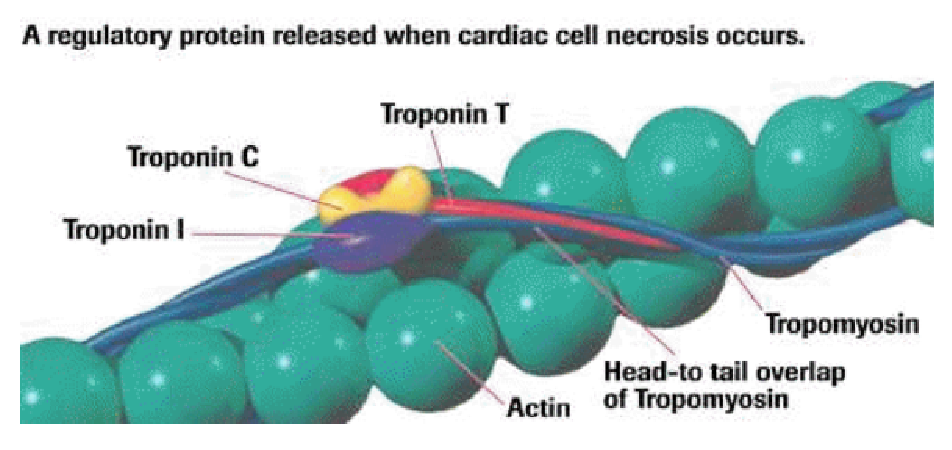
\includegraphics[height=4cm,
    angle=0]{./images/troponin.eps}}
\caption{Troponin, attached to the protein $\alpha$-tropomyosin, lies within the
groove between actin filaments.}
\label{fig:troponin}
\end{figure}

A single tropomyosin molecule spans 7 actin molecules, and is 'locked' down to
them by TnT and TnI. It also block the active sites on actin subunits.
When calcium bind to TnC, tropomyosin then rolls out of the way of the actin
active sites, allowing myosin to bind to actin, forming the cross-bridges as
described in the previous section.


\subsection{Calmodulin}

Check Sect.\ref{sec:calmodulin}

\subsection{ATP}
%\label{sec:ATP-molecule}

ATP is a mobile, rapidly-reacting $\Ca$ buffer (Sect.\ref{sec:ATP-molecule}). 


\subsection{Calbindin}
\label{sec:calbindin}

{\bf Calbindin} is a calcium-binding protein (Sect.\ref{sec:calcium-binding-proteins})
and is thus involved in calcium ion transport within cells. There are 2 types:
Calbindin 9kDa; and Calbindin 28kDa.
\begin{enumerate}
  \item reduced cytosolic $\Ca$ gradient (act as a buffer), 
  
  \item increased $\Ca$ entry into the cell (by reducing $\Ca$ near the plasma
membrane thus removing negative-feedback inhibition of $\Ca$ entry due to
$\Ca$-inactivation of ion channel), 

  \item increasing cytosolic $\Ca$ flow.
\end{enumerate}

Calbindin D-28k occurs in all major pathways of the limbic system with the
exception of the fornix (Sect.\ref{sec:Fornix}). Most of the cells containing
calbindin D-28k are vulnerable to neurodegenerative processes, e.g. in Parkinson
disease (Sect.\ref{sec:Parkinson-disease}).

Calbindin-D28k is a vitamin D responsive gene in many tissues, yet in the brain,
its synthesis is independent of vitamin D.

Calbidin-D28k has 6 EF-hands but only 4 (EF1, EF3, EF4, EF5) can function as
$\Ca$ binding sites. 

Neurons that express calbindin: Sect.\ref{sec:CB-positive-interneuron} discusses
calbindin-expressing neurons.


\subsection{Parvalbumin}
\label{sec:parvalbumin}

Parvalbumin is a calcium-binding albumin protein with low molecular weight
(typically 9-11 kDa), with 3 EF hand motifs and is structurally related to
calmodulin and troponin C. It is involved in calcium signaling. Typically, this
protein is broken into three domains, domains AB, CD and EF, each individually
containing a helix-loop-helix motif.

Other calcium-binding protein markers are calretinin (most abundant subtype in
dLPFC - Sect.\ref{sec:dLPFC}, about 50\%) and calbindin
(Sect.\ref{sec:calbindin}). Parvalbumin is a less mobile, more slowly-reacting
$\Ca$ buffer.

By using parvalbumin antibodies, parvalbumi is found in different cell types,
and they are collectively called PV-positive cells 
\begin{enumerate}
  
  \item In muscle, it is found localised in fast-contracting muscles.
  \item 
  \item  (Sect.\ref{sec:parvalbumin-positive-interneuron})
\end{enumerate}



In the rat CNS, by using parvalbumin antibodies, parvalbumin is found in many
neurons \citep{celio1990}, in particular interneurons
(Sect.\ref{sec:interneurons}).


\begin{itemize}
  \item  rich in cranial nerve nuclei related to eye movements.

  \item in a few ependymal cells and in some pillar cells of the organ of Corti

  \item  
  \item  in cells with thick, myelinated axons and restricted, focused
  projection field, i.e. different from that of calbindin
  (Sect.\ref{sec:calbindin})
  
  \item [mainly] short-axon neuron (Golgi type II): intrinsic parvalbuminic
  neurons are prominent in the cerebral cortex, hippocampus, cerebellar cortex
  and spinal cord.
  
  

  \item [smaller amount] long-axon cells (Golgi type I): Purkinje cells, neurons
  of the thalamic reticular nucleus, globus pallidus, substantia nigra (pars
  reticulata) - Sect.\ref{sec:Golgi-I-neurons}.

  \item [smaller amount] a subpopulation among large spinal-, retinal-,  
  cochlear- and vestibular ganglion cells. 
  
% Many parvalbumin-immunoreactive cells in the central nervous system are
% interneurons 
\end{itemize}



\subsection{calretinin}
\label{sec:calretinin}

Calretinin is a calcium-binding protein, serving as calcium buffers
(Sect.\ref{sec:buffers-calcium}).


Calretinin-expressing interneurons is the most abundant subtype in dLPFC -
Sect.\ref{sec:dLPFC}, about 50\%.


\subsection{SERCA pump}
\label{sec:Ca-buffer_SERCA}

SERCA pump is an ATP-driven pump, presenting at a high density in the
network SR. However, it also serves as $\Ca$ buffer as $\Ca$ bind to
its.  The amount of calcium bound on the cytosolic side may not always be equal
to the amount released on the ER side \citep{Higgins2006}. 

\subsection{Calsequestrin (CASQ)}
\label{sec:calsequestrin}

Calsequestrin (CASQ2) is a highly-capacity $\Ca$ binding protein found in SR
\citep{beard2004}. Calsequestrin (CASQ) thus has low-affinity endogenous $\Ca$
binding proteins, with $K_d\approx 0.6$mM. 

The missensed mutation CASQ2$^{D307H}$ in the highly consered region may give
rises to CPVT \citep{Lahat2001} (Sect.\ref{sec:cpvt}). However, it's unclear how
the mutation change the binding affinity of CASQ2 to $\Ca$. The study in rat
shown a reduce 60\% in $\Ca$-binding, causing a smaller $\Ca$ transient. 
\citep{houle2004} also shown that the mutation also change its interaction with RyR
linking protein, junctin and triadin. However, a recent study shown that the
mutated gene can also express and is quite stable \citep{kalyanasundaram2010}.
So, they concluded the mutation may compromise its ability to dynamically
regulate $\Ca$ buffering. 

Rapid equilibrium assumption is widely used to model buffering of calcium in the
junctional SR (jSR) \citep{greenstein2002}.
\begin{equation}
\beta_\jSR = \left( 1 +
\frac{[\B_\CSQN]K_{m,\CSQN}}{\left(K_{m,\CSQN}+[\Ca]_\ds\right)^2} \right)^{-1}
\end{equation}

\section{SR $\Ca$ content}

The SR $\Ca$ content is an important determinant for intracellular $\Ca$
transient. However, direct measurement of SR $\Ca$ content is difficult under
relatively physiological conditions, i.e. intact cardiac myocytes or isolated
myocytes \citep{bers1991ecc}. A common protocol is using caffeine to induce
releasing of $\Ca$ from SR \citep{Bassani1993}. To inhibit SERCA uptake,
thapsigargin (TG), a sesquiterpene lactone extracted from the {\it Thapsia
garganica} has been used. The graded release of $\Ca$ from SR at different
amount of $\Ca$ influx.


Thus the SR total $\Ca$ content is not consistent and
varies from 87 to 900 $\muM$ (i.e. $\mu$mol/(L cyt.)) under various condition
\citep{shannon1997} estimated intra SR free $\Ca$ to be 415$\muM$ for
cytosolic $[\Ca]_c = 100$ nM. It's expected that most of the $\Ca$ bound to low-affinity high-capacitiy $\Ca$
buffers such as calsequestrin (CSQ) (Sect.\ref{sec:RyR_CSQ_Triadin_Junctin}).

\citep{shannon1997} then performed a new measurement using Furaptra, as $K_d$ is
among the highest of the $\Ca$-dependent fluorescent dyes, i.e. measuring $\Ca$
upto 1mM. The free $[\Ca]_\sr$ as a function of cytosolic $[\Ca]_c$ is given in
Fig.\ref{fig:SR_free_Ca}.   The result showed that free SR $\Ca$ content is
700-1050 $\muM$ (i.e. $\mu$mol/(L cyt.)) for cellular value of resting $[\Ca]_c
= 100-150$ nM. The steady-state gradient between SR $\Ca$ and cytosolic $\Ca$ is
7000 based on fluorescence measurement.

\begin{figure}[hbt]
  \centerline{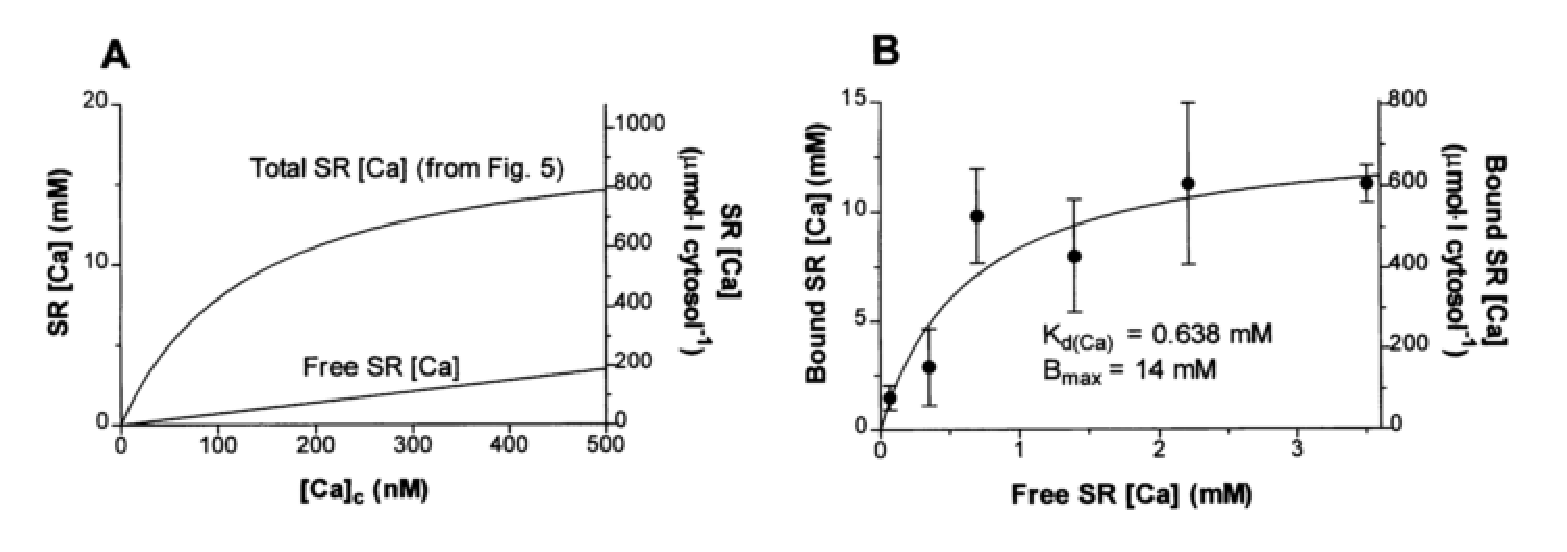
\includegraphics[height=5cm]{./images/SR_calcium_Shannon97.eps}}
\caption{SR $\Ca$ buffering curve \citep{shannon1997}}
\label{fig:SR_free_Ca}
\end{figure}

\citep{shannon1997} showed maximum SR capacity is 19 mM. The amount of
$\Ca$ binding to buffer, i.e. $[\Ca]_{\sr-b}=[\Ca]_{\sr,tot}-[\Ca]_\sr$. It's
suggested that the amount of steady-state SR total $\Ca$ content
($[\Ca]_{\sr-tot}$) is one-half of SR buffering capacity at rest, i.e. 
\begin{enumerate}
  \item method 1: $B_\max = 740 \muM$ (i.e. $\mu$mol/(L cyt.)) for a resting
  $[\Ca]_c=100$nM, and total bound $\Ca$ is 375$\muM$.
  \item method 2:$B_\max = 14$mM, with $K_d=638\muM$
\end{enumerate} 



\section{Calcium diffusion}
\label{sec:calcium_diffusion}

Another important factor contributing to the local control of calcium signalling
is the diffusion of calcium. \citep{parker1996csi} shown that diffusion within
cardiac myocytes is anisotropic though the value they derived from $\Ca$-bound
fluorescence is low. Calcium diffusion is slow in cytosol due to poorly mobile
buffers that bind to calcium \citep{hodgkin1957}. An apparent diffusion
coefficient $<r^2>$ (the mean squared displacement of the total population of
$\Ca$ ions) is defined in analogy to the conventional diffusion constant:
$D_\app=\frac{<r^2>}{6t}$. This is applied for $\Ca$ ions entering the cytosol
through an ion channel \citep{wang1993lpf}.

The diffusion coefficient of calcium in aqueous solution of
physiological ionic strength (e.g. water) is D=700-780$\mum^2$/sec
\citep{wang1953}. Due to the viscosity of cytoplasm (obstacles force diffusion
to follow convoluted force), the diffusion constant in cytosol is reduced by a
factor of 2-2.5 or $\sim 14\mum^2/$sec \citep{kushmeric1969}. In the dyadic
subspace, this will be further reduced by the presence of the 'feet' structure
\citep{sommer1976}.
\citep{soeller1997} thus estimated $D_\ca = 140\mum^2/$sec in the radial
direction and $D_\ca = 350\mum^2/$sec in the z-direction. \citep{langer1996}
used $D_\ca = 100\mum^2/$sec. \citep{pratusevich1996} used $D_\ca =
600\mum^2$/sec. \citep{smith1998, sun2000mlc,groff2008} used $D_\ca=
250\mum^2/$sec. 

Based on the comparing of wave propagation speed in the transverse and
longitudinal direction, \ce{Ca^2+} has more difficulty diffusing in transverse
than in longitudinal direction~\citep{engel1994apc}. In such cases, the
diffusion constants used were:
300$\mum^2/s$ in longitudinal and 150$\mum^2/s$ in transversal
\citep{izu2006irr}.

When modelling the transfer rate of calcium from one compartment to another,
e.g. from the subspace to the cytoplasm or from the NSR to the JSR, the
characteristic time for diffusion between compartments of two adjacent
compartments can be roughly estimated to be on the order of 
\begin{equation}
\tau \approx \frac{l^2}{D}
\end{equation}
with $l$ is the distance and $D$ is the diffusion constant. 

\subsection{Effective diffusion constants for $\Ca$}
\label{sec:effect-diff-const}



During diastole, only a very tiny fraction of $\Ca$ are
unbound~\citep{Swietach2010}, i.e.
\begin{enumerate}
\item in the cytoplasm: one in a thousand $\Ca$ ions remains unbound.
\item in the SR: one in ten remains unbound.
\end{enumerate}
Most the buffers are considerably larger than $\Ca$ ions, effective
$\Ca$ mobility is predicted to be slow. 

\begin{framed}
  \textcolor{red}{The diffusion coefficient of free Ca in the
    cytoplasm $D_{\ce{Ca}}$ is from 225-300 $\mu m^2.s^{-1}$}.
  The diffusion coefficient of mobile buffers, with molecular masses
  in the range 7-20kDa, is a factor of 2-10 smaller than that of
  $\Ca$. For small exogenous buffers like BAPTA or Fura-2, the
  diffusion coefficient may be smaller than that.
\end{framed}


\subsection{Calcium-bound Fluorescence}

For calcium-bound indicator, the diffusion is typically assume to be the same as
diffusion of free indicator. \citep{groff2008} used $D_\CaF = 32\mum^2/$sec.

\subsection{Calcium in the SR}

The fall in SR calcium during the contraction is known as $\Ca$ scraps. Within a
sarcomere, the time course of the scrap appears uniform throughout the SR,
suggesting high mobility of $\Ca$ inside the SR minimize the local calcium
gradient within.
Based from that, \citep{shannon2003cs} suggested high SR $\Ca$ mobility which is
4-5 fold higher (60$\mum^2/$sec) than calcium mobility in the cytoplasm, which
was measured to be 14$\mum^2/$sec \citep{kushmeric1969}. Other studies suggested
the similar high calcium mobility \citep{keller2007}. However, this concept was
challenged by the discovery of local depletion in JSR, known as $\Ca$ blinks
\citep{brochet2005,Kubalova2005,niggli2007}. $\Ca$ blinks occur with no apparent
change in adjacent NSR and recover to control level in 100-200ms. This
suggest the diffusion from NSR to JSR is rate limited by low mibility and high
$\Ca$ buffering in the JSR. 

\citep{swietach2008} suggested low $\Ca$ mobility in the SR by introducing a
novel method to measure $D_{\Ca,\sr}$. Caffeine microperfusion at one end of the
guinea pig or rat ventricular empties the whole SR at a rate indicating the
speed of $D_{\Ca,\sr}=8-9\mum^2$/sec. On the other hand, Bers group
estimated a higher value, about 7-fold higher \citep{wu2006}. 

\subsection{Calcium diffusion within microdomains}


In microdomain near the neighborhood of $\Ca$ channels, $\Ca$ build up within
tens of microseconds to very high value (around 100$\mu$M) and decay (within
microseconds) when channel closes. As the size and extent of this domain is
highly influenced by the presence of mobile $\Ca$ buffer, it's important to
include buffers in these studies \citep{roberts1994}. In many simplified
approximation, the stationary buffers are neglected as it's assume immobile
buffers have no influence on the steady-state distribution of free $\Ca$ and
mobile buffers.
 
When considering the diffusion of $\Ca$ from a point source (channels)
surrounded by high concentration of mobile buffers, it's reasonable to assume
the concentration of free buffers doesn't change much in the vicinity of the
channel, i.e. $\Ca$-bounded buffers move away from the vicinity and is quickly
replaced by free buffer molecules. NOTE: free $\Ca$ can reach 100$\mu$M, while
free buffers is much higher 1mM, i.e. there is maximum 10\% change with 1:1
binding ratio.

So, at short distance, the increase in free $\Ca$ above the basal level reach
the steady-state within microseconds, and is described by the equation
\begin{equation}
\Delta [\Ca] = \frac{i_\ca}{4\pi F D_\ca r} \exp(\frac{-r}{\lambda})
\end{equation}
with the first factor is ``radial diffusion'' from point source (of single
channel current $i_\ca$) - the 'geometric' aspect of radial
``unbuffered" diffusion from a point source, and the second factor (the
exponential term) is the effect of buffering with a length constant $\lambda$.
$D_\ca$ is diffusion coefficient of free $\Ca$, $\lambda$ is length constant
(the mean distant that a $\Ca$ diffuse before it is captured by a free buffer
molecule or the range of a ``non-equilibrium'' domain within which $\Ca$ is not
at equilibrium with the buffer)

\begin{equation}
\lambda = \sqrt{\frac{D_\ca}{k_\on [\B]}}
\end{equation}
with $[\B]=\frac{[\B]_{tot}.K_D}{K_D+[\Ca]}$ is the concentration of free
buffer, $k_\on$ is the rate constant of $\Ca$-bindig to the buffer.

When the buffer species is mobile and there can be many of them, we use
\citep{naraghi1997} 
\begin{equation}
\label{eq:dCa}
\Delta[\Ca] = \frac{i_\ca}{4\pi F D_\ca r}\left( \frac{D_\ca}{D_\ca+\sum_i
D_{\CaB_i}K_i} + \sum_i a_i \exp(\frac{-r}{\lambda_i}) \right)
\end{equation}
with $a_i$ is the amplitude parameter (0 or $i_\ca/(2F)$). The first term refers
to the effect when $r \le \lambda_i$ (non-equilibrium zone); and the second term
refers to the region when $r \gg \lambda_i$, i.e. buffering reaction is at
equilirbium so the effect of diffusion and equilibrium $\Ca$-binding is
formulated. 

Whene there is more than one channel, i.e. region of highly density $\Ca$
channel, we use
\begin{equation}
\Delta \Ca(t) = \frac{i_\ca}{4\pi F. D_\ca} \left(
\frac{\exp(-r_0/\lambda)}{r_0} T_0(t) + \sum_{v=1}^{n}
\frac{\exp(-r_v/\lambda)}{r_v} T_v(t) \right)
\end{equation}
$T_0(t), T_v(t)$ is time-function switching between 0 and 1 during 100-200$\mu$
of $r_v$ sufficiently short (which represent close/open state of channel). When
there are many channel, we can use ensemble average, i.e. the time-dependent
open probability $P_o(t)$.
\begin{equation}
\Delta \ca(t) = \frac{i_\ca P_0(t)}{4\pi F. D_\ca} \left(
\frac{\exp(-r_0/\lambda)}{r_0}  + \sum_{v=1}^{n}
\frac{\exp(-r_v/\lambda)}{r_v} \right)
\end{equation}





\section{Calcium in the Nucleoplasm}

Nuclear calcium have shown to play an important role in regulating gene
expression. Nuclear envelope (NE) is thapsigargin-sensitive, ER-type $\Ca$
stores. Each cytoplasmic $[\Ca]$ transient (CaT) also elicit a nucleoplasmic
$[\Ca]_\nuc$ CaT \citep{genka1999, Kockskamper2008}. Resting and diastolic
$[\Ca]_\nuc$ were always higher compared to resting $[\Ca]_\myo$
\citep{tucker1990}.
Systolic $[\Ca]_\myo$ was usually higher than $[\Ca]_\nuc$, but some cells
(15\%) exhibits higher systolic $[\Ca]_\nuc$.

The mechanism of transmitting calcium from the cytoplasm to the nucleoplasm has
not fully understood, e.g. whether it's passive diffusion through nuclear pore
complexes (NPC), or through some actively mechanism \citep{gerasimenko2004}. The
evidences for these actively mechanisms includes the presence of
$\Ca$-regulating proteins on the nuclear envelope, e.g. SERCA, $\Ca$-buffering
proteins, IP3R, or the new $\Ca$-release messenger NAADP. NAADP is nicotinic
acid adenine dinucleotide phosphate, which is believed capable of releasing
$\Ca$ from nuclear envelope by triggering RyRs. IP3R can be an important
regulator in nuclear calcium, yet its contribution to nuclear calcium signalling is poorly
understood.


The increase of $[\Ca]_\nuc$ independently from $[\Ca]_\myo$ has been implicated
in the development of cardiac hypertrophy \citep{little2009} and the progression
of heart failure. Thus, it's important to understand the relationship between
$[\Ca]_\nuc$ and $[\Ca]_\myo$.

\citep{bootman2000, echevarria2003, badminton1996}.



\section{Cell preparation}

\citep{} discuss standard method. 

Following anesthesia the rat (pentobarbital, 100 mg/kg), the heart of the rat is
removed from the chest using Langendorff method. The heart is provided with
oxygen and metabolites via a single cannula inserted into the ascending aorta.
In particular, the oxygenated blood (a perfusate) is pumped down the aorta
towards the heart by means of an external pump
\footnote{\url{http://www.visibleheart.com/methods.shtml}}. 


%%% Local Variables: 
%%% mode: latex
%%% TeX-master: "mainfile"
%%% End: 
